\documentclass[mtech,copromote]{PETthesis}
\setcounter{secnumdepth}{3}
\setcounter{tocdepth}{3}
%% The options here are
%% btech, if you do your proposal for your B Tech project mini-thesis
%% mtech, if you do your proposal for your M Tech dissertation
%% dtech, if you do your proposal for your D Tech thesis
%% mtechbis, if you do the dissertation component of the M Tech (Business Administration
%% copromote, if you are being co-promoted
%% prepare, if you want to save a page initially with the title page - also datestamp the copy
\title{A Model for Recommending Related Research Papers: A Natural Language Processing Approach}
\author{Juandre Anton van Heerden}        % use your full names
\thesismonth{December}
\thesisyear{2021}
\thesispromoter{Prof. Reinhardt A. Botha}     % use abbreviations for second names
\thesiscopromoter{Prof. Bertram P. Haskins}          % Only makes a difference if copromote
                                        % option specified in class

%% I suggest that you always include these packages
\usepackage{graphicx}   % to use eps graphics
\usepackage{lscape}
\usepackage{svg}
\usepackage{amsmath}
\usepackage{apacite}    % enable apa citations to be formatted correctly
\usepackage{url}        % handle urls that need to break accross lines
\usepackage{booktabs}   % a bit nicer tables than the standard -- not part of standard distribution
\usepackage{amsthm }    % for having nice definition and theorem environments
\usepackage{amsmath}
\usepackage{titlesec}
\usepackage{verbatim}
\usepackage{listings}
\usepackage{float}
\usepackage{color,soul}
\usepackage[flushleft]{threeparttable}
\usepackage{xcolor}
\usepackage{colortbl}
\usepackage{multirow}
\usepackage{tabularx}
\usepackage{arydshln}
\usepackage{pdfpages}
\usepackage{tcolorbox}
\usepackage{dirtytalk}
\usepackage[utf8]{inputenc}
%\usepackage{todonotes}
\usepackage[normalem]{ulem}




\useunder{\uline}{\ul}{}

\definecolor{codegreen}{rgb}{0,0.6,0}
\definecolor{codegray}{rgb}{0.5,0.5,0.5}
\definecolor{codepurple}{rgb}{0.58,0,0.82}
\definecolor{backcolour}{rgb}{0.95,0.95,0.92}

\lstdefinestyle{mystyle}{
    backgroundcolor=\color{backcolour},   
    commentstyle=\color{codegreen},
    keywordstyle=\color{magenta},
    numberstyle=\tiny\color{codegray},
    stringstyle=\color{codepurple},
    basicstyle=\ttfamily\footnotesize,
    breakatwhitespace=false,         
    breaklines=true,                 
    captionpos=b,                    
    keepspaces=true,                 
    numbers=left,                    
    numbersep=5pt,                  
    showspaces=false,                
    showstringspaces=false,
    showtabs=false,                  
    tabsize=2
}
 
\lstset{style=mystyle}
\newtheorem{lesson}{Lesson}

%\graphicspath{{./eps/}} % keep those large eps files in separate sub-directory
                        % one down from current directory  -- if you want to that is

\bigspace               % enables the one-and-half spacing (about) for the document
                        % if you need to use single spacing in eg a table
                        % switch to \smallspace and immediately afterwards
                        % use \bigspace again

%\includeonly{Chapter1, Chapter8}

\begin{document}

% This next part sets up my list of caveats that I'm going to use later in the document
% It uses the package amsthm

\theoremstyle{plain}               % make a theory type called cav
\newtheorem{cav}{Caveat}           % of type plain
\theoremstyle{remark}              % and one called sol,
\newtheorem{sol}{Solution}         % of type remark
                                   % which would be numbered as "Caveat 1", "Solution 1", etc.
                                   % plain = title and number bold, rest italics
                                   % definition = title and number bold and rest normal
                                   % remark = title and number in italics and text normal
                                   % Obviously the name (cat, sol) can be anything...

%\setcounter{secnumdepth}{4}
\maketitle
%% This maketitle will generate
%% If not in prepare mode
%%   -- a coverpage (title and name)
%%   -- a title page with the relevant rhymes :-)

%------------------------------%
% Start of the actual document %
%------------------------------%

% FIRST ALL THE INTRO JUNK
% Typically that include
% -- an appropriate declaration (see the example in frontstuff.tex) mandatory for M and D's)
% -- Abstract (mandatory for all)
% -- Acknowledgements (that's where you thank me - hie-hie)
%\hyphenation{informa-tion security culture factor achieving Governance CGICT General F-CGICT}   %Words to hyphenate or NOT
\frontmatter           % Sorts out the different page numbering, heading numbering etc.
\chapter{Declaration}

I, \thethesisauthor, hereby declare that:

\begin{itemize}

\item The work in this dissertation is my own work.

\item All sources used or referred to have been documented and
recognised.

\item This \MakeLowercase{\thethesistype} has not previously been
submitted in full or partial fulfilment of the requirements for
an equivalent or higher qualification at any other recognised
educational institute.

\end{itemize}

%% You could of course include your signature electronically if you want to be fancy
%% Scanning and convert to eps should do the trick
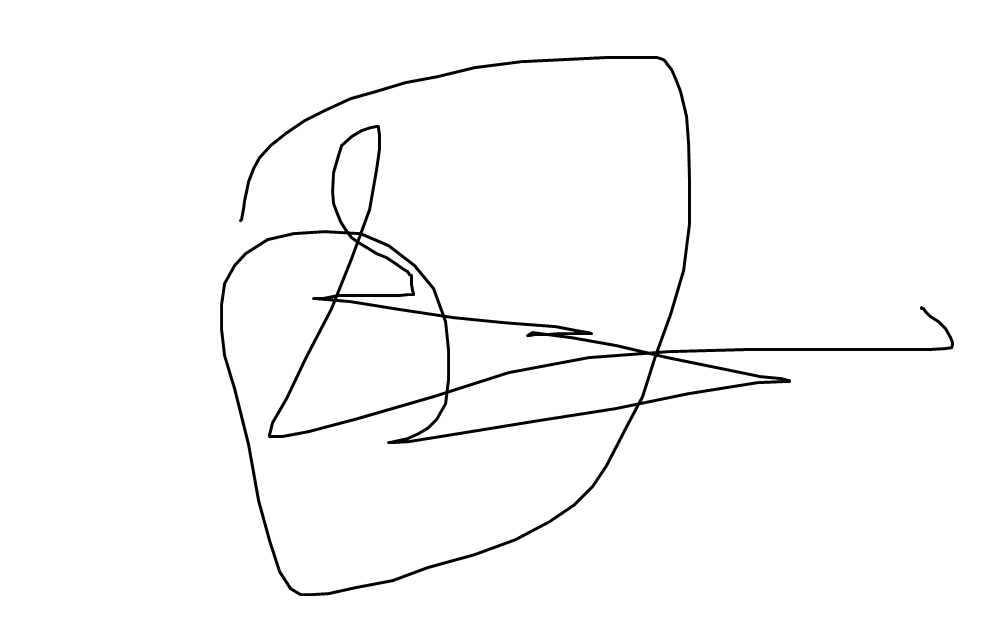
\includegraphics[width=40mm]{./figures/signature}
%% or you could just leave some space for it
\rule[0mm]{0mm}{40mm}

\rule[0mm]{70mm}{0.3mm}

\thethesisauthor

\chapter*{}
This thesis is dedicated to the memory of my father, \textbf{Anton van Heerden}.


\chapter{Acknowledgements}

Foremost, I would like to express my sincere gratitude to my supervisors Prof. Reinhardt A. Botha and Prof. Bertram P. Haskins for their continuous support during my Master's study. Furthermore, I would like to express my gratitude for their patience, motivation, enthusiasm, and immense knowledge. Their guidance assisted me throughout the research and writing of this dissertation. I could not have imagined having better supervisors for my Master's study.

Furthermore, I would like to thank the following benefactors for their financial assistance:

\begin{itemize}
	\item The financial assistance of the National Research Foundation (NRF) towards this research is hereby acknowledged. Opinions expressed and conclusions arrived at, are those of the authors, and are not necessarily to be attributed to the National Research Foundation.
	\item The financial assistance of the Nelson Mandela University's Post Graduate Research Scholarship (PGRS) is also hereby acknowledged.
\end{itemize}

Finally, I must express my very profound gratitude to my family for providing me with unfailing support and continuous encouragement throughout the process of researching and writing this dissertation. This accomplishment would not have been possible without you. Thank you.

\chapter{Abstract}
The volume of information generated lately has led to information overload, which has impacted researchers’ decision-making capabilities. Researchers have access to a variety of digital libraries to retrieve information. Digital libraries often offer access to a number of journal articles and books. Although digital libraries have search mechanisms it still takes much time to find related research papers.

The main aim of this study was to develop a model that uses machine learning techniques to recommend related research papers. The conceptual model was informed by literature on recommender systems in other domains. Furthermore, a literature survey on machine learning techniques helped to identify candidate techniques that could be used.

The model comprises four phases. These phases are completed twice, the first time for learning from the data and the second time when a recommendation is sought. The four phases are: (1) identify and remove stopwords, (2) stemming the data, (3) identify the topics for the model, and (4) measuring similarity between documents.

The model is implemented and demonstrated using a prototype to recommend research papers using a natural language processing approach. The prototype underwent three iterations. The first iteration focused on understanding the problem domain by exploring how recommender systems and related techniques work. The second iteration focused on pre-processing techniques, topic modeling and similarity measures of two probability distributions. The third iteration focused on refining the prototype, and documenting the lessons learned throughout the process. Practical lessons were learned while finalising the model and constructing the prototype. These practical lessons should help to identify opportunities for future research.
   % This file contains examples of the above
                       % Off course then there is the customary table of contents etc.
\tableofcontents

\listoftables

\listoffigures

\lstlistoflistings

\mainmatter            % Sorts out the different page numbering, heading numbering etc.

%% At the M and D level your dissertation/thesis are often consisting of
%% distinct parts, each containing several chapters
%% Typical Parts = Introdustion, Model development, Epiloque/Evaluation
%% These can be indicated with \part commands

%\part{Dissertation}

%% Each chapter can now be included
%\chapter{Declaration}

I, \thethesisauthor, hereby declare that:

\begin{itemize}

\item The work in this dissertation is my own work.

\item All sources used or referred to have been documented and
recognised.

\item This \MakeLowercase{\thethesistype} has not previously been
submitted in full or partial fulfilment of the requirements for
an equivalent or higher qualification at any other recognised
educational institute.

\end{itemize}

%% You could of course include your signature electronically if you want to be fancy
%% Scanning and convert to eps should do the trick
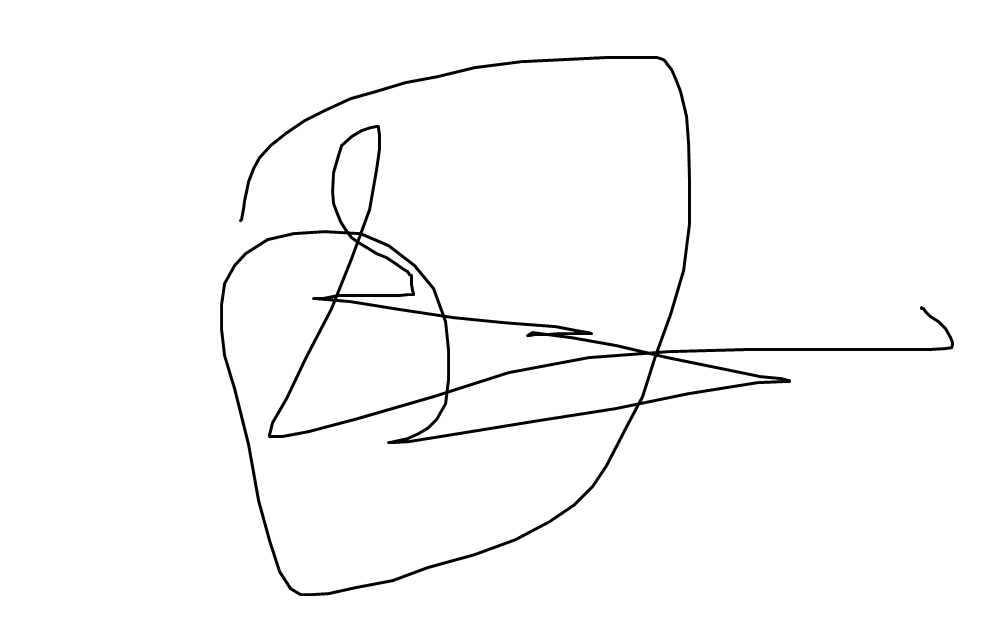
\includegraphics[width=40mm]{./figures/signature}
%% or you could just leave some space for it
\rule[0mm]{0mm}{40mm}

\rule[0mm]{70mm}{0.3mm}

\thethesisauthor

\chapter*{}
This thesis is dedicated to the memory of my father, \textbf{Anton van Heerden}.


\chapter{Acknowledgements}

Foremost, I would like to express my sincere gratitude to my supervisors Prof. Reinhardt A. Botha and Prof. Bertram P. Haskins for their continuous support during my Master's study. Furthermore, I would like to express my gratitude for their patience, motivation, enthusiasm, and immense knowledge. Their guidance assisted me throughout the research and writing of this dissertation. I could not have imagined having better supervisors for my Master's study.

Furthermore, I would like to thank the following benefactors for their financial assistance:

\begin{itemize}
	\item The financial assistance of the National Research Foundation (NRF) towards this research is hereby acknowledged. Opinions expressed and conclusions arrived at, are those of the authors, and are not necessarily to be attributed to the National Research Foundation.
	\item The financial assistance of the Nelson Mandela University's Post Graduate Research Scholarship (PGRS) is also hereby acknowledged.
\end{itemize}

Finally, I must express my very profound gratitude to my family for providing me with unfailing support and continuous encouragement throughout the process of researching and writing this dissertation. This accomplishment would not have been possible without you. Thank you.

\chapter{Abstract}
The volume of information generated lately has led to information overload, which has impacted researchers’ decision-making capabilities. Researchers have access to a variety of digital libraries to retrieve information. Digital libraries often offer access to a number of journal articles and books. Although digital libraries have search mechanisms it still takes much time to find related research papers.

The main aim of this study was to develop a model that uses machine learning techniques to recommend related research papers. The conceptual model was informed by literature on recommender systems in other domains. Furthermore, a literature survey on machine learning techniques helped to identify candidate techniques that could be used.

The model comprises four phases. These phases are completed twice, the first time for learning from the data and the second time when a recommendation is sought. The four phases are: (1) identify and remove stopwords, (2) stemming the data, (3) identify the topics for the model, and (4) measuring similarity between documents.

The model is implemented and demonstrated using a prototype to recommend research papers using a natural language processing approach. The prototype underwent three iterations. The first iteration focused on understanding the problem domain by exploring how recommender systems and related techniques work. The second iteration focused on pre-processing techniques, topic modeling and similarity measures of two probability distributions. The third iteration focused on refining the prototype, and documenting the lessons learned throughout the process. Practical lessons were learned while finalising the model and constructing the prototype. These practical lessons should help to identify opportunities for future research.

%\part{Introduction}
\chapter{Introduction}
\label{chap: Chapter 1}

Academic content generation has seen an increase in recent years. Getting usable research papers has become a problem. In order to produce reputable and quality papers, vast amounts of research need to be consulted in several domains and sub-domains. Reading and working through the additional research papers can be time consuming and could result in researchers overlooking important topics and discussions.

This study is a exploratory study into how machine learning (ML) coupled with natural language processing can aid in identifying usable research papers with less effort. However, it quickly became clear that machine learning and natural language processing is rich in aiding techniques and algorithms.

This chapter sets the groundwork of the research project. The problem area consists of a brief introduction into machine learning, topic modeling and clustering techniques, leading to the problem statement. In addition, research objectives are identified. Thereafter, the research process is described which was followed to achieve the research objectives. The chapter ends with the chapter outline for the rest of the dissertation and a brief conclusion to the chapter.


\section{Background}

Information overload is a real phenomenon in our digital age, and our access to knowledge and resources have exceeded our capacity to comprehend. The emergence of online databases has made the ability to search, find, retrieve and summarise documents increasingly difficult. The possibilities have increased drastically in recent years of using machine learning (ML), information retrieval (IR) and natural language processing (NLP) to ease this immense task of navigating through the same databases.

\citeA{Andriybook2019} describes machine learning as a subfield of computer science, which uses algorithms to help identify certain objectives. There are three paradigms of machine learning:

\begin{enumerate}
    \item Reinforcement learning – primarily focuses on training machine learning models to perform a sequence of decisions based on data \cite{DBLP:journals/corr/abs-1806-08894}.
    \item Supervised learning – is a machine learning task that maps input to output based on tagged or labelled datasets \cite{singh2019natural}.
    \item Unsupervised learning – is defined as mapping inputs to outputs but the datasets do not contain any tagging or labels \cite{hastie2009unsupervised}.
\end{enumerate}

Information retrieval is a mixture of information systems, databases and data mining techniques \cite{baeza1999modern}. Furthermore, \citeA{baeza1999modern} mentioned that information retrieval includes techniques which aid searching for information in a document. Another technique, called text mining, also intersects information retrieval and machine learning.

The text mining approach seeks to identify words and phrases that could explain certain underlying structure in the data. Text mining has focused on analysing co-occurrence data through association rules, distribution analysis, and different clustering approaches. Utilising these approaches to create practical categories rather than using predefined categories, opens up a world of new research options. \citeA{hofmann2017probabilistic} suggests that topic modeling would be a useful tool to extract information from textual data.

\section{Description of Problem Area} \label{ssec:prob}

As mentioned in the previous section, information overload has become a real problem in recent years. More specifically, researchers have indicated that information overload has caused three main difficulties \cite{al2021exploring}. They are; difficulty to process the information which was collected, difficulty to find relevant and quality information and lastly, there are just too much information generated.

Researchers experience difficulty when seeking information they develop cognitive barriers \cite{savolainen2015cognitive}. Five sub-types of cognitive barriers are reported by the study: (1) not able to differentiate between the information needs and the research needs, (2) inability to formulate information needs, (3) not aware of the various information sources, (4) low self-efficacy, and (5) unable to deal with information overload.

The best way to combat information overload from an personal and technological perspective, is better designed information systems. Such information systems will enable the researcher to better balance the scale between consuming information and understanding it \cite{bawden2020information}.



As mentioned in the previous section, information overload has become a real problem in recent years. More specifically, researchers have indicated that information overload has caused three main difficulties \cite{al2021exploring}. They are: difficulty to process the information which was collected; difficulty to find relevant and quality information; and lastly, there is just too much information generated.

Researchers experiencing difficulty when seeking information develop cognitive barriers \cite{savolainen2015cognitive}. Five sub-types of cognitive barriers are reported by the study: (1) not being able to differentiate between information needs and research needs, (2) inability to formulate information needs, (3) not being aware of the various information sources, (4) low self-efficacy, and (5) inability to deal with information overload.

The best way to combat information overload from both a personal and a technological perspective, is to have better designed information systems. Such information systems will enable the researcher to balance the scale better between consuming information and understanding it \cite{bawden2020information}.

This leads to the following problem statement:

\textbf{\textit{To identify related research papers is a time consuming cognitive barrier.}}

\section{Research Objective} \label{ssec: Chapter 1}

Research objectives are derived from the problem statement. In order to satisfy the problem described above, the primarily research objective is to:

\textbf{\textit{Develop a model to recommend related research papers}}

This model is to be developed with the intention of aiding academics in any research field. For this to be achieved, the following sub-objectives must be achieved:
\begin{itemize}
  \item[SO1:] To identify recommender systems techniques and how they are used.
  \item[SO2:] To identify machine learning techniques that assist with the recommender task.
\end{itemize}

The model will include recommender system- and machine learning techniques. The development of the prototype is to show that the model is feasible to implement. Furthermore, it serves to demonstrate applicability by using information security South Africa data. Throughout the development of the model and prototype practical lessons were learned, which will be discussed in Chapter \ref{chap: Chapter 7}.

In the next section, the research process will be discussed.

\section{Research process}

Owing to the fact that this research study is primarily experimental in nature, a model and a prototype were developed. A broader explanation of the paradigm, the research position itself, and also which methods were used throughout the study, are presented in Chapter \ref{chap: Chapter 4}.

\section{Delineation}

This study included the development of a prototype that was built using text mining and natural processing techniques. Furthermore, the techniques used were not chosen based on experimentation but were derived from literature. 
The prototype was developed to only identify topics and needs a certain level of manual intervention to validate the recommendations.
The prototype was done in the Python 3 environment and used several NTLK and Gensim libraries. The dataset was obtained and used which was made available on the Information Security South Africa website. 


\section{Ethical Consideration}

No ethical clearance was needed to complete this study. All of the data was used from a publicly available source and do not contain personal or sensitive data. No human interaction was needed to complete this study.

\section{Chapter Outline}
Figure \ref{fig:Dlayout} provides the layout of this dissertation. It can be categorised into three parts: 
\textit{Introduction, prototype development, and lessons learned and conclusion.}

The \textit{Introduction} part includes Chapter \ref{chap: Chapter 1} to \ref{chap: Chapter 3}.
Chapter \ref{chap: Chapter 1} provides the introduction and background to this study. This is followed by the problem statement and the objectives. Lastly, it refers to the research process, which will be discussed in Chapter \ref{chap: Chapter 4}. Chapter \ref{chap: Chapter 2} focuses on recommender systems and what constitutes a recommendation task. Furthermore, it discusses each recommender system method, along with examples of each. Chapter \ref{chap: Chapter 3} investigates the various machine learning technologies that were considered in this study. Chapter \ref{chap: Chapter 3} concludes by investigating document clustering and which techniques should be used.

The \textit{model development} part includes Chapters \ref{chap: Chapter 4} to \ref{chap: Chapter 6}. Chapter \ref{chap: Chapter 4} focuses on the research process which was followed in this study, highlighting the research methods used. Chapter \ref{chap: Chapter 5} deals with the development of the model derived from the research design chapter. Chapter \ref{chap: Chapter 6} outlines the techniques and methods that were used in the development. 

As seen in Figure \ref{fig:Dlayout}, Chapter \ref{chap: Chapter 6} is created with a dual purpose: (1) while developing the prototype, certain parameters were identified which influenced the quality of the prototype and model, (2) using recommender system concepts, machine learning algorithms and data from an information security conference showed that the model was applicable and feasible.

The \textit{lessons learned and conclusion} part includes Chapter \ref{chap: Chapter 7} and Chapter \ref{chap: Chapter 8}. 
Chapter \ref{chap: Chapter 7} focuses on practical lessons learned during the development of the model and prototype. Chapter \ref{chap: Chapter 8} concludes the study by summarising it and revisits the research objectives and hints to further research to be done.


The \textit{lessons learned and conclusion} part includes Chapter \ref{chap: Chapter 7} and Chapter \ref{chap: Chapter 8}. Chapter \ref{chap: Chapter 8} focuses on practical lessons learned during the development of the model and prototype. Chapter \ref{chap: Chapter 8} concludes the study by summarising it. It revisits the research objectives and hints at further research to be done.

\begin{figure}[htbp]
\centering
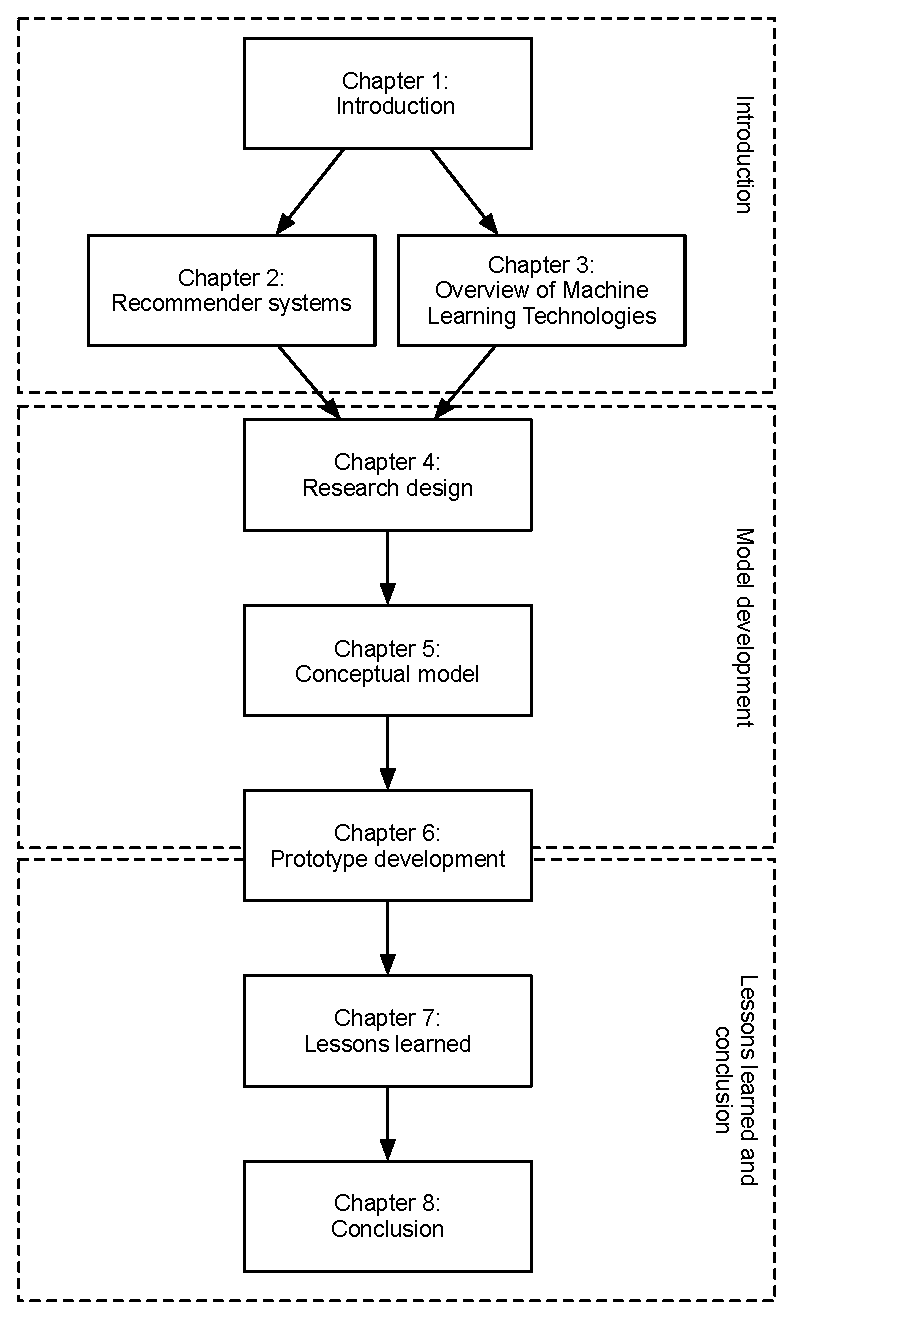
\includegraphics[width=10cm]{./figures/overlast222.eps}
\caption{Layout of the Dissertation}
\label{fig:Dlayout}
\end{figure}

%\part{Background}
\chapter{Recommender Systems}
\label{chap: Chapter 2}

The focus of this chapter is to identify a research problem and methodology which needs to be followed.

In this chapter, we discuss the background and related work of recommender systems. The following section discusses the history of information retrieval and how it ties in with information filtering. After that, the various methods of recommender systems will be addressed. In the latter sections, a high-level overview will be discussed of the components in a recommender system. The chapter concludes with state-of-the art recommender systems.

\section{Information Retrieval}

We live in an information age surrounded by technology. Information is the lifeblood of the technological ecosystem that is spread using smartphones, tablets, and other computing devices. Owing to technological advances, information is easily created or distributed. It is apparent that with the ever-increasing creation of information, researchers are experiencing information overload, which has a direct influence on academic performance \cite{binti2017influence}.

Information overload can be defined as when an individual, who needs to make a decision, is trying to ingest a large amount of data, and the amount of data is larger than the individual’s capacity to process the information \cite{Heylighen2002ComplexityAI}.
Researchers have learned to combat information overload by employing tools consisting of new technology to expose only the information that is relevant to them, known as information filtering \cite{Hanani2001}. 

Information filtering systems stretch across multiple domains and are useful for extracting information out of unstructured or semi-structured information bodies like e-mails and documents, for large amounts of text, and lastly, it can also keep account of  the activities of various user profiles.

The above features are not only limited to information filtering systems but also information retrieval. It is important to remember that information filtering and information retrieval do work similarly, but differ in characteristics indicated below, and in summary in Table \ref{tab:DIFCBFIR}.

\begin{enumerate}
    \item Frequency of use – information retrieval [IR] systems are designed for one-time, ad hoc users, whereas information filtering [IF] systems are created for repetitive uses.
    \item Representation of information needs – in information retrieval systems, users interact with queries. In contrast, in information filtering systems, the long-term needs of users are best saved in user profiles.
    \item Goal – information retrieval systems select the information stated in the query out of the database. Information filtering systems just filter out irrelevant data.
    \item Database – information retrieval systems usually employ static databases to store and retrieve information. Information filtering works with dynamic data.
    \item Types of users – information retrieval systems do not know the users, and anyone can pose a query. Users of information filtering systems need to be known, since the system has models of all the user profiles.
    \item Index – information retrieval systems index data based on items and information filtering systems index based on user profiles.
\end{enumerate}

\begin{table}[]
\centering
\resizebox{\textwidth}{!}{%
\begin{tabular}{|l|l|l|}
\hline
\textbf{Characteristics}     & \textbf{Information Retrieval}                                                                                                    & \textbf{Information Filtering}                                                                                                                                   \\ \hline
Frequency of use             & ad-hoc use                                                                     & \begin{tabular}[c]{@{}l@{}}long term users \end{tabular}                                                     \\ \hline
Representation of information needs & queries                                                                                                        & user profiles                                                                                                                                  \\ \hline
Goal                         & \begin{tabular}[c]{@{}l@{}}selecting relevant items \end{tabular} & \begin{tabular}[c]{@{}l@{}}filtering out irrelevant data\end{tabular} \\ \hline
Database                     & static                                                                                                         & dynamic                                                                                                                                        \\ \hline
Type of users                & not known to the system                                                                                        & \begin{tabular}[c]{@{}l@{}}known to the system,\\ a user model\\ is saved in the system\end{tabular}                                           \\ \hline
Index              & items                                                                                        & \begin{tabular}[c]{@{}l@{}}user profiles\end{tabular}                                                        \\ \hline
\end{tabular}%
}
\caption{Comparison between IR and IF systems}
\label{tab:DIFCBFIR}
\end{table}

As highlighted in Table \ref{tab:DIFCBFIR}, information retrieval and information filtering does work similarly but there are some differences at their core. \citeA{resnick1997} mention that sources suggest using recommender systems to tailor content to users.

The aim of information filtering (IF) is to show only the items that are relevant to the users \cite{Hanani2001}. The idea was that Information Filtering can be more effective when humans are involved in the filtering process \cite{Hanani2001}.

Because the spike of product information makes it harder for users to find what they are looking for online, e-commerce sites like Amazon.com use collaborative filtering based on purchase history and customer ratings to make personalised recommendations.

Since the introduction of collaborative filtering in the 1990s, recommender systems have grown to be a very important research area \cite{resnick1994grouplens,shardanand1995social}. The term ‘collaborative filtering’ was coined in 1992 by Goldberg when implementing one of the first spam-filtering systems \cite{goldberg1992using}.

‘A recommender system is defined as a tool that can recommend a list of items to a particular set of users based on the user’s preferences’ \cite[p.~4]{ricci2011introduction}.

They have successfully applied recommender systems to different domains such as e-commerce, movies, news, music, research, just to name a few. For example, on Amazon and Netflix users buy and watch more content that is recommended to them \cite{Andre2018} now that the gravity of recommender systems is emphasised.

\citeA{adomavicius2005toward} have identified three types of recommendation methods. They are:
\begin{enumerate}
    \item Collaborative filtering (CF)
    \item Content-based filtering (CBF)
    \item A hybrid method
\end{enumerate}
In the following section, we will discuss the various types of recommendation methods.

\section{Collaborative Filtering (CF)}  \label{sec:collab}

Collaborative filtering systems assume that a user will like the same items as another user liked in the past. Collaborative filtering systems are popular and are commonly used in online shopping websites \cite{Nilashi20161}.

Collaborative filtering focuses recommendations based on similarities between user ratings. Content-based filtering works a bit differently from collaborative filtering, in that users get recommendations based on other users’ preferences in the past. Lastly, the hybrid recommender system employs both collaborative filtering and content-based filtering methods.

In recent years, researchers adapted the traditional content-based filtering approach to move towards preference-based filtering. This subdomain focused on predicting items based on the users’ preferences \cite{william1999learning,freund2003efficient,jin2002preference,jin2003collaborative}. For example, preference-based filtering can predict movies based on their order relative to each other and not on individual ratings. As stated in the delineation of this dissertation, the focus will be on rating like-based recommendations since it is a popular approach \cite{park2012literature}.

The collaborative filtering (CF) approach works by predicting user preferences for items through learning from past user-item relationships \cite{celma2008new}. Users give feedback to the system through their preferences or ratings and then the recommender system provides a list based on the feedback.

One of the first recommender systems that used the collaborative filtering method was Ringo, a music recommender system \cite{shardanand1995social}. A few other systems that have employed collaborative filtering in that time period can be found in \citeA{resnick1994grouplens}.

Each method has several advantages and disadvantages, which would guide recommender system implementation to fit the use case.
An argument in favour of using collaborative filtering is that implementing Memory based filtering is easy \cite{Girase}. For example, memory-based methods use historic rating data between users or items to recommend items to people. Another positive aspect is that memory-based filtering would be preferred when new data is continuously supplied to the model \cite{jannach2010recommender}. Full updates can be made  continuously to the recommending system.

In contrast to the advantages of collaborative filtering, it also does have disadvantages. Some occur when collaborative filtering runs into a general issue called the cold start problem. That is when a new user is introduced to the system, and the system does not know what to recommend to the user.

Collaborative filtering is also less scalable since some systems generate recommendations for billions of user-item pairs. Finally, in some cases, collaborative filtering systems have been found to be manipulated by users promoting their own items \cite{resnick1994grouplens}.

Collaborative filtering is classified into two methods: memory-based- and model-based collaborative filtering \cite{naak2009multi}.

\subsection{Model based collaborative filtering} 

This creates and builds an offline statistical model based on the user-item pairs seen in the training set. Once the model has been built, it is then applied in an online setting to recommend as intended \cite{jannach2010recommender}. Several techniques are being used in model-based collaborative filtering, such as probabilistic techniques \cite{pavlov2004collaborative}, and graph- based techniques \cite{clements2009exploiting}.

The preferred ones are the latent factor models that reduces the dimensionality of the matrix and uncover latent topics between users and items. Some examples of latent factor models include: singular value decomposition (SVD) for matrix factorisation \cite{clements2009exploiting} and probabilistic latent semantic analysis (pLSA).


\subsection{Memory based collaborative filtering}
\citeA{jannach2010recommender} describe memory-based collaborative filtering as recommendations that are being made on the entire user-item rating matrix. It computes distance or correlation measures to find user/item similarities. Furthermore, memory-based collaborative filtering looks for either neighboured users for the target user, user-based, or pairs of items that are rated by other users (item-based).

In the next section, the content-based filtering method will be discussed, followed by its advantages and disadvantages.

\section{Content-based Filtering} \label{sec:content}
The content-based approach to recommendation has its roots in the information retrieval (IR) and information filtering (IF) research field. Recently, much research has been undertaken in the recommendation systems, information retrieval and information filtering fields.

Pushing the boundries in terms of what each field can do, content-based filtering methods analyse a set of features of items that are relevant to the user and link the user profile based on those items. In essence, the method links the users to the items \cite{lops2011content}.

There are a few comparisons that can be made between content-based filtering and IR, outlining the differences and similarities \cite{belkin1992information}. The common goal between content-based filtering and IR systems is to select items that are relevant to the users.

For example, suppose the user is looking for a similar or set of similar research papers. In that case, the content-based recommender system will recommend research papers based on the themes found in the current paper; thus, leading us to the advantages and disadvantages of content-based recommender systems.

One of the disadvantages found in collaborative filtering, is a strength in content-based filtering. In contrast to collaborative filtering, the cold-start problem does not apply to content-based filtering since the recommendations are not made based on ratings from other users.

In addition to the non-existent cold-start problem, building a content-based filtering recommender system is straightforward and significant in terms of  adding incremental data to the models.

On the other hand, content-based filtering does have difficulty in generating the features of the items. There are limits to the number and types of features that one can generate from items.

In addition to the features, domain knowledge is needed. For example, for research paper recommendations, the system needs to have quite a lot of data regarding each document, including data such as what topics are being discussed, and which branch in that specific topic are being covered. The system needs to distinguish between what the user likes and what not \cite{lops2011content}.

Content-based filtering often suffers from over-specialisation since it recommends the same types of item. For example, when inputting a ransomware research paper into the recommender system, it will only show research papers which also contain ransomware-related topics. This issue is called serendipity. Content-based recommender systems tend to lack novelty awareness \cite{shah2018}.

In the next section, the high-level architecture of a recommender system will be discussed.

\section{High level Architecture of Recommender Systems}

\begin{figure}[htbp]
\centering
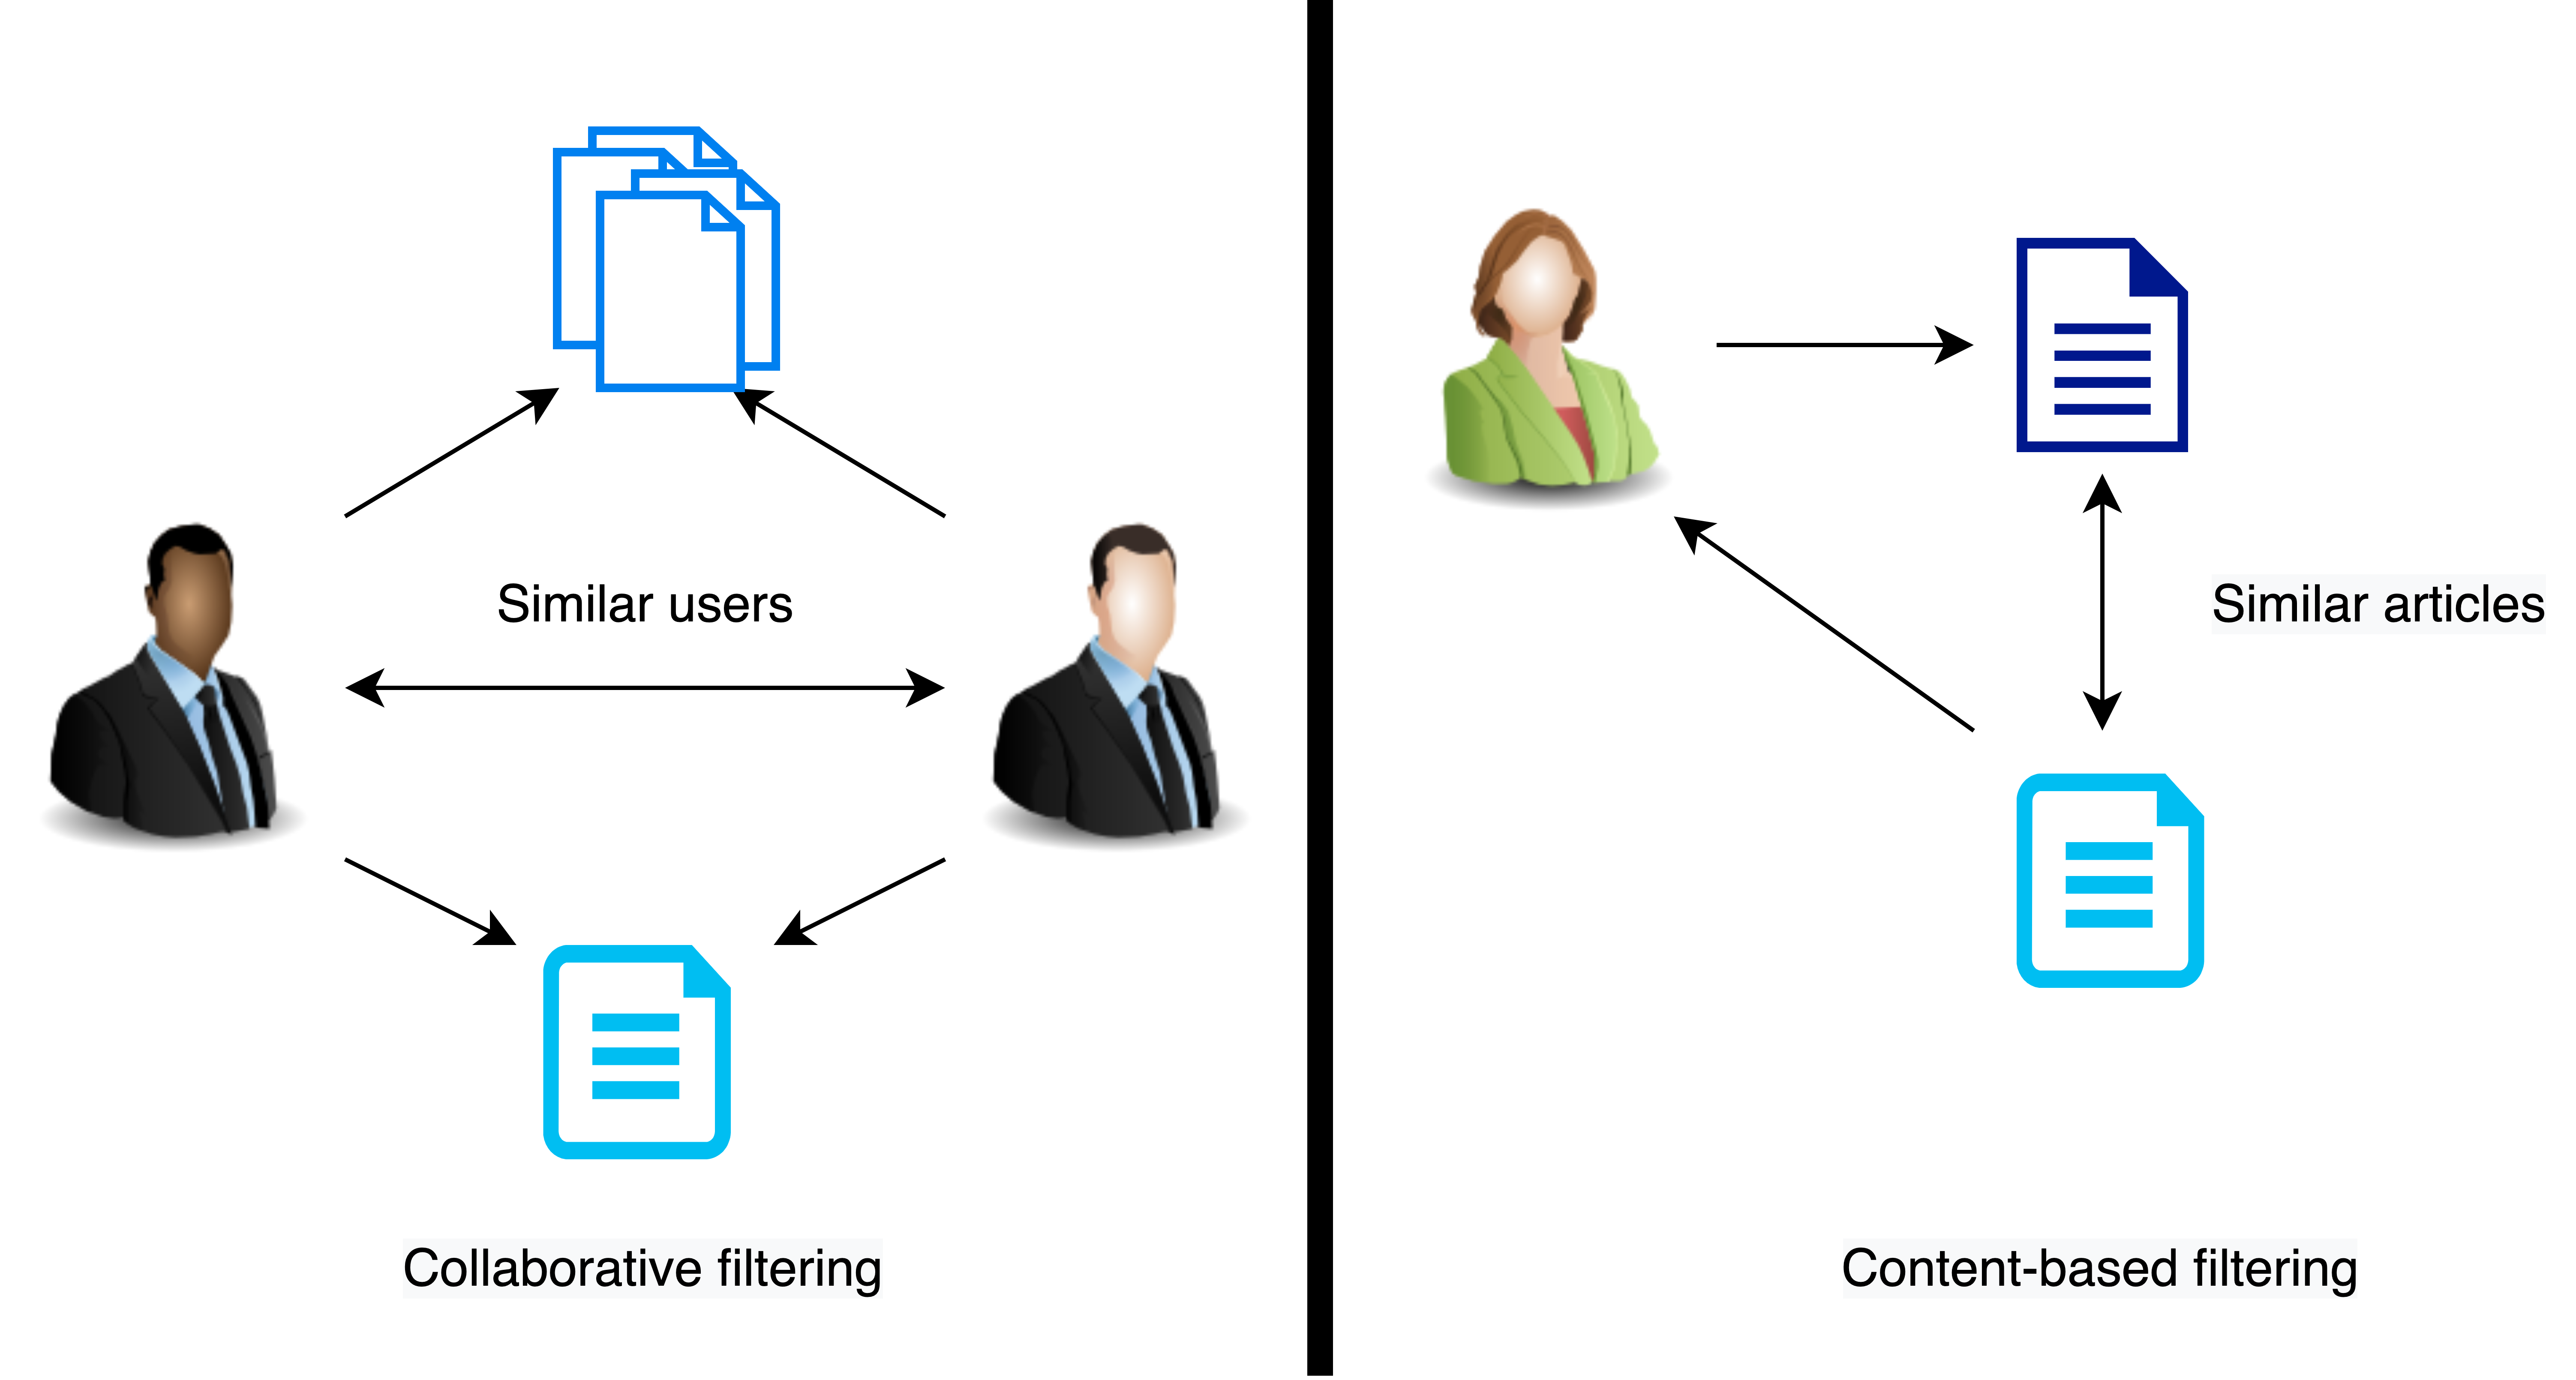
\includegraphics[width=10cm]{./figures/overviewRS1.png}
\caption{Overview of Recommender Systems}
\label{fig:OverviewRS}
\end{figure}

This section focuses on introducing the high-level architecture of a recommender system. Each component will be discussed in relation to collaborative filtering and content-based filtering methods.

As seen in Figure \ref{fig:OverviewRS}, in both recommender system methods, we see similar components. One component is that of similarity, either between articles or between other users. Both of the methods have a learning component where machine learning or information retrieval methods can be employed.

More components will be introduced later in this section. Recommender systems are strung together to attain a certain goal. The high-level architecture, portrayed in Figure \ref{fig:archRS}, will be discussed now:

\begin{figure}[htbp]
\centering
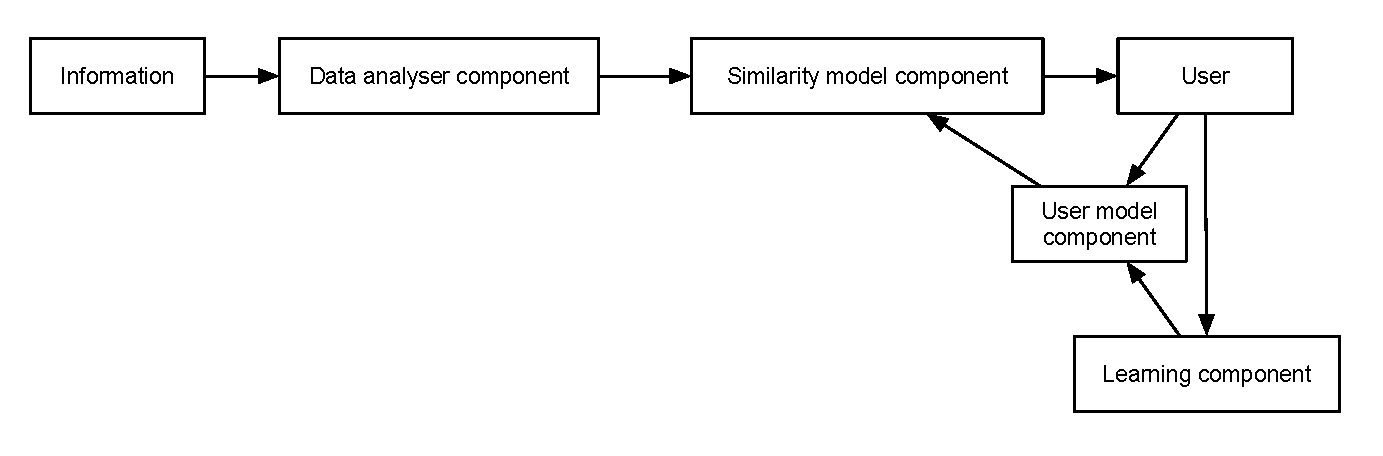
\includegraphics[width=12cm]{./figures/arch12.eps}
\caption{Architecture of Recommender Systems}
\label{fig:archRS}
\end{figure}

\begin{itemize}
    \item The data analyser component – the items are obtained or collected (e.g. documents) from information providers. The items are then analysed and represented in a readable format (e.g. in a vector of index terms).
    Such a vector will be the input to the similarity model component.
    \item The user/item model component – it gathers information about the user and their needs (explicitly and/or implicitly) and is constructed as user profiles. Then the user profiles will also serve as input to the similarity filtering component. In most collaborative filtering recommender systems, users will have items recommended based on their item model.
    When the system recommends items, it will compare similar users.
    \item The similarity model component – it consists of matching the user profile or item models to the corresponding items and calculating the similarity between them.
    \item The learning component – the user who gets the relevant data item is ultimately the catalyst for feedback. Furthermore, the data is then updated with the new user preference to improve further predictions.
\end{itemize}

Various methods and techniques can be used to integrate content-based recommender systems: There are many ways to analyse data items and to represent them in better ways, ultimately to gain more knowledge from the user to implement back into  the user models. More of those techniques will be discussed in Chapter \ref{chap: Chapter 3}.

Content-based filtering methods can be divided into two categories: (1) models built in machine learning, such as neural networks, naive Bayes model and decision trees \cite{lops2011content}, or (2) heuristic functions stemming from information retrieval techniques \cite{cantador2010content,diederich2006finding}. The machine learning (ML) methods try to classify new items that are relevant or not for each user. The authors \cite{lops2011content} used the naive Bayes model to create a probabilistic model to recommend items to users.

The naive Bayes model calculates the probability whether the item is relevant or not. However, most content-based filtering methods are based on a heuristic approach, which represents users and items are vectors of TF-IDF \cite{jones2004statistical} or BM25 \cite{baeza1999modern} in a vector space model (VSM).

VSM is a spacial representation of the text documents where each document is represented by a vector in an n-dimensional space. Each dimension corresponds to a term from the overall vocabulary of a document. Recently, the most popular term-weighting scheme is TF-IDF that considers terms occuring frequently in one document, but do not occur as much in the rest of the corpus.

Now to compare the two filtering methods, collaborative filtering and content-based filtering, content-based filtering allows for user independence, which means that it does not use the other user ratings to find the nearest neighbours. Content-based filtering uses the ratings provided by the targeted user to build their own profile. However, one of the most common limitations that occurs in content-based filtering methods is that the content-based filtering methods cannot provide recommendations if the content does not have enough features to distinguish one from another \cite{lops2011content}.

Furthermore, this phenomenon raises the need to create domain knowledge to link new features to new items. For instance, commonly in a movie recommendation system one of the components is to use an external source, like an ontology, to know who the actors and directors are of the movie. Another limitation of using content-based filtering is that it recommends exactly the same content as that which the user already rated. This is called the serendipity problem \cite{DEGEMMIS2015695}. Also, content-based filtering methods cannot recommend items before they have gathered enough data from the user, and this is called the cold-start problem \cite{LIKA20142065}.


\section{Hybrid Method}
The term hybrid recommender system comes from the combination of collaborative- and content-based filtering techniques. The combination of the two increases their individual performances by reducing the severity of the cold-start problem. On the other hand, it will diversify the recommendations given to the user. Three base designs of hybrid recommender systems were presented by \citeA{burke2002hybrid}. These are:

\begin{enumerate}
    \item One base design is a single recommender system that considers a wide range of input data from other recommendation techniques in one algorithm implementation \cite{dong2017hybrid}. For example, a hybrid system was proposed to combine features like user ratings, and features of the items.
    \item Furthermore, another design made an appearance by combining the two methods. The combination was not in series, but rather parallelised \cite{sharma2016evolution}, taking each method’s output and recommending both to the user.
    \item Lastly, recommender systems are joined together in a pipeline where the output of one recommender system is the input of the other one.
\end{enumerate}

\section{Summary}
The rise of information creation and content on the internet has created a problem. In the problem, it was found that researchers are experiencing cognitive barriers. These barriers include not knowing which pieces of information are relevant to their study, and actually not obtaining the correct information to include in their studies.

Information filtering and information retrieval were discovered, which aided the larger audience to scope down information to only a few lines. Many employed these techniques in various sections in the industry. These advances led to the creation of recommender systems.

Each type of recommender system has specific capabilities. This chapter gave a brief overview of what each recommender system method can achieve.  It looked at the architectural overview in Section \ref{fig:archRS}. The implementation of the recommender system relies on the use case of the implementer. 

For the use case of this study, the recommender system would need to at least understand content. Furthermore, the recommender system would need to identify specific terminology since the dataset contains Information Security related papers. This study does not have historic user recommendation data to feed into the recommender system. 

As described in Section \ref{sec:collab}, collaborative filtering uses item and user pairing to recommend items what other users have liked in the past. Furthermore, collaborative filtering does not look at the content of items. The utility of collaborative filtering did not compliment the use case of the study and, therefore a content based recommender system was used.

The next chapter, Chapter \ref{chap: Chapter 3}, discusses the various technological concepts like machine learning, topic modeling, document clustering, and natural language processing.




\chapter{Overview of Machine Learning Technologies}
\label{chap: Chapter 3}
The development in Machine Learning and Information Retrieval in recent years resulted in a surge in recommender systems. However, machine learning and information retrieval plays a integral part in the success and failure of a recommender system. This chapter \ref{chap: Chapter 3} will cover the three popular types of learning: (1) reinforcement learning, (2) supervised learning, and (3) unsupervised learning. Followed by document cluster, how it works and challenges pertaining to document clustering. This chapter will investigate the different problems Natural Language Processing faces and what tasks are involved. Lastly, Topic Modelling will be discussed and how it was used.

\section{Machine Learning} \label{ssec:MLoverview}
Machine Learning (ML) is a subfield of Artificial Intelligence that is concerned with building algorithms which rely on a collection of some phenomenon \cite{Andriybook2019}. These examples can come from nature or, created by developers or, generated by other ML algorithms. Machine Learning is also known as attempting to solve problems by: (1) acquiring a dataset, and (2) automatically building a model using that dataset \cite{sebastiani2002machine}.
The rise of big data in recent years has created a problem of how to translate untouchable data into knowledge. The technological advances enabled Machine Learning to solve these problems. Machine Learning plays an integral part in the following sectors \cite{alpaydin2009introduction}:
\begin{itemize}
  \item Computational finance - in the credit section of banks, credit scoring.
  \item Computer vision - for face recognition, object detection and motion detection.
  \item Natural Language Processing - text analysis and text summarization.
\end{itemize}

Games or simulations were not mentioned in above mentioned list. Simulations brings forth a new need that has to be satisfied. Furthermore, simulation brings a decision making aspect.

\subsection{Reinforcement Learning}
Reinforcement Learning (RL) can be defined as an machine, capable of getting the state of an environment as input also known as features \cite{DBLP:journals/corr/abs-1806-08894}.
Actions are executed within each state. Furthermore, each action can give rewards which can move the machine to another state. As mentioned, Reinforcement Learning works on a reward system and each component like in figure \ref{fig:RLreward} will be discussed below.
\begin{figure}[htbp]
\centering
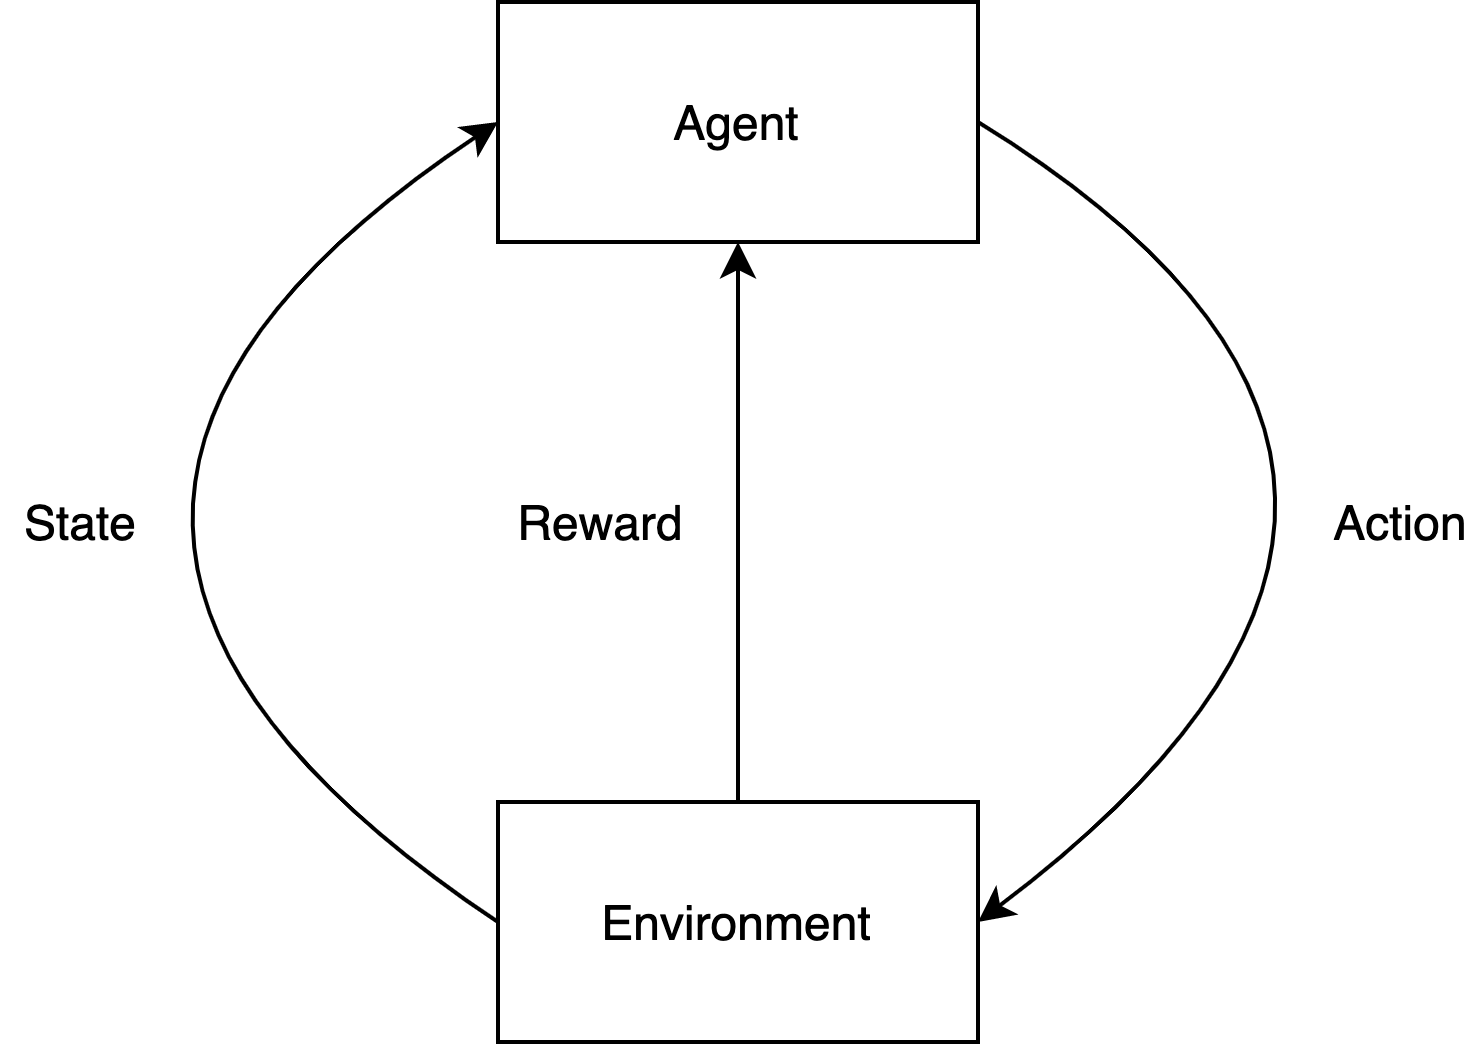
\includegraphics[width=6cm]{./figures/reinforce7.png}
\caption{Reinforcement Learning reward system \protect\cite{sebastiani2002machine}}
\label{fig:RLreward}
\end{figure}
\begin{itemize}
  \item Autonomous Agent: It is the agent's responsibility to take action.
  \item Actions: It can be seen as a set of logical steps which is needed to move forward. An action can be in two states, either reward or penalty.
  \item Environment: This is the environment in which the autonomous agent finds itself.
  \item Reward: The main aim of Reinforcement learning is to obtain rewards, good or bad.
  \item State: Is defined as the position it finds itself in the environment. To move around in the environment, the state needs to keep changing.
\end{itemize}
The goal of an reinforcement learning algorithm is to learn a near optimal policy, that thrives on the rewards system. A policy is the rules of the game. Reinforcement Learning focuses on addressing problems which includes decision making  \cite{Andriybook2019}. This works well for games, robotics and logistics.

\subsection{Supervised Learning}
Supervised Learning (SL) can be defined as a task that is learning the mapping between input and output by looking at examples of the input and output pairs. It creates a model from the labeled training data consisting of a set of training examples. By labeled, it suggests that the mapping between questions and answers, or between input and output has already been done \cite{singh2019natural}.
For example, if we look at a financial company that wants to look at users profiles to decide to give them a loan or not. A Machine Learning model would be trained on historical labeled data, which consists of information regarding profiles of the past customers \cite{kotsiantis2007supervised}.
The methodology that is used in Supervised Learning can sometimes vary based on the output of the model. Some supervised machine learning algorithms are listed here:
\begin{itemize}
  \item Logistic Regression
  \item Decision Trees
  \item Linear Regression
  \item Support Vector Machines
\end{itemize}

Another integral part of Supervised Learning is evaluating the model. Based on the type of model, shown above, the appropriate evaluation metric can be chosen and applied \cite{sebastiani2002machine}. Furthermore, this can be done by splitting the training data into two sets, train set, and validation set. Training of the model would be done on the training set and testing the performance should be done on the labeled validation set. Changes can be made in the Hyperparameters to improve the performance of the model \cite{kotsiantis2007supervised}. Hyperparameters are used to configure various aspects of the learning algorithm and does have a direct impact on the results and the performance of the created model. 

\subsection{Unsupervised Learning}
In Unsupervised Learning, a model is trained on similar unlabeled data. Since the data does not contain labels and sometimes unstructured, the model will just be trained without any influence given by labels. In Unsupervised Learning, the machine tries to find latent patterns and insights into the data that can be used in any form. The relevant Unsupervised Learning algorithms are:
\begin{itemize}
\item Clustering Algorithms (Document and Hierarchical)
\item Dimensionality Reduction Techniques
\item Topic Modeling
\end{itemize}

The rest of chapter \ref{chap: Chapter 3} will cover different applications of unsupervised learning, and how they interact with one another.

\section{Document Clustering}
Clustering is the answer to a problem of learning to map a label to examples based on an unlabeled dataset. Due to the dataset being unlabeled one must decide whether the learned model is optimal, which makes it much more complicated than Supervised Learning. Clustering has several use-cases ranging from text analysis to anomaly detection. A common use-case for businesses is to use machine learning driven clustering for profiling customers based on their activities and building strategies around these results. 

Search engines has been employing clustering by finding similar searches and results in one cluster. Document clustering, a branch of clustering, is the technique data mining uses which includes concepts from fields of Machine Learning, Information Retrieval and Natural Language Processing. Document clustering organizes documents into different groups called clusters, were the documents in the cluster share some common features according to the similarity measure. Clustering in general can produce overlapping clusters or non-overlapping clusters. In an overlapping cluster, it is likely multiple clusters can contain the same document \cite{andrews2007recent}, in a non-overlapping cluster, the opposite can happen. 

An example of supervised learning and unsupervised learning in terms of document clustering can be in document classification, all the classes and their properties are known beforehand. In document clustering, all the properties, or other information are unknown. Thus, classification is an example of supervised learning, and clustering is an example of unsupervised learning \cite{andrews2007recent}.

It can be defined that document clustering can be broken down into two sections, hard clustering, and soft clustering \cite{chen2010integration}. Furthermore, soft clustering can be broken down even more into partitioning and hierarchical.
\begin{itemize}
\item Hard: Clusters the features to exactly one cluster.
\item Soft: Clusters features into multiple clusters. For example: if the papers title needed to be clustered, named "Natural Language and Information Retrieval" would be clustered in both cluster names "Natural Language Processing" and "Information Retrieval".
\begin{itemize}
    \item Partitioning: This type of clustering splits the documents into fixed amount of clusters. An example is K-Means clustering \cite{chen2010integration}. 
    \item Hierarchical: Commonly known as taking shape as a tree of clusters.
  \end{itemize}
\end{itemize}
In this section, we discussed what document clustering is, talking about the different types of clustering. In the next section, the applications of document clustering will be discussed.
\subsection{Document Clustering Applications}
As mentioned above, document clustering falls within supervised learning and can be used in various fields like business and science \cite{jain2010data}. The origin of document clustering research was to improve recall or precision in Information Retrieval (IR) systems, however, recently the application of document clustering evolved drastically.  Document clustering can be applied for example \cite{jajoo2008document,abualigah2017text}:
Firstly, a system which enables people to find similar documents to that what was inputted. Using document clustering enabled systems to find other documents semantically similar \cite{Shah2013}. In recent years, the rate of development in technology spiked research on how to improve document clustering \cite{alhawarat2018revisiting,mekonnen2017topic}. 
Secondly, it is useful to organize large amount of documents in a taxonomy structure.
Thirdly, with the number of documents in the information ocean created a need to find duplicates. Clustering use-cases includes plagiarism detection, identifying related news stories and fake news, and to optimise search engines \cite{jin2016news}.
Lastly, in the most basic form, an academic is recommended papers based on the papers they have already read. This can be done by using clustering and employing other features of the text, and ultimately, improving the quality of recommendations. The use of Latent Dirichlet Allocation and content-based filtering is evident that it can work well as depicted in \cite{yeh2010}.

\subsection{Document Clustering Procedure}
Getting from a collection of documents to a cluster of documents a few processes needs to be followed. The processes comprises generally of three components: 1. feature extraction and selection, 2. document representation, and  3. document clustering \cite{shah2012document}.

Feature extraction takes the document and applies pre-processing steps to it. Cleaning the text includes removal of stop words which should be updated with the domains most common keywords, which would not add any value from a semantic perspective. The document should then be analysed and features should be extracted \cite{mugunthadevi2011survey}. Looking at the extracted features, selecting the right ones would be an important exercise to further remove noise. The benefit is that dimensionality is also reduced by only selecting the wanted features, it helps by enabling better data understanding \cite{wei2006combining}.

After the document has been stripped from all the unnecessary features, the documents are then only left with features which scored the highest in the metric score \cite{Shah2013}. Term Frequency (TF) would be an example of feature selection metrics. The documents are then grouped into clusters based on their features and metric scores which was calculated \cite{wei2006combining}.

\subsubsection{Term Frequency-Inverse Document Frequency (TF-IDF)}
The dataset that will be clustered will be represented as a set of vectors and the vector are called the vector of an object. Vector Space Model (VSM) is an model that represents text documents as vectors \cite{clark2015vector}. 

Term weight value can be defined as the noteworthiness of a specific term in a document. This can be calculated by the number of times the term is occurring within the document over the entire dataset. Term Frequency with Inverse Document Frequency (TF-IDF) is the most commonly used term weight scheme  \cite{cui2005document}. More frequent the words in a document the more important \cite{peng2006recent}.

\subsubsection{Dimension Reduction}

The increase in vast amounts of data has highlighted the inefficiency of most dimension reduction algorithms \cite{mugunthadevi2011survey}. These algorithms are used for feature extraction and feature selection. While feature extraction is taking place, new features are combined with the original features, which causes computation load to increase. In contrast to feature extraction,  feature selection selects the features directly.

\subsection{Similarity Measures for Document Clustering} \label{JSD}

Cluster similarity are based on the measurements between objects. Three main steps are involved to determine the similarity between objects: (1) Identifiers needs to be used to characterize the objects, (2) a weighting scheme needs to be selected, and (3) a similarity coefficient needs to be selected to determine the degree of resemblance between two vectors \cite{willett1988recent}. 

Cluster accurately the precise distance between a pair of objects must be known, in terms of either similarity or distance. Distance and similarity measures has been proposed and used widely, like: (1) Cosine similarity, (2) Jaccard correlation coefficient, (3) Euclidean distance, and (4) relative entropy \cite{huang2008similarity}. An overview of the similarity measures were discussed in \cite{huang2008similarity}.
\begin{itemize}
    \item Euclidean Distance: It is a standard metric for geometrical problems. It is the distance between two points and is the default distance measure used in the K-means algorithm.
    \item Cosine Similarity: The similarity of two documents corresponds to the correlation between the vectors.
    \item Jaccard Coefficient: Jaccard coefficient contrasts the sum weight of shared terms to the sum weight of terms that are present in either of the two documents but not the shared terms.
    \item Pearson Correlation Coefficient: It is an alternative to measure two vectors.
    \item Kullback-Leibler Divergence: Can be used for evaluating the differences between two probability distributions.
    \item Jensen-Shannon Divergence: is based on Kullback-Leibler Divergence with improved differences like, it always returns a finite value and is also symmetric. 
\end{itemize}

Keeping above overview in mind, Jensen-Shannon Divergence has been reported a positive contribution when comparing two probability distributions \cite{Uto2017,9358561}. 

\subsection{Summary}
Document clustering is a crucial fundamental pillar in unsupervised document organization. In this section, we have discussed what document clustering is, the types of clustering used, and the applications that employ document clustering. We later discussed the three phases needed to cluster documents. Emphasizing the importance in extracting and selecting the correct features, which later translates in the quality of clusters. The size of data sets peaked the interest of researchers to look for alternative ways to reduce the dimensions of an SVM. Furthermore, we have also highlighted the types of similarity measures one could use. In the next section, Natural Language Processing (NLP) will be discussed.

\section{Natural Language Processing} \label{secc:LDAover}

Natural Language Processing (NLP) is sub discipline of Artificial Intelligence and Linguistics. The goal of Natural Language Processing was to ease the user's work and to communicate with a computer effectively \cite{khurana2017natural}. Since some of the users are not proficient in machine programming languages, NLP alleviates the pressure that time or lacks the ability to perfect the machine language has on a person \cite{russell2016artificial}. 

A language can be defined as a set of rules or set of symbols \cite{santana2016language}. The symbols can be combined and used for conveying information in a clear and concise manner. This being said, NLP can be classified into two sections: (1) Natural Language Understanding; and (2) Natural Language Generation, which means to understand and to generate text as seen in Figure \ref{fig:CNLP}.

\begin{figure}[htbp]
\centering
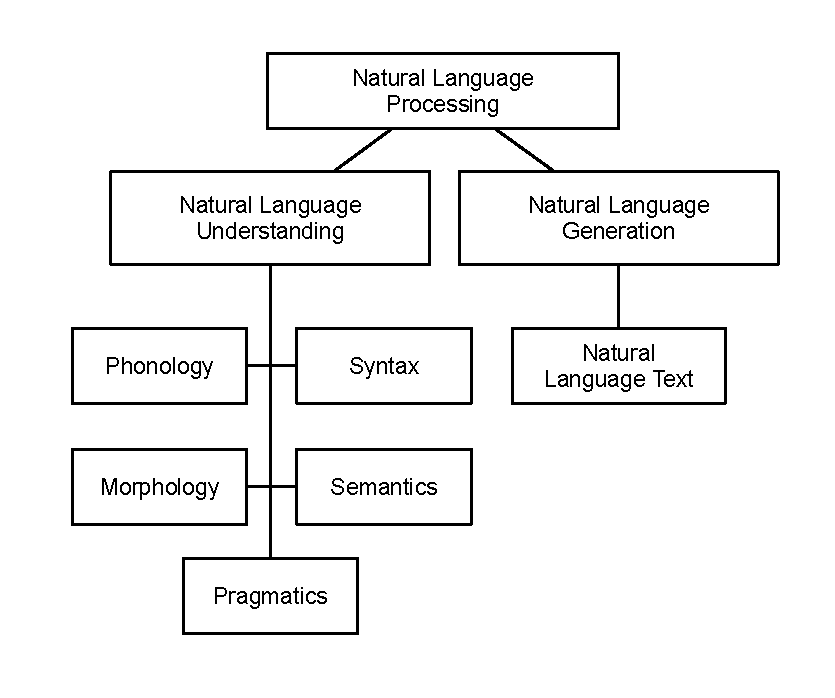
\includegraphics[width=10cm]{./figures/NLP3.eps}
\caption{Classification of NLP}
\label{fig:CNLP}
\end{figure}
Linguistics is the domain in which languages are studied, which involves the meaning of language, and the context language finds itself \cite{Bates9977}. The important terminologies of NLP are: (1) Phonology that refers to the relationship in sound, (2) Morphology word formation, (3) Syntax the sentence structure, (4) Semantics that refers to the arrangement of words and their meaning \cite{hassan2021natural} and (5) Pragmatics which refers to understanding.

To simplify the complexity of Natural Language Processing, it can be broken up into four distinct stages see Figure \ref{fig:stepsnlp}. In a real-world scenario, these stages seldom occur separated. In the overview that follows it is assumed that the syntactic analysis and semantic analysis is done by the pre-processing. The rest of this section contains the processes shown in the figure.
\begin{figure}[htbp]
\centering
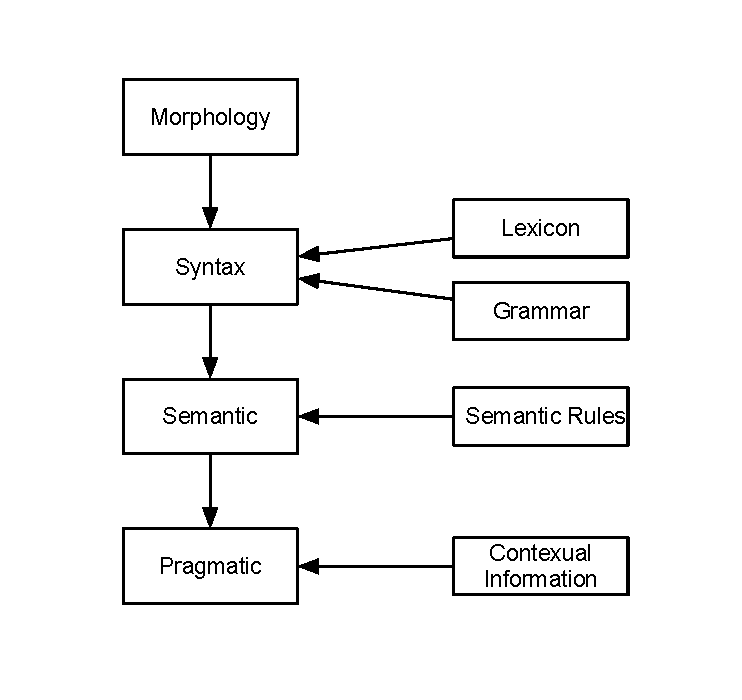
\includegraphics[width=10cm]{./figures/NLPstep.eps}
\caption{Steps in Natural Language Processing}
\label{fig:stepsnlp}
\end{figure}
\subsection{Morphological processing}
The first logical step in a typical NLP system is morphological processing. In this step the text will be broken down into sets of tokens corresponding to the equivalent words, sub-words and punctuation forms \cite{Bates9977}. For example, a word like "unnecessarily" can be broken down into three sub-word tokens: un - necessari - ly.

Morphology can be defined as a study of how words can be modified to have similar meanings but used in different syntax. Modifying these words are typically done by adding prefixes and or postfixes. Generally, word modification can be broken down into three components:
\begin{itemize}
    \item Inflection: words can be represented differently based on the syntax they find themselves.
    \item Derivation: new words are made from existing words. Determines, determining, and determined are from the root determine.
    \item Compounding: new words are made by the grouping of existing words. It is not used so much in English (Example "toothpaste") but is widely used in other languages.
\end{itemize}

Outputs from the Morphology phase is a set of tokens. These tokens can contain identifiable data that is needed for the parser to do it's job. The next stage of processing is syntax and semantic analysis.

\subsection{Syntax and Semantic analysis}

A language processor has certain tasks it needs to perform which is syntax analysis and semantic analysis. There are two main aims for syntax analysis: (1) to check if an sentence is well formed, and (2) to break up the structure to show syntactic relationships between the words. A syntactic analyzer (parser) does this by using a dictionary of words (lexicon) and a set of syntax rules (grammar). The usage of a dictionary and syntax rules indicates how syntactic categories can be combined to form phrases of different types \cite{nation2007dissecting,liddy2001natural,feldman1999nlp}.

This syntax-semantic combination could deconstruct the sentence "The large cat chased the rat" as follows:
\begin{figure}[htbp]
\centering
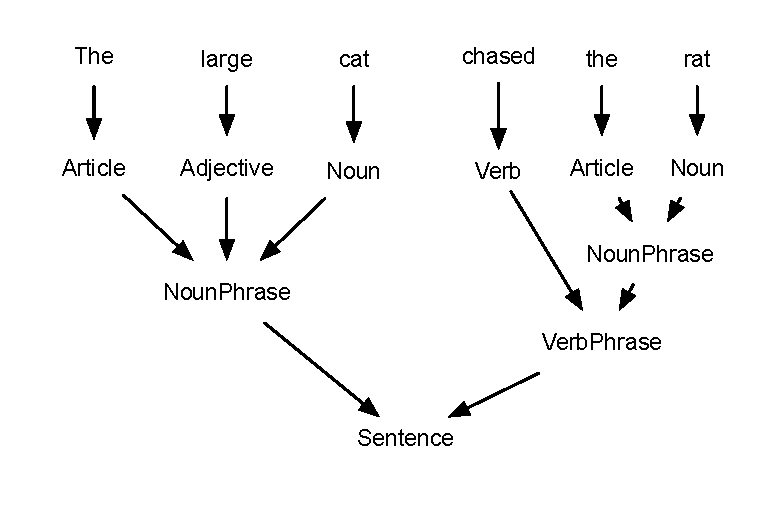
\includegraphics[width=10cm]{./figures/sen.eps}
\caption{Deconstruction of a sentence}
\label{fig:sentence}
\end{figure}
One of the tasks of a language processor is to analyze a sentence and produce a formal notation that concisely expresses the semantics of a sentence and is called Semantic analysis.

When constructing a model, semantic analysis plays the roles of finding meaning of the words in the sentence. In order for that to happen, the dictionary of the model should include weather the words are noun, verb or adjectives. The grammar rule in figure \ref{fig:sentence} with VerbPhrase to Verb, NounPhrase states how the syntactic group is formed.

The important part of this section is to understand that the syntax and semantic analysis phase is of vital importance for any NLP system or tool. The next stage of processing is semantics and pragmatic.
\subsection{Semantics and Pragmatic}

After the combined stages, syntax and semantic analysis, the next stage of processing is pragmatics. There is no clear distinction between semantics and pragmatics \cite{Stern2004}, but for the purpose of this study we make the distinction as follows: semantics studies the meaning of the word and their meaning within sentences whereas pragmatic studies the same word and meaning but within a certain context. Doing semantic analysis on a sentence like "The large cat chased the rat"  can only provide a string of text which translates to the large cat but the identity of the cat. Pragmatic analysis like the example supplied described, simply maps the actual objects which exist in a certain context to a reference obtained during semantic analysis \cite{russell2016artificial}.

This section has provided examples of how analyzing human languages creates certain challenges within the Natural Language Processing domain. In the next section, we will discuss Topic modeling.
\section{Topic modeling} \label{ssec:tmodel}

Language models has recently been used to aid speech recognition and handwriting recognition by showing textual data. Language modeling can be defined as a probability distribution derived from words in an indexed vocabulary \cite{croft2010search}.
\say{They can be used to create new documents by sampling words according to the probability distribution, consider the language model is a pool of words, where the probabilities determine how many occurrences of a word are in the pool, then we can generate word sequences by reaching in, drawing a word, writing it down, putting the word back in the pool and drawing again.} \cite{titov2008modeling}.
This generative process is approximating the model of the topic that the author of the document had in mind when she/he was writing it \cite{raghuveer2012legal}.
A traditional generative model of a language can be used to either recognize patterns of strings or to generate documents \cite{Sajjadi2018AssessingGM}. The generative model as illustrated in figure \ref{fig:automon} as a finite automaton that generates documents.
\begin{figure}[htbp]
\centering
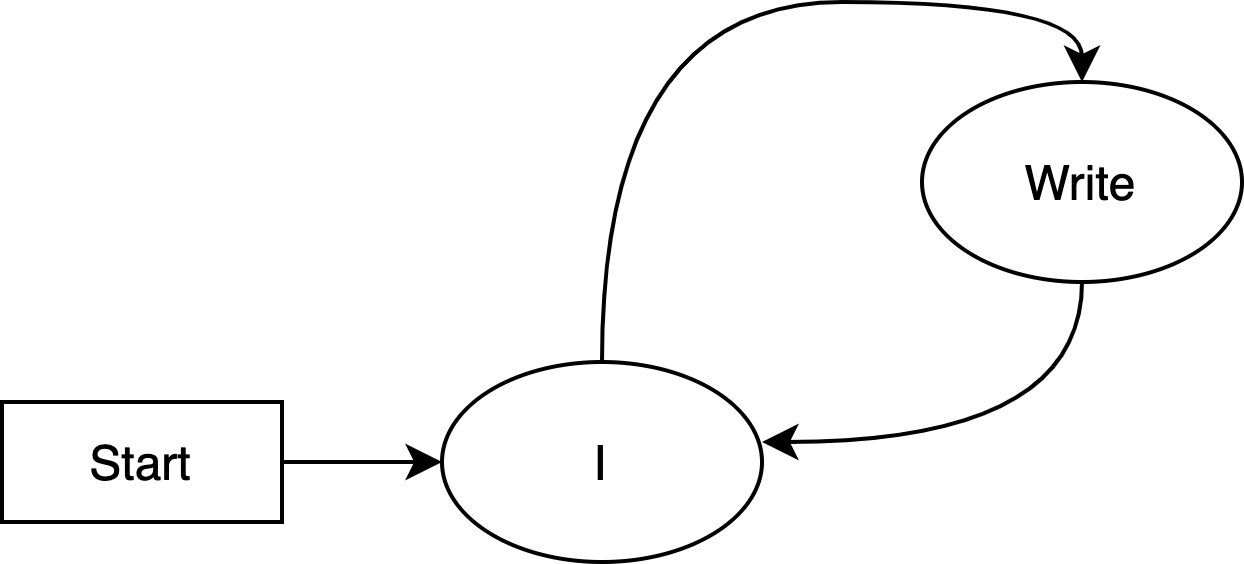
\includegraphics[width=7cm]{./figures/automon8.png}
\caption{A finite automaton and string it generates}
\label{fig:automon}
\end{figure}
Topic modeling has been used as a technique to identify concepts and annotate large text corpora, to keep track of topics over time, and to assess the similarity between topics and  documents. 
The purpose of topic modeling is to analyze data or documents to look for patterns and latent topics. After the topics were identified they would be represented by means of a probability distribution. Topic modeling has been actively applied to several tasks, analysis of scientific patterns  \cite{lau2012line,yi2009comparative,wei2006lda,yi2009comparative}, and scholarly publication search engines \cite{newman2010evaluating}.

Topic modeling is a range of generative models for language that specifies procedures by which documents are built \cite{blei2003latent}. The most preferred algorithm of topic modeling is Latent Dirichlet Allocation (LDA) which describes a generative model for topics and documents \cite{blei2003latent}. 

\subsection{Latent Dirichlet Allocation Algorithm} \label{ssec:LDAA}

Latent Dirichlet Allocation (LDA) is a type of topic model that associates multiple topics for a document. A topic is a distribution over a fixed vocabulary \cite{chaney2012visualizing}. In each topic the distribution of words is different. Assuming the topics are specified before the documents are generated. The documents are generated by the following processes. Initially, the random distribution of topics is selected. For each word in the document a random topic is selected from the distribution of topics. Finally, a word is selected from the topic \cite{blei2003latent,mekonnen2017topic}.

The goal of topic modeling is to discover topics from a collection of documents automatically. To compute the hidden topic structure from documents the probability distribution of the hidden variables given must be computed \cite{mimno2012sparse}.

%\subsection{Use case: Language model and Latent Dirichlet Allocation example}
%To show the process of generating a topic model using the LDA algorithm for a particular document we look at a paper from the ISSA conference corpus. 

%After removing common stop words, we can optionally apply lemmatization or stemming to the corpus. In our example, we only remove stop words since the context of each word or the correct order does not matter. The Bag-of-Words (BOWs) representation will serve as input for our LDA process to generate the LDA model \cite{alghamdi2015survey}.

%In our example, we are using a corpus that consists of 100 papers. This corpus information is needed for smoothing methods that could be applied to the language model. A term not appearing in our paper but in all of the other papers could get a higher probability in the language model than a term appearing in only one paper.

%When applying the LDA algorithm to generate latent topics, we take the BOW representation of all the documents in the corpus. Only the top 10 most likely terms will be displayed. They cover different aspects of Information Security.
\subsection{Topic Model Validation}
The quality, performance and the efficiency of the topic model must be evaluated \cite{ramirez2012topic}. Topic validations have been created to compare the quality of different algorithms. The first approach is to evaluate the topic models based on perplexity, which is calculated on how well the topics were extracted using the training set, and allows to predict the occurrence of words belonging to the training set \cite{ramirez2012topic}.

Other approaches focus on the semantic coherence of the topics. \citeA{chang2009reading} introduced human validation of topical coherence via intrusion tests. The judges had to find the intruder in the evaluated topics and if the intruder was easy detected that means the other words has a strong thematic correlation. However, the process requires manual validation of every build model.
Automatic approaches have been proposed by \citeA{newman2010automatic}, by using Point-wise Mutual Information (PMI) to calculate the co-occurrence in google search results for all given word pairs in the topic. This approach achieved similar results as human coders/judges \cite{alsumait2009topic}.

\subsection{Additional Topic Modeling Tools and Techniques}

Many researchers worked on NLP, building tools and systems which made NLP to what it is today. Tools such as Sentiment analysers, Part of Speech (POS) taggers, Chunking, Name Entity Recognition, Emotion detection and, Topic Modeling. 
A Sentiment analyser works by extracting sentiments about a given topic. Sentiment analysis consists of a topic feature extraction, sentiment extraction and, association by relationship analysis \cite{yi2003sentiment}. Sentiment analysis uses two linguistic resources namely; the sentiment lexicon and the sentiment pattern database \cite{nasukawa2003sentiment}. It analyzes a document for positive and negative words and gives them a rating on a scale of -5 and +5.

Part-of-Speech (POS) tagger can be defined as a piece of software that reads in text and assigns parts of speech to tokens, parts of speech like noun,  verb and adjective. POS tagging is a daunting task because a word can represent more than one speech at different times. Substantially amount of research has been conducted in European languages, and research has shifted to improve POS taggers for other languages like Arabic, Sanskrit \cite{tapaswi2012treebank}, Hindi \cite{ranjan2003part} etc. It can effectively tag and classify words as noun, verb, adjectives, etc. Technological improvements for part of speech tagging can work efficiently on European languages but still lacks advancement on Asian languages \cite{hirschberg2015advances}. The POS tagger used for the Sanskrit language uses the treebank technique \cite{bengoetxea2010application}, Arabic uses the Support Vector Machine (SVM) \cite{diab2004automatic} approach to tokenize, POS tag and annotate phrases in Arabic text.

Chunking is also known as Shadow Parsing, it works by labeling pieces of a sentence with syntactic correlated keywords like Noun phrase and Verb phrase(NP or VP). Each sentence that is being tagged starts with a unique tag marked as Begin chunk (B-NP) tag or Inside chunk (I-NP) tag. Chunking can be evaluated by means of the CoNLL 2000 shared task, which provides test data for chunking \cite{sang2000introduction}. Since the rise of CoNLL 2000 much more systems raised, some reporting around 94.3\% F-Measure score \cite{sha2003shallow,mcdonald2005flexible,sun2008modeling}.

The usage of Named Entity Recognition (NER) in places such as the Internet is problematic because people do not use tradition or academic English \cite{nadeau2007survey}. This brings down the overall performance and quality of language processing tools. By annotating the phrases on unlabeled, in domain and out domain data improves the performance compared to traditional language processing tools \cite{katiyar-cardie-2018-nested}.

Emotion detection is similar to sentiment analysis but used in the social media scene on mixing of two languages (English and one other language). It categorizes statements into 6 different groups based on emotions, namely; sadness, happiness, disgust, fear, surprise, and anger. During the categorizing process, the identification of ambiguous words that are in English + the other language should commence determining the base language of the text. Determining the base language would accelerate the performance and quality of the detection \cite{khurana2017natural}.

Event discovery in social media feeds that uses a graphical model and NER to determine whether it contains the name of a person, city, place, etc. The model operates by listening to noisy data and extracting records and keywords of the events from multiple data streams, despite the noise and the use of irregular language, the model is able to extract records with very high accuracy \cite{benson2011event}. 

\section{Summary}
There has been so much done trying to satisfy the problem of information overload over the past few years that have been using Machine Learning.

In this chapter we discussed why Machine Learning played such a pivotal role in the development in all of these concepts: Document Clustering, Natural Language Processing, and Topic Modeling. 


The next chapter, presents the research methodology that was followed.
\chapter{Research Methodology}
\label{chap: Chapter 4}

As mentioned in the previous chapter, machine learning has many technologies that can be harnessed in easing information overload. However, these technologies should be used in a methodical way.

This chapter provides the reader with information regarding the overall research design and the research methods used.

The following section discusses the research design used. The latter sections discusses how the literature review was conducted and how it can be used for the prototype development. The role experimentation played in the development in the model and prototype.

The following section starts off with the research design followed in the study.

\section{Research design}

This research study has adopted a positivist approach. The positivist paradigm is based on facts and observation \cite{wilson2014essentials} and reduces the impact that the researcher’s interpretation has on the study.

Positivist studies usually come from a deductive research approach, whereas an inductive research approach is manifested within the philosophy of phenomenology \cite{saunders2007research}. The inductive approach can also be known as inductive reasoning, which begins to look for patterns from observations and theories. Moreover, inductive reasoning follows the bottom-up approach, that includes crafting theories or general conclusions from specific observations \cite{saunders2007research}.

For example, when searching for emerging themes in data inductive reasoning is used \cite{Fereday2006}. In contrast, deductive reasoning follows the top-down approach, starting with the general and moving to the specific. It uses facts and rules to arrive at its conclusions \cite{Fereday2006}.

The scientific research domain makes use of this deductive approach. It enables various theories that are tested. Observational hypotheses can be drawn from them and ultimately be compared to data \cite{bechtel2013philosophy}. In the past, scientific research methodologies employed this approach when collecting and evaluating data \cite{MARSDEN2018A1}.

In the next section, the methods that were followed in this research study are discussed.

\section{Methods} \label{ssec:meth}

This research study was primarily experimental in nature. It did not focus on the researcher’s interpretation of the data, but rather on the findings which could be drawn directly from the data. This research study employed a set of methods, which make up the methodology. These methods include a literature review, experimentation, a prototype, and the creation of a model. The upcoming sub-sections provide more detail about how these methods fit into the research objectives and milestones.

\subsection{Literature review} \label{ssec:prep}

A literature review is a process of going through various academic studies in search of information dealing with the topic at hand \cite{olivier2009information}. The literature review in this study focuses on various topics of recommender systems, document clustering, natural language processing and their application to recommend related papers using Information Security South Africa past conference papers. The literature review was conducted to meet secondary research objectives one and two.

\subsection{Experimentation} \label{ssec:exper}

As mentioned, the research took on the positivist philosophy. This study was experimental in nature. As \citeA{olivier2009information} discussed, an experiment can be conducted with the following goals in mind, namely to test a theory, to prove a theory, and to see whether something interesting happens, which is also known as an exploratory experiment.

Experiments have three main goals; they are (1) to explore a theory, (2) test a theory, and (3) prove a theory. It was later added by \citeA{olivier2009information} that it is common for experiments to compare two cases, an older solution to a newer one to see how they compare. In the context of this study, the algorithms and techniques identified were used to construct a prototype to which was used to observe the possibility of using recommender systems, document clustering and natural language processing techniques together to satisfy the primary objective.

Testing can be used to see whether a certain theory holds up against specific cases. In testing a single theory, one should conduct a limited experiment. This may be done to ’feel’ whether the theory is correct, to refine the theory even more, or to justify a full-scale experiment. For example, an academic paper recommender system can employ natural language processing techniques to achieve paper recommendations. If it is determined that the experiment holds true, the theory can either be further refined or a full-scale experiment can then begin. In contrast to testing a theory, proving a theory would be conducted to ensure without a doubt that a theory holds true. Proving the previous theory requires all outside factors, which can be a hindrance, to be removed.

Lastly, to see if something interesting happens. This experimental goal has very little structure and provides freedom to play around with certain ideas. For example, an academic paper recommender system can employ natural language processing techniques along with topic modeling algorithms to achieve paper recommendations. Such experiments do not have certain outcomes and are conducted with no given theory. As mentioned in the previous paragraph, the experiments had little structure and were accompanied by a prototype to maximise what there is to learn. The creation of the prototype and experiments were to satisfy the third research sub-objective.

\subsection{Prototyping} \label{ssec:prot}

In information technology the term prototype refers to a simplified program or system that serves as an example or demo of the full-scale program or system \cite{olivier2009information}. A prototype usually only has a few characteristics of the bigger system. The simplicity of the prototype is deliberate because only the study subject matter will be tested or demonstrated. In the research environment, the prototype research method cannot be used solely to constitute the research. In other words, it cannot be used as the icing on the cake; rather, it needs another method to lean on.

Working well with other methods, a prototype can be used in multiple roles. Commonly, there are four roles that a prototype can take: proof of concept, prototype for experimentation, prototype for conceptual clarity, and exploratory research. First, after proposing and constructing a new model or new concept, researchers build a prototype to prove the concept. In other words, the statement can be made that the concept can be implemented and works well in practice. The second role, prototype for experimentation, can be used to gather all the information about the prototype.

In general, information gathered can range from measuring the speed of the system and the quality of a model. However, measuring the speed or quality of a model alone does not make a big research contribution. The third role, prototype for conceptual clarity, is used when a certain concept or work is difficult to visualise. Developing the prototype with this role in mind forces the researcher to focus on the concepts at hand and helps in not overlooking certain details. Furthermore, after the construction of the prototype and its merit can be shown, it can be used as a proof of concept. Lastly, the final role that a prototype can play is in exploratory research.

In all of the other three roles the prototype is constructed to aid the research process. However, when a model, algorithm or concept is not new there are still lessons to be learnt by developing it. For example, in 2003 a new topic modeling algorithm was created called latent dirichlet allocation (LDA) and it achieved great success in the natural language processing (NLP) and information retrieval (IR) domains \cite{blei2003latent}. However, there were only a few papers available for the use of LDA in the recommender systems domain. This is a perfect example of incorporating LDA into a recommender system to see what lessons there are to learn. If a major issue is identified while constructing the prototype and it can be linked to the incorporation of LDA and recommender systems, this role of the prototype can be used to create new knowledge. The quality of the research will, however, be determined by the interesting data.

\subsection{Modeling} \label{ssec:model}

A model can be defined to capture the essence of the system or process \cite{olivier2009information}. In addition, a model needs to be expressed clearly and concisely. In the context of this study, the model was created as to achieve the primary research objective. The construction of the model commenced after the literature reviews, which satisfied sub-objectives one and two. It then became an iterative process between constructing the model, to build the prototype, and to do experiments on it. The feedback from the experimentation ensured amendments to the model.

Furthermore, \citeA{olivier2009information} states that a model captures the essence or core of a system or process. All of this while it ignores all the aspects that do not bring value. The model in this study was the main method, and the prototype was created to support it. An experiment can be used to validate a model. For example, defining a model that takes academic research papers that learns trends from the academic research papers. The model can be validated by creating a prototype. Where users can look for recommendations based on one of users papers, which the prototype has never seen. In theory, the model looks like it works; however, using an experiment, the model can be tested in practice \cite{Steenkamp2007}.

\subsection{Argumentation}

Argumentation can be seen as the thread which ties several statements together. As mentioned, arguments string from facts to create a premise on which conclusions can be based. An argument can be supported by other arguments, it can derail other arguments, or highlight main ideas \cite{walton2009argumentation}. 

This study used argumentation throughout the development of the model. Deductive argumentation was used to develop a theory to create and test a high-level model, diving deeper into which algorithms were needed to address the primary objective.

\section{Summary}

This chapter has discussed two major points: (1) the paradigm in which the research finds itself, and (2) the collection of methods which the study employed to achieve the main research objective. The aim of the research was to explore the possibility of using natural language processing and information retrieval techniques to satisfy the research objective; thus making it an exploratory study.

The literature reviews reported on in Chapters \ref{chap: Chapter 2} and \ref{chap: Chapter 3} showed viable avenues and options to pursue. This finding ensured that the model would be based on pre-existing knowledge, establishing it in the domain of epistemology. The second half of the chapter covered the different methods used. A survey of the literature to identify trends and algorithms that could be used in the study was captured in Chapter \ref{chap: Chapter 3}. This was followed by creating a prototype of the proposed model and running various experiments with it, adjusting certain values every time.

In the next chapter, the construction of the conceptual model will be discussed.

\chapter{Conceptual Model}
\label{chap: Chapter 5}

In Chapter \ref{chap: Chapter 2}, we discussed a brief history and introduced the three main types of recommender systems. The importance of this exercise was to review the literature and to determine the inner workings of how recommender systems work. The corpus of papers revealed that nearly 55\% of papers employed the content-based filtering (CBF) techniques of handling the content and the ranking system i.e., user profile building. This led to further exploration to find algorithms and techniques that will complement CBF.

Chapter \ref{chap: Chapter 3} lay the groundwork and introduces various machine learning (ML) technologies. Primarily, the literature in Chapter \ref{chap: Chapter 3} was reviewed to shed a light on the field of machine. However, it introduced complex interrelationships within its domain and the interaction with others. These interrelationships created the need to identify and approach employing various technologies covered in Chapters \ref{chap: Chapter 2} and \ref{chap: Chapter 3}.

In Chapter \ref{chap: Chapter 4}, the approach was not only set out, but various stepping stones also were discovered. The creation of the initial prototype was discussed in this chapter. Furthermore, common traps and concerns were identified, i.e. feature extraction, selecting the number of topics, and the technology used to determine the similarity or to recommend academic papers.
In this chapter, the recommendation model, a conceptual model is developed to ease the intricacy surrounding the implementation of a NLP based recommender system. 

The recommendation model uses various algorithms and techniques derived from Chapters \ref{chap: Chapter 2}, \ref{chap: Chapter 3}, and \ref{chap: Chapter 4}. In Section 5.1, the model will be discussed from a birds-eye view. Later in the chapter, we will transition from an abstract level to a slightly more technical one. The above-mentioned technical overview will be covered in Section 5.2.

\begin{figure}[htbp]
\centering
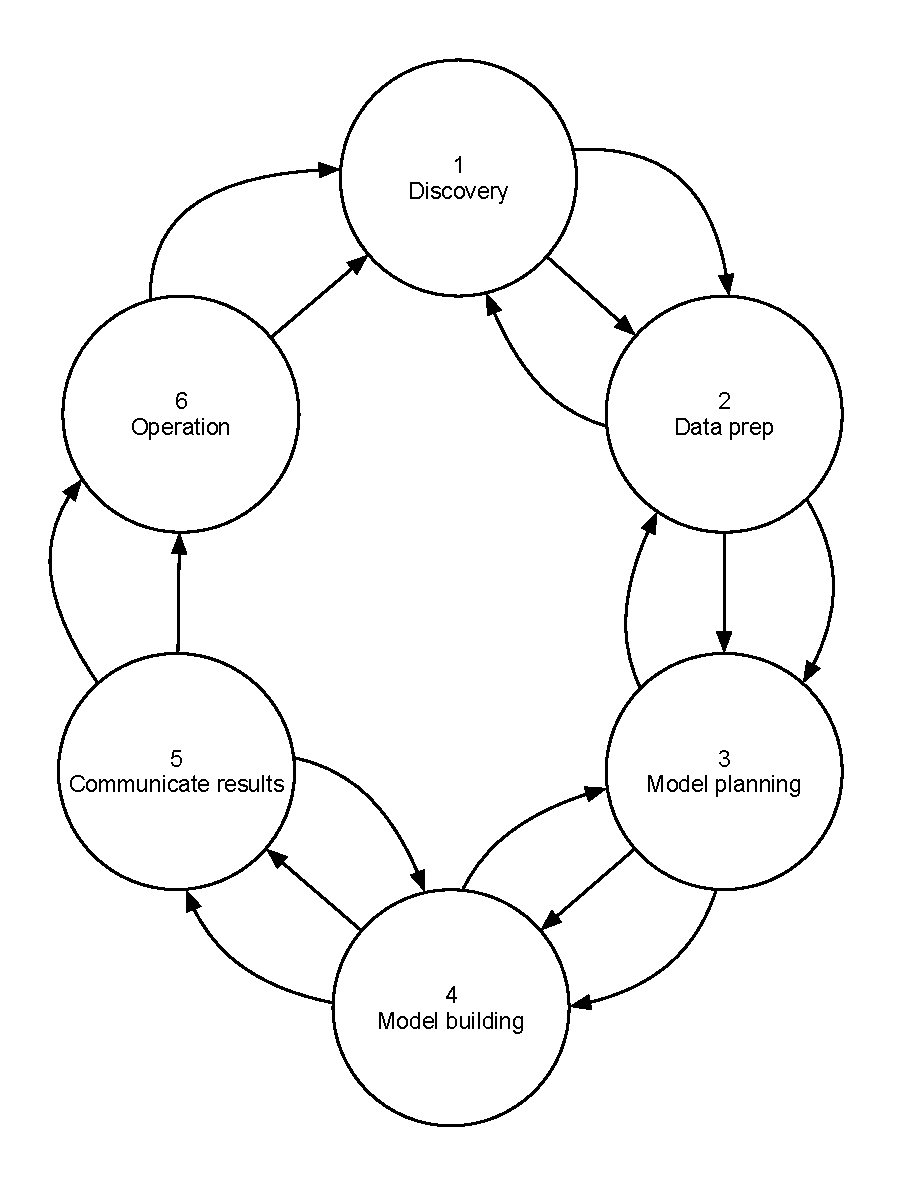
\includegraphics[width=8cm]{./figures/datalifecycle.eps}
\caption{Data Analytics lifecycle}
\label{fig:lifecycle}
\end{figure}

\section{Model Overview}

In recent years, research and development have been focused on creating a streamlined, widely acceptable data analytics lifecycle.

The goal of the data analytics lifecycle was to have a structure in place that could aid developers and other researchers. Teams usually learn new things throughout their projects and often need to go back to the previous phase to refine their work based on new insights and information they have uncovered \cite{dietrich2015data}. 
Each component of the data analytics lifecycle will briefly be discussed below:

\begin{enumerate}
    \item Discovery – in this phase, discovering and gathering data is undertaken. It is essential to frame the data needs best and to obtain the correct data according to the requirements.
    \item Data preparation – the data must be correctly formatted to be used in a later phase.
    \item Model planning – this phase entails looking at various methods, techniques, and workflows that need to be employed to learn about the underlying relationships between the variables.
    \item Model building – also known as analyze data, this phase focuses on analysing the data and determining whether the existing tools will suffice to get to the end goal.
    \item Communicate results – in this phase, various visualisation techniques will be considered and a summary will be developed to convey to the stakeholders.
    \item Operationalise – this is also commonly known as making decisions. This phase focuses on delivering reports, code, and other technical documents.
\end{enumerate}

\begin{table}[htbp]
\centering
\begin{tabular}{|l|l|l|}
\hline
\textbf{Known terminology} & \textbf{Study terms} & \textbf{Domain of techniques} \\ \hline
Discovery & Past papers & Dataset\\ \hline
Data prep & Preprocessing & Machine learning - Chapter \ref{ssec:prep}\\ \hline
Model planning & Learning & ML + IR - Chapter \ref{chap: Chapter 3} \\ \hline
Model building & Human intervention & Prototype - Chapter \ref{ssec:prot} \\ \hline
Communicate results & Represent in data frame & Discussion - Chapter \ref{chap: Chapter 7}\\ \hline
Operation & Enable decision makers & Evaluation - Chapter \ref{ssec:eval} \\ \hline
\end{tabular}
\caption{Mapping between Terminologies Used in the Study}
\label{tab:mapping}
\end{table}

\begin{figure}[htbp]
\centering
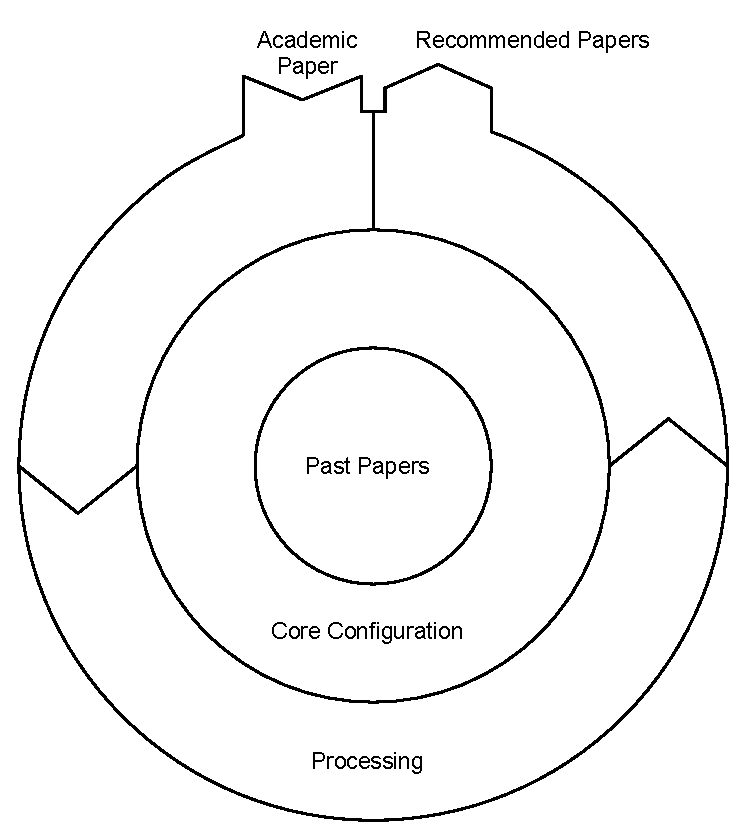
\includegraphics[width=8cm]{./figures/overview3.eps}
\caption{The Model Overview}
\label{fig:Modeloverview}
\end{figure}

With the above being said, the researcher felt the need to provide a mapping between the terminology used in the research domain and this study. As seen in Figure \ref{tab:mapping}, it should be known that when the researcher uses terminology like past papers, pre-processing, and learning they hold the exact content of the corresponding terms used in research. The column on the right in Figure \ref{tab:mapping} can be translated to be the domain and/ or section in this study which addressed each phase of this model.

This section of the chapter covers the model overview, as seen in Figure \ref{fig:Modeloverview}. The model is categorised into three components: (1) past papers, (2) learning, and (3) processing.

Past papers can be identified as the core of the model. It is made up of past or historical papers. This will then flow into the learning component, which is a fundamental stepping stone in defining what needs to be done. In the processing component, the model looks at the defining functions in learning and further refines them. The learning and the processing component will be discussed further in this chapter.

\section{Learning}

The learning component is created by analysing past papers closely. The goal was to understand better the characteristics which made up the learning component. The conceptual model is constructed in such a way that it is not only information security domain-specific. This being said, the characteristics of the learning component were identified and guided by literature. The characteristics of the learning component are:

\begin{enumerate}
    \item Populating the stopword list
    \item Stemming
    \item Topics of the model
    \item Measuring the similarities
\end{enumerate}

\begin{figure}[htbp]
\centering
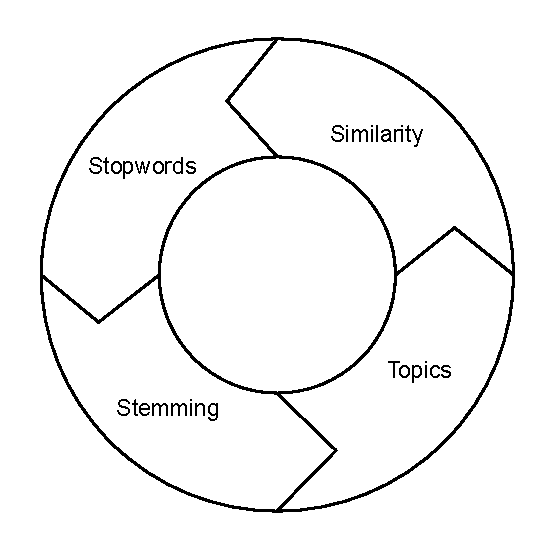
\includegraphics[width=8cm]{./figures/learning.eps}
\caption{Learning Component}
\label{fig:core}
\end{figure}

The flow of the learning component is using the stopword list, then stemming those words. Stemming leads into topics that will be generated, and the similarity of these topics will be measured. As seen in Figure \ref{fig:core}, the flow of the learning component  leads one character into another. The reason for this is that the learning component is a continuous process. Each of these characteristics is described in the following sections.

\subsection{Populating stopword list}

The stopword list was primarily made up of NLTK’s stopword list. The goal of this choice was to employ a stopword list with a comprehensive list of words. NTLK is one of the most widely used NLP libraries. Furthermore, after close consideration, additional words were included in the stopword list as time passed. These words were primarily domain-specific such as: (1) information, (2) technology, and (3) security.

The goal of the inclusion was to retrieve second- or third-tier topics from the text. The textual outputs of each component of the learning component were analysed, and words that did not bring any value or primarily domain-specific words were omitted.

The process of including some words and excluding others was a manual and iterative process. The resulting words were best suitable for the information security domain and were used as the stopword list.

\subsection{Why Stemming?} \label{ssec:stemming}

Stemming was employed for the sheer simplicity and thorough work it has done. To recap, stemming is removing the suffix of the word to return it to its root form. The Porter stemmer is appropriate to IR research work involving stemming where the experiments need to be repeatable exactly. This being said, after consulting the dataset, it was identified that the domain in which this research position found itself did not need to have a custom-made stemming solution.

After close consideration, the researcher, along with evidence, used Porter stemmer from the NLTK library.

\subsection{Topics of the model}

The information technology domain is such a rich field with regard to topics and sub-topics. It needed to be scoped down to provide better topics for the algorithm to use. For example, information, technology and security would be excluded. As seen in Section \ref{fig:core}, all of the components fed into one another. In this case, specific topic names were appended in the stopword list. 

The result of the methodology mentioned above was smaller topics. These were second- and third-tier topics, such as hacking and man-in-the-middle attacks, respectively. A few of the lower-tier topics fused to make up the second-tier topics. This also holds for second-tier- and first-tier topics.

\subsection{Measuring the similarities}
The vast number of topics made it challenging to group similarities of papers. The topics were too dense from the perspective of dimensionality. For the scope of this research, similarity algorithms reduced dimensionality. In addition to the dimension reduction, the unsupervised learning approach made it viable to use an algorithm to cluster similar topics. This would have a direct impact on measuring the similarities in the academic papers.

\subsection{Learning component summary}

There are four components to the conceptual model. They were discovered by reviewing literature and by building a proof of concept. The first component on the list, stopword removal, was fundamental in getting the text ready for further analysis. The stopword list was compiled by using the standard NLTK stopword list and adding a few first tier information security topics, to reduce scope.

The second component, stemming, removed the suffix of certain words to take them to their root form. For the third component, topics, the corpus exists of various tiers of topics. A collection of specific tier topics would form a topic in a higher tier. The similarity between these topics would then be calculated to reduce dimensionality and to cluster most similar topics together.

\section{Processing}

In this section, the next phase of the conceptual model will be discussed. The academic paper processing phase is executed when a new and unseen academic paper is submitted. Just like the learning component, this phase also has four components. It is merely an extension of the components found in the learning component.

In the first step, the fundamental stepping stone was actioned, the removal of stopwords. The new document had its stopwords removed to simplify and get the text ready for further analysis. Step two includes taking the text that was cleaned and stemming it. This removed the suffix and returned the words to their root form. The goal of Step three was to get the related topics in the text. The last step, Step 4, focused on using the topic output and determining the similarities of the topics. These four components are best described in Figure \ref{fig:processing}, and a brief description of each component is given in the following sub-sections.

\begin{figure}[htbp]
\centering
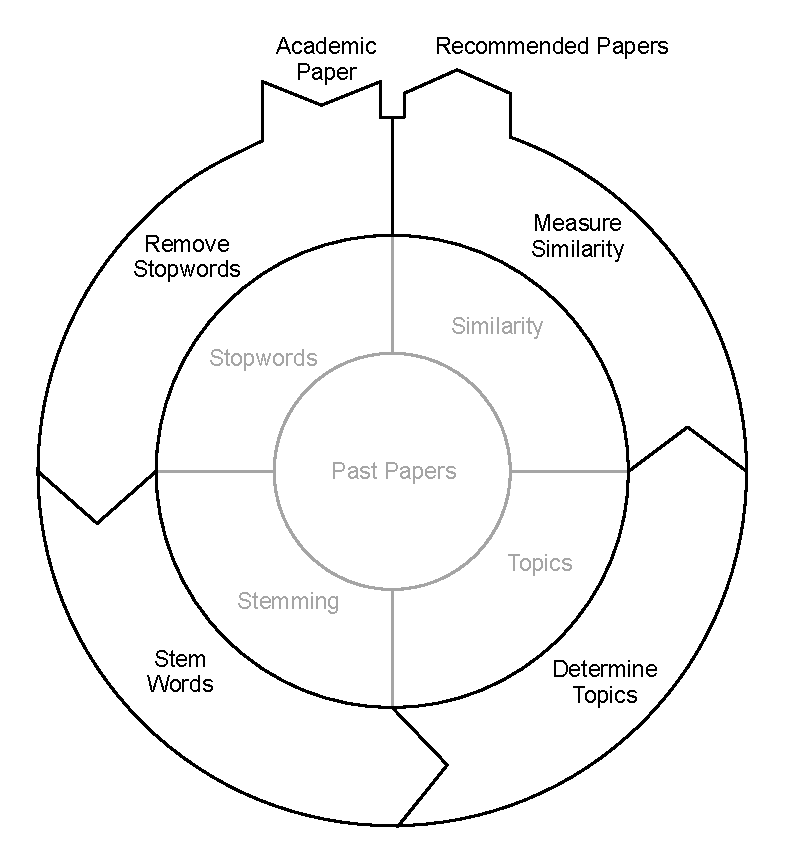
\includegraphics[width=8cm]{./figures/processing1.eps}
\caption{Processing phase of the model}
\label{fig:processing}
\end{figure}

\subsection{Removing the stopwords}

The stopwords are removed from the collection of documents. The goal was to remove the words that do not bring any meaning to the sentences. These are terms such as ’specified’ , ’specify’, ’specifying’. The stopword list also included words such as ’information’, ’security’ and ’technology’.

\subsection{Stemming of the words}

After the stopwords were removed, the tokenised dataset was then stemmed. For example, the words mentioned above: ’specified’ , ’specify’, ’specifying’ can be stemmed and will look like the following: ’specif’, ’specif’, ’specif’. As explained in the learning component section of this chapter, stemming is removing the suffix of the word to return the term to its root form. The stemmed words are then used to determine topics.

\subsection{Determining the topics} \label{ssec:topic}

This component comprises determining the topics of the dataset. This is done after the stopwords were removed and after the text was stemmed.
A topic modeling technique was then applied to the dataset after it was transformed. The soft clustered topics looked something like this: ’0.040*”data” + 0.033*”file” + 0.024*”encrypt” + 0.021*”cloud”. A similarity ratio of the terms was calculated, and the most similar terms were clustered together, forming topics.

\subsection{Measuring the similarities}

At this point of the conceptual model, the stemmed words that did not contain any stopwords were pushed through the topic modelling technique. The product of the previous three components was a collection of topics that represented the dataset. The collection of topics of the dataset and the topics of the test set were measured in terms of similarity. The lower the score, the more similar the two papers were with one another.

\subsection{Processing phase summary}

In this section, we discussed the academic paper processing phase. This phase was executed when a new document was submitted. The dataset already removes the stopwords, stemmed, and determined the topics. Once a new document was submitted, it went through the same process. The only difference there was that the similarity of the two datasets were then measured. The topics with the lowest score were most similar.

\section{Conclusion}

The conceptual model presented in this chapter is a template for finding similar academic papers. The use case for this research was focused on information security academic papers. However, it can be used to find any academic papers across disciplines. The conceptual model was built on a collection of academic papers or datasets. Various learning components were identified while surveying the field. The learning components were broken down into four distinct components: (1) stopword, (2) stemming, (3) topics, and (4) similarity.

After the learning component was built through experimentation, it was ready and waiting for new academic papers to do the testing. The academic paper processing phase could then begin. Just like the learning components, the academic paper processing phase also has four components.

First, the dataset was cleaned of all the stopwords. Special consideration was made for the first-tier topics like ’information’ and ’security’, and those were also included in the stopword list.

Second, once the stopwords were removed, next would be to stem the remaining data. Stemming commonly includes omitting the suffix of a word. This was done to return the word to its root form.

Third, topics were determined by using a topic modelling technique. The technique helped soft cluster all of the similar terms together, which formed topics. These topics consisted of the ’training set’ corpora. Once a ’test set’ document appeared, it was run through the same components.

Once we had the ’training set’ and ’test set’ ready, the last component measured the similarity between the two sets. The new, unseen ’test set’ document was then hard clustered to the most similar set of topics. In the next chapter, the prototype development will be discussed.

\chapter{Prototype development}
\label{chap: Chapter 6}

Chapter \ref{chap: Chapter 5} introduced the conceptual model. This chapter will discuss everything that is needed to develop the prototype and performing the experiments. The prototype essentially provides an implementation of the conceptual model defined in Chapter \ref{chap: Chapter 5}.

\begin{figure}[h!]
\centering
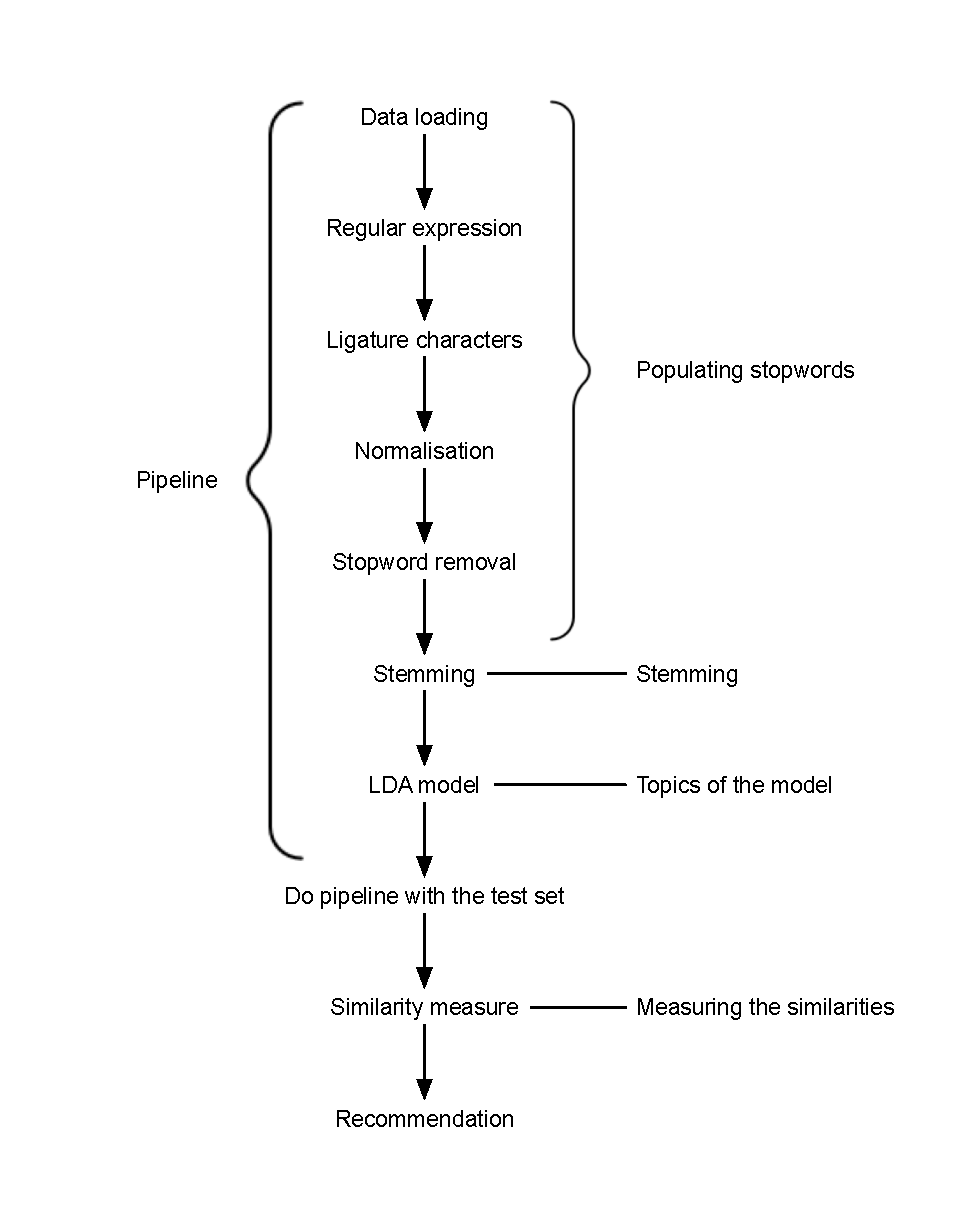
\includegraphics[width=12cm]{./figures/flowresearch12.eps}
\caption{High level overview of the prototype}
\label{fig:prototype}
\end{figure}

The rest of the chapter will look at each element in the pipeline, as depicted in Figure \ref{fig:prototype}, especially with the focus on the refinements that were applied. Figure \ref{fig:prototype} illustrates the steps that were followed in the creation of the prototype. Furthermore, Figure \ref{fig:prototype} shows mappings from the prototype development and refinement to the various parts which were created in the conceptual model chapter, in Chapter \ref{chap: Chapter 5}. In addition, the parts that were intentionally neglected will also be discussed. This chapter will start with a overview of the development of the prototype.

\section{Prototype overview}

The prototype can be split up into four parts at a system level view: (1) identification and removal of the stopwords, (2) stemming the text, (3) topics of the model, and (4) similarity measurement between the test and training set. Although the identification and removal of stopwords and stemming can be grouped under pre-processing, it is important to note that each has an important role in the development of the prototype. Each part plays a critical role in how usable the text is for further topics modeling. Stopword identification and removal is a process that is applied the same in the learning phase and testing phase of the prototype, the same goes for stemming.

As mentioned in section \ref{ssec:model}, it is utmost important to develop a prototype to validate a model. There will always be lesson to be learned, which will be discussed in chapter \ref{chap: Chapter 7}.

The prototype was developed to achieve the following goals:

\begin{enumerate}
    \item To better understand the problem domain, the research problem, and the solution.
    \item To show that the natural language processing and topic modelling approach is feasible.
    \item To be used in recommending research papers and to see the relevance of those recommendations made from the prototype.
\end{enumerate}

The prototype has undergone three iterations, which have supported the goals stated above. The first iteration tied in with the first goal, to better understand the domain and to explore a possible solution. The first iteration provided insight by exploring how recommender systems work and the techniques employed to achieve the desired goal. The second iteration focused more on the initial pre-processing phase of the prototype along with the topic modeling algorithm, latent dirichlet allocation (LDA), and what is to be learned from the development. The topics were later analysed to assess whether this approach will be sufficient. Lastly, the third iteration of the prototype was more polished and had refinement applied to it. The focus shifted slightly from NLP and topic modelling to better the quality of the recommendations made by the prototype. Throughout the third iteration, several parameters in the LDA algorithm were changed to better the recommendations. Unless specified otherwise, reference to the prototype will imply the usage of the third iteration of the prototype.

The researcher decided on Python as the base development environment. Python is a programming language that has gained its popularity in recent years for its modularity and effectiveness of handling data. Many developers have built various libraries in aiding the machine learning and information retrieval community with better system building.

More specifically, the researcher used Jupyter Notebook to build and test the prototype. Jupyter Notebook is a web application, which provides a Python development environment for users. Jupyter Notebook can be used in various ways: data cleaning, data transformation, statistical modelling, data visualisation and machine learning. It allows you to create and share documents that contain live coding, visualisations, and text, thus making it perfect for reproducability of the prototype and making the experimentation easier.
Every part of the prototype will now be discussed along with the various components related to each part.

Code snippets were used from:

%\href{https://github.com/JuandrevanHeerden/Brix-M-Final-Draft/blob/5b287c20b63be6e64b5cc1f4d8b5101bbc92559e/Brix%20M%20final\%20final\%20final.ipynb}{Something Linky}


\section{Identification and removal of stopwords} \label{ssec:pre}

More frequently than not, looking for papers and analysing them is a daunting task for most researchers. The problem is that those papers found by researchers have too much noise to do the necessary, thus creating the need to clear all the unwanted noise from the text. One of the processes within pre-processing is called stopword removal.

Pre-processing contains many techniques to clear the text and make it ready for analysis. These techniques are primarily used in text mining pipelines to better the text input into Information retrieval systems. These techniques include tokenisation, stopword removal, and stemming and transforming the data into a vector space later in various text mining algorithms.

Before stopwords can be removed, they first need to be identified. Each document that needs to be pre-processed contains domain knowledge that is not shared across other domains. Specific domain knowledge needs to be identified first, and then certain words need to be applied to the stopword list. First the data needs to be extracted and analysed. In the next sub-section, we will discuss how the data was extracted. After that, we will discuss the steps taken to identify domain-specific words and add them to the stopword list.

\subsection{Extracting the data}

The data used in this study was obtained from the International Information Security South Africa Conference website. The articles were downloaded and documented in a per year fashion. Furthermore, the abstracts along with the title of each article were manually extracted into the form of ten csv files as seen in figure \ref{fig:github}. Each csv file had two columns named \textit{title} and \textit{abstract}.

\begin{figure}[h!]
\centering
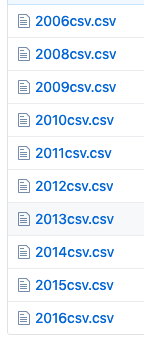
\includegraphics[width=2cm]{./figures/github.png}
\caption{Data on Github}
\label{fig:github}
\end{figure}
The collection of csv file were uploaded to github for documentation and reproducible purposes. A python library called Pandas was used to handle the data as seen in figure \ref{lst:data}. Pandas is a well known library which is primarily used to manipulate data. 
\begin{lstlisting}[language=Python, label={lst:data}, caption=Importing data to the system]
# Import Dataset
df = pd.read_csv('https://raw.githubusercontent.com/brix-mix/Fake/master/2006csv.csv', usecols = ['abstracts','title'])
df1 = pd.read_csv('https://raw.githubusercontent.com/brix-mix/Fake/master/2008csv.csv', usecols = ['abstracts','title'])
frames = [df, df1]
df = pd.concat(frames, ignore_index=True)
df.head()
\end{lstlisting}
The dataset consists of 254 documents spread over 10 years. As shown in figure \ref{fig:data}, the largest document has 235 words whereas the document with the least number of words are 10. The average number of words in the documents are 110, what this means is that there are around 20 percent of the words that will actually have meaning. Usually, out of 100 words used in a piece of writing 20 are of meaning, the rest are filler words or stopwords.
\begin{figure}[h!]
\centering
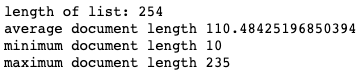
\includegraphics[width=6cm]{./figures/docstats.png}
\caption{Statistics of the documents}
\label{fig:data}
\end{figure}
It is best practice to remove all the stopwords and unwanted characters from your dataset. Junk-in equals junk out. In order to achieve good results, a decision was made to clear the text from unwanted characters. The next sub section includes further removal of unwanted text.



The data used in this study was obtained from the International Information Security South Africa Conference website. The articles were downloaded and documented in a per year fashion. The abstracts, along with the title of each article, were manually extracted into the form of ten csv files as seen in Figure \ref{\ref{fig:github}}. Each csv file had two columns named title and abstract. 


The collection of csv file were uploaded to github for documentation and reproducible purposes. A Python library called Pandas was used to handle the data, as seen in Figure 6.1. Pandas is a well known library, which is primarily used to manipulate data.





\subsection{Regular expressions}
Regular expression can be seen as a sequence of characters that can be used to search for patterns, and those patterns are used to find and replace those characters. The nature of the domain of the document suggests that email addresses and other unconventional characters could be found in the text, therefore figure \ref{lst:re} was used to remove these characters.
\begin{lstlisting}[language=Python, label={lst:re}, caption=Regular Expression]
text = re.sub("((\S+)?(http(s)?)(\S+))|((\S+)?(www)(\S+))|((\S+)?(\@)(\S+)?)", " ", text)
\end{lstlisting}
This code segment was only running once because all data was already in one big data frame. Looking at the raw text, the researcher found ligature characters which was also needed to be removed and replaced. In the next sub section more details were discussed.

\subsection{Ligature Characters} \label{ssec:ligature}

In writing or typography, two or more characters can be merged into one to form; a glyph or single character called a ligature. Ligature characters were commonly used in \TeX{}. \TeX{} is a formatting system that was created and made famous in academia. The ease of executing specific typesetting tasks gave \TeX{} its popularity. 

This research dataset contains older papers published in 2006 onward, making it ligature prone. The two ligatures that were found in this research were; fi and fl. The main reason to replace these ligatures is to normalize the text, so readers that do not change their font encodings can have no problems reading it.
As seen in Listing \ref{lst:ligature}, the use of regular expressions were employed to find and replace the ligatures respectively.
\begin{lstlisting}[language=Python, label={lst:ligature}, caption=Replacing Ligature Characters]
    # Remove fi and fl ligature characters
    text = re.sub("fi", "fi", text)
    text = re.sub("fi", "fl", text)
\end{lstlisting}
After removing the ligature characters, the normalized, tokenized text is ready for the stopwords to be removed.

\subsection{Stopword Removal}
A stopword can be defined as a word that is commonly used within a sentence. However, stopwords in this study are standard Information Security terms that need to be filtered out to enhance the quality of the topics. This was a delicate tweaking process. Only after the data was tokenized and viewed by the researcher a call was made to include several terms. The additional terms that was added was appended to the stopword list as seen in Listing \ref{lst:stopword}, the total number of stopwords totaled up to 282. After the filler words were excluded from the corpus, the next step in the pipeline is to stem the words.
\begin{lstlisting}[language=Python,label={lst:stopword}, caption=stopwords code]
stop_words = stopwords.words('english')
stop_words.extend(['used','using','jam','found','plays','information','security','network', 'technology', 'bgp'])
\end{lstlisting}

\section{Stemming}
As mentioned in chapter \ref{ssec:stemming}, the Porter stemmer is used in the research \cite{porter1980algorithm}. The goal of a stemmer is to reduce the forms of a word to the common base word. Stemmers usually cuts off the end part (affixes) to achieve above goal. 

Stemmers are easy to implement and do not need the time or resources to complete the task. This research looked at high performance, low time, or resources spent on normalization of words. Stemming was selected to be used in this study based on the simplicity and time it takes.

In the below listing \ref{lst:stemming}, we display the code snippet of how the stemmer was used.

\begin{lstlisting}[language=Python, label={lst:stemming}, caption=Stemming the corpus]
stemmer = PorterStemmer()
def stem_words(text):
    """
    Function to stem words, so plural and singular are treated the same
    """
    try:
        text = [stemmer.stem(word) for word in text]
        text = [word for word in text if len(word) > 1] #make sure we have no 1 letter words
    except IndexError: # catch the exception
        pass
    return text

\end{lstlisting}

In listing \ref{lst:stemming}, the core code was to instantiate the Porter stemmer and feed the data through it. We also encountered that some words like 'eod' broke this and needed to insert a try catch, to make the code continue running. 

\begin{table}[htbp]
\centering
\begin{tabular}{|l|l|}
\hline
\textbf{Word} & \textbf{Stemmed word} \\ \hline
informational & inform \\ \hline
translations & translat \\ \hline
evaluating & evalu \\ \hline
itemization & item \\ \hline
awareness & awar \\ \hline
reference & refer \\ \hline
plotted & plot \\ \hline
\end{tabular}
\caption{Stemming words from the data}
\label{tab:stemming}
\end{table}

Some of the words that was found in the data along with their root forms can be viewed in table \ref{tab:stemming}. The Porter stemmer takes the original word back to it's root form.

In the next section, getting topics for the model will be discussed.

\section{Topics for the model}
This section will be a in depth continuation from chapter \ref{ssec:topic}. The bag of words was the step  taken between normalising the data and feeding it into a topic modeling algorithm. Later in this section, the topic modeling technique and its parameter refinement will be discussed.

\subsection{Bag of Words}
For the topic modeling techniques to compute the latent topics, it needs to understand the document. Before the text gets to the topic modeling technique, the text is just tokenized and normalized. Thus, creating the need to represent the text in a manner, the topic modeling technique can interpret it. The most common technique in Natural Language Processing and Information Retrieval is the Bag of Words (BoW) model.

The Bag of Words (BoW) model can be used to extract features from the text. A BoW model is a way to simplify the representation of words in a document. Note that it is called a 'bag of words', the order of the words or sentence of the words does not bear merit. The BoW model is only interested in known words in the document, and the rest is discarded. \citeA{goldberg2017neural} mentions that documents are similar if they have similar content. The BoW model can be simple to use or rather complex by determining the vocabulary of known words and how to score the reoccurring words. 

Determining the vocabulary will be shown below.
Below are snippets from a paper dealing with Phishing attacks occurring through email and social networking sites. Each sentence will be handled as a document. Ignoring case and punctuation, the sentences are:
\begin{itemize}
    \item Phishers continuously seek new methods... 
    \item Conducting phishing solely through email...
    \item Social network phishing and discusses...
\end{itemize}
After removing stopwords. The unique words here are:
\begin{enumerate}
    \item "Phish"
    \item "Method"
    \item "Conduct"
    \item "Email"
    \item "Social"
    \item "Network"
\end{enumerate}
This is a vocabulary of 6 words from a corpus of 15 words. 
Scoring the words can commence once the vocabulary has been selected. There are two scoring approaches one can follow. They are;
\begin{enumerate}
    \item Counting the number of times the word is being used in the corpus.
    \item Frequencies can be calculated by how frequently each word is used out of all the other words.
\end{enumerate}
This research employed the first scoring approach by counting the words. A library called Gensim with a function of doc2bow was used to count the number of times the word occurs, converts the word to a word id and then returns the result as a sparse vector \cite{rehurek2010software}. 
Scoring the previous three documents against the vocabulary of 6 words will look as follows:
\begin{lstlisting}[language=Text, label={lst:scoring}, caption=Scoring the documents]
    Phishers continuously seek new methods = [1, 0, 0, 0, 0]
    Conducting phishing solely through email = [1, 1, 0, 0, 1]
    Social network phishing and discusses = [1, 1, 1, 0, 0]
\end{lstlisting}
Each sentence in listing \ref{lst:scoring} was compared to the tokenized and normalized list. 
In conclusion, the BOW model dis-regards context, the meaning of the words and lastly, the order which the words appear. Thus gives the BOW model its strength because the more similar  words are, the more similar documents are to each other. In the next subsection, we will be discussing how the vector (BOW) is used in the topic modeling technique.

\subsection{Topic modeling parameters} \label{ssec:LDA}

In chapter \ref{chap: Chapter 3}, this study discussed what Latent Dirichlet Allocation is and how it works. In this section we will discuss how the LDA algorithm parameters works on a deeper level. It should be said that in Latent Dirichlet Allocation order of the words do not matter, because of the Bag-Of-Words model used in the study. 

The dataset consists of several documents and a document is a distribution over topics. Each topic within the document is a distribution over words that is then added to a vocabulary. Latent Dirichlet Allocation is a probabilistic model that identifies hidden variables within text. To infer such variables using LDA, the algorithm has parameters that steers the inference process. These parameters include number of topics, chunksize, corpus, minimum probability, id2word, alpha and beta. The last two parameters, alpha and beta is known as hyperparameters, all of the parameters will now be defined:
\begin{enumerate}
    \item Number of topics - The number of topics to be extracted from the training set.
    \item Chunk size - The number of documents that are processed per training cycle.
    \item Corpus - It is the stream of documents that has been transformed into a vector.
    \item Minimum-probability - Inferred topics that has a probability score less than this threshold will be filtered out.
    \item Passes - The number of passes the corpus goes through during training.
    \item Id2Word - The main feature is mapping word id to words. It also help to determine the vocabulary size.
    \item Alpha - A high value means that text will be represented by more topics and the inverse also holds true. Low value means that the text will be represented by fewer topics.
    \item Beta - A high beta value means that the topics are represented by more words.
   
\end{enumerate}
As seen in listing \ref{lst:lda}, getting the best topics from the algorithm does require fine tuning. Most of the parameters have previous workings which influences the quality of the topics inferred by die LDA algorithm, for example, with pre-processing it's garbage in garbage out, does the number of topics capture the total number of inferred topics? See below in listing \ref{lst:lda} the parameters and values that this research used.
\begin{lstlisting}[language=Python, label={lst:lda}, caption=LDA Parameters]
def train_lda(data):
    num_topics = 10
    chunksize = 300
    dictionary = corpora.Dictionary(data['tokenized'])
    corpus = [dictionary.doc2bow(doc) for doc in data['tokenized']]
    t1 = time.time()
    ten = LdaModel(corpus=corpus, num_topics=num_topics, id2word=dictionary, chunksize=chunksize, minimum_probability=0.0,iterations=100)
    t2 = time.time()
    print("Time to train LDA model on ", len(df), "articles: ", (t2-t1)/60, "min")
    return dictionary,corpus,ten
\end{lstlisting}
When experimenting with the parameter, the researcher found that it was not that complex to obtain good topics with minimal tweaking of the parameters. However, the one parameter, number of topics is one of the critical parameters that has the most influence of the quality of the model. Selecting the number of topics will now be discussed.

\subsection{Selecting the Number of Topics} \label{ssc:lekker}
Finding the optimal number of topics for the LDA algorithm to provide better interpretability is rather a daunting task. There are two techniques to achieve the main goal of selecting the number of topics to be inferred.
First, after running the LDA algorithm with K number of topics, one can use Topic Coherence which scores a single topic by measuring the semantic similarity. The measurement is done seeing how the topic is similar to the high ranking words in the topic. Topic coherence help seek the difference between semantically inferred topics and topics that are created of statistical inference. 

\begin{lstlisting}[language=Python, label={lst:cv}, caption=Topic coherence]
10topics = CoherenceModel(model=10LDA,texts=listt,dictionary=dictionary,coherence='c_v')
0.36285839731827135 = 10 topics
0.32723852556113137 = 15 topics
0.358826134976557   = 20 topics
0.33560120776491093 = 25 topics
0.33958962920470964 = 30 topics
0.3203274912859999  = 35 topics
\end{lstlisting}
As seen in listing \ref{lst:cv}, 10 topics is a coherence model that uses the LDA model with the number of topics set to 10 and increments by 5 per output. Below that is the coherence score of a range between 10 to 35 topics respectively. \cite{stevens-etal-2012-exploring} argues that the higher the coherence score the more semantically similar the topics are. However, the first ready should normally be ignored and the next highest value should be used. Based on this, the researcher used 20 topics to infer from the LDA model.

Lastly, the other technique is more observation based called Eye-balled method. The technique consists of two main parts. One part is looking at the output of the LDA algorithm and seeing if the keywords in the topic are actually making sense. The other part pyLDAvis must be looked at. PyLDAvis is a visualization tool used to visualize the output of the LDA algorithm. 
In listing \ref{lst:ldaout} topic 0 can be represented as: bank, mobile, similar, compute, website and much more. They are ranked from higher to a lower number between 0 and 1. Closer to 1 means that the weight is reflecting the importance of a keyword in that topic.
\begin{lstlisting}[language=text, label={lst:ldaout}, caption=LDA topic output]
[(0,
  '0.017*"bank" + 0.011*"mobil" + 0.007*"similar" + 0.007*"comput" + '
  '0.007*"websit" + 0.007*"student" + 0.007*"system" + 0.006*"digit" + '
  '0.006*"vote" + 0.005*"technolog" + 0.005*"techniqu" + 0.005*"framework" +
  '0.005*"measur" + 0.005*"domain" + 0.005*"phish" + 0.005*"toward" + '
  '0.005*"south" + 0.005*"develop" + 0.005*"distanc" + 0.005*"engin"')]
\end{lstlisting}
If the keywords in the topic contains no real words of value, the stopword list should be updated to remove such words. This is a common occurrence in domain specific systems. 
The last part of selecting the correct number of topics for the LDA algorithm is using visualization tools such as pyLDAvis. This visualization tool shows the soft clusters the LDA algorithm provides. As seen in figure \ref{fig:LDAVIS}, each bubble on the left hand side represents a topic. The larger the bubble the more popular the topic. A good topic is considered to be displayed as a big bubble that does not overlap with the other. Therefore, a smaller sized bubble that overlaps with each other, usually has too many topics.
\begin{figure}[htbp]
\centering
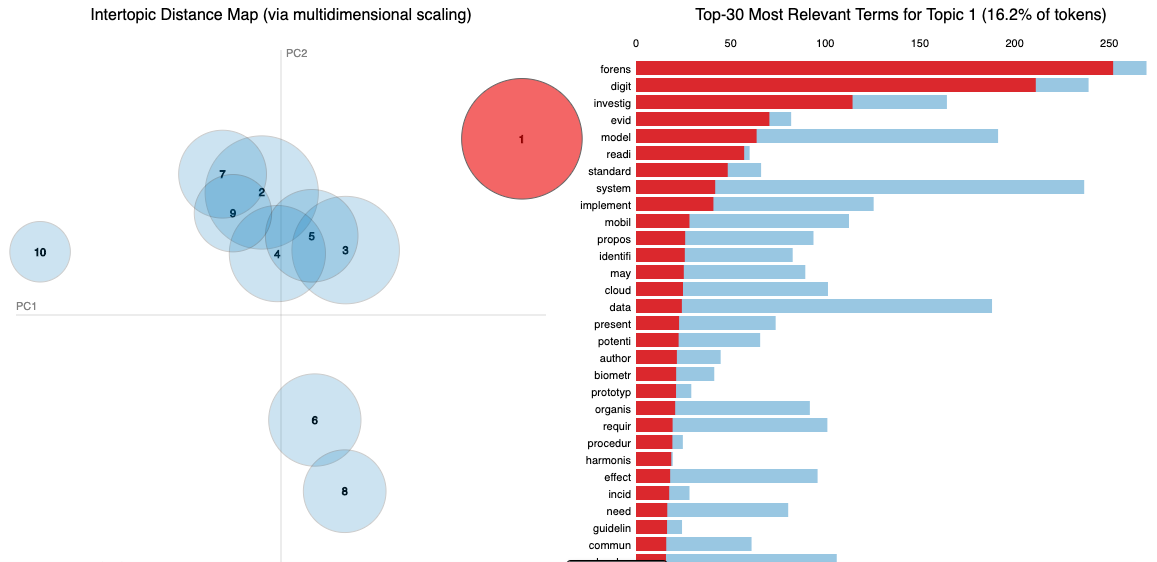
\includegraphics[width=\textwidth]{./figures/LDAVIS.png}
\caption{Visualization package for LDA}
\label{fig:LDAVIS}
\end{figure}
Based on the coherence score and supported by the observations made in pyLDAvis the researcher elected the LDA parameter number of topics as 20. In the next sub section, the researcher will discuss how the similarity between the documents were calculated.

\section{Similarity between documents}
One of the main goals of this study is to present similar papers to the readers. In order to do this, the data needs to be tokenized, normalized and cleaned. After the pre-processing pipeline, the tokenized data should be transformed into a vector and fed into the Latent Dirichlet Allocation topic modelling algorithm. After a few iterations and fine tuning of the parameters within the LDA algorithm, the output data can then be used to obtain deeper findings. 

The goal of obtaining in depth information rests on the Jensen-Shannon Divergence algorithm. As seen in figure \ref{lst:jensenfunction}, we were computing the Jenson-Shannon Distance (JSD) using Scipy's entropy. JSD finds the distance between an input query (LDA topic distribution of a single document) and a big matrix (the whole corpus) as seen in line 2. In line 5 it returns an array of length m where m is the number of document in the corpus. 

Later in line 5 the square root of the Jensen-Shannon Divergence is returned because the square root of Jensen-Shannon Divergence is the Jensen-Shannon Distance. The smaller the JSD, the more similar is the two topic distributions to each other, in this case, more similar two documents are to each other.
\begin{lstlisting}[language=Python, label={lst:jensenfunction}, caption=Implementation of Jensen-Shannon similarity]
def jensen_shannon(query, matrix):
    p = query[None,:].T
    q = matrix.T
    m = 0.5*(p + q)
    return np.sqrt(0.5*(entropy(p,m) + entropy(q,m)))
\end{lstlisting}
The Jensen-Shannon function in listing \ref{lst:jensenfunction} is then implemented in listing \ref{lst:jensen}, where it actually computes the JSD and returns the top k smallest distances. These Jensen-Shannon distances was then used to find the recommendations of academic papers. 

\begin{lstlisting}[language=Python, label={lst:jensen}, caption=Jensen-Shannon function]
def get_most_similar_documents(query,matrix,k=10):
    sims = jensen_shannon(query,matrix) 
    return sims.argsort()[:k]
\end{lstlisting}

\begin{table}[]
\begin{tabular}{|l|l|}
\hline
\textbf{Title of test paper} & \textbf{Tokenized paper} \\ \hline
\begin{tabular}[c]{@{}l@{}}Testing the Harmonised Digital Forensic\\ Investigation Process Model using an \\ Android Mobile Phone\end{tabular} & \begin{tabular}[c]{@{}l@{}}{[}'test', 'harmonis', 'digit', \\ 'forens', 'investig', 'model',\\  'android', 'mobil', 'phone'{]}\end{tabular} \\ \hline
\end{tabular}
\caption{Test paper and tokenized output}
\label{tab:testdigital}
\end{table}

As mentioned in Chapter \ref{chap: Chapter 3}, the dataset was split into a training set and testing set. The testing set comprised of only one document. The document was kept aside while training the model. The test document was selected at random using a simple Python random function. The title of the test paper can be seen in table \ref{tab:testdigital}, along side the tokenized words from that one document corpus. Interpreting the tokenized data, a fairly good guess can be made of the content of the paper. The researcher translated the tokenized data as testing a model in the digital forensic field, looking at mobile phones, Android more specifically. 

\begin{table}[]
\begin{tabular}{|l|c|}
\hline
\textbf{Title of papers} & \textbf{Scores} \\ \hline
The Design of a Wireless Forensic Readiness Model (WFRM) & 0.426 \\ \hline
\begin{tabular}[c]{@{}l@{}}Mobile Forensics using the Harmonised Digital Forensic \\ Investigation Process\end{tabular} & 0.452 \\ \hline
\begin{tabular}[c]{@{}l@{}}Enhancing Digital Business Ecosystem Trust and Reputation with\\  Centrality Measures\end{tabular} & 0.498 \\ \hline
\begin{tabular}[c]{@{}l@{}}Mobile cyber-bullying: A proposal for a pre-emptive approach to risk\\  mitigation by employing digital forensic readiness\end{tabular} & 0.497 \\ \hline
Remote Fingerprinting and Multisensor Data Fusion & 0.508 \\ \hline
\begin{tabular}[c]{@{}l@{}}Real-time Distributed Malicious Traffic Monitoring for\\  Honeypots and Network Telescopes.\end{tabular} & 0.509 \\ \hline
Harmonised Digital Forensic Investigation Process Model & 0.549 \\ \hline
Digital Forensic Readiness in the Cloud & 0.579 \\ \hline
\begin{tabular}[c]{@{}l@{}}Towards a Digital Forensic Readiness Framework for \\ Public Key Infrastructure Systems\end{tabular} & 0.592 \\ \hline
Bimodal Biometrics for Financial Infrastructure Security & 0.603 \\ \hline
\end{tabular}
\caption{Similarity scores of the most similar academic papers}
\label{tab:digital}
\end{table}

Looking at the JSD output of the two topic distributions, whole corpus and the one document, a recommendation can be made. In listing \ref{tab:digital} we can see that the scores are sorted in ascending order, ranging from 0,426 to 0,603. Smaller the score the more similar that specific document is to the test document. However, no hard-coded threshold would have made a difference in identifying the top most similar documents. These most similar documents were in fact closely similar to the test document. 

\section{Conclusion}
This chapter discussed the prototype development. It outlined the importance of having a good pre-processing pipeline in place. Feeding the data that was extracted from PDF's into a JSON format file and stored on Github for easy access ability. After the data was tokenized and pre-processed, it was transformed into a vector so the LDA algorithm could use the data. Through the iterations of fine tuning the parameters of the LDA model the number of topics were chosen (20 topics) and fed into the Jensen-Shannon Divergence similarity model and the papers were all ranked based on similarity scores. Smaller similarity scores indicates that, that particular paper is very similar to the test paper.
The next chapter discusses the lessons learned while developing the prototype.
\chapter{Lessons learned}
\label{chap: Chapter 7}

The previous chapter covered the steps taken to build a prototype of the model presented in Chapter \ref{chap: Chapter 5}. The purpose of the prototype was to act as a driver to test various techniques. The prototype was refined based on similarity scores. 

In this chapter, the algorithms and techniques are discussed in greater detail. The chapter will start off by discussing the rationale when picking pre-processing techniques, sparking the discussion around the gensim LDA algorithm, whether the antecedent algorithms and techniques influenced the similarity measures and lastly, evaluating three topics.


\section{Pre-processing}

In this section, the aim is to discuss pre-processing techniques and the significance of choosing the correct combination. Every natural language processing project has its own set of pre-processing techniques; this study is no different. The combination of techniques were derived from literature, as discussed in Chapter \ref{chap: Chapter 3}.

At first, combining the set of techniques was simple to do. However, by the time the data was at the end of the pipeline, quality inconsistencies could be seen in Listing \ref{lst:datastopwords}. This established the challenge to clean the data to a satisfactory level.

\begin{lstlisting}[language=Python, label={lst:datastopwords}, caption=Custom list of stopwords]
'unfortunately','huge','used','myburg@gmail.com','information',
'security','aodv','A12fD','derive'
\end{lstlisting}

The removal of stopwords can be bundled into a three-part process: (1) regular expressions, (2) removing the stopwords, and lastly, (3) removing the ligature characters. Throughout the process, three lessons were learned, not only during the experimentation stage of the study, but also during the refinement phase.

During the experimentation stage of the study, the first takeaway was that being too strict with the words in the stopword list would have a negative impact on the quality of the topics. However, leaving out stopwords on purpose would render the same results.

\begin{lesson}[Goldilock's dilemma]
The identification and removal of stopwords is a very important part of the pre-processing pipeline. Removing too many domain-specific words negatively influences the quality of the topics, and ultimately influences the similarity scores.
\end{lesson}\label{L:goldilocks}

Removing too many stopwords would increase the risk of losing the context of the topics, since the approach of this study is to employ unsupervised learning methods, which makes context key.

Leaving too many stopwords in the pipeline, will make the trained model convoluted. The model will then soft cluster topics, which brings no significant value and will result in inaccurate recommendations.

The optimal number of domain-specific words which are in included in the stopword list should solely be based on experimentation.

Building on the customisation of the stopword list, a second lesson was learned. Researchers used different tools for typesetting, where ligatures occur. Modern typesetting tools use updated fonts, which do not use ligatures. The problem with it was that the pre-processing techniques could not identify the ligatures and let them passed unscathed, ending up in the dataset.

\begin{lesson}[Problematic ligature characters]
Researchers using different tools for typesetting can result in the pre-processing pipeline excluding words containing ligature characters.
\end{lesson}\label{L:ligature}

Reducing dimensionality by using pre-processing did play a major part in the time performance of the algorithms. It decreased the time it took to train the models. There were 5446 unique words in the dataset without removing stopwords. Furthermore, removing more domain-specific words lowered the unique words count to 3376. Even though the unique words were reduced, we still needed to apply LDA to the words.

\section{LDA Parameters}

As described in Chapter \ref{chap: Chapter 6}, Section \ref{ssec:LDA}, latent dirichlet allocation has five parameters and two hyperparameters, which need refinement in order to achieve quality topics. However, only four parameters and two hyperparameters will be considered as they are the only parameters which need refinement.

The quality of the topics were measured in two ways: by using topic modeling evaluation techniques and human intervention by the researcher. First, the coherence score and perplexity were calculated. It should be noted that a higher coherence score indicates quality topics and simultaneously, a low perplexity score also indicates quality topics.

Manual intervention has been used in this study to validate the recommendations made. This was done by looking at the test paper, identifying a few dimensions like:

\begin{enumerate}
    \item What is the main topic discussed in this paper?
    \item What are the secondary topics discussed in this paper?
    \item What is the argument made by the researcher in this paper?
\end{enumerate}

Once the dimensions were identified, a similar exercise was done on the training set.
The recommendations was an output of 5 most similar papers, ranked from the lowest Jensen-Shannon Divergence score (most similar), to the highest JSD score.

The researcher then looked at the 5 recommended papers and compared the above-mentioned dimensions to the test paper. In most cases some of the recommendations were similar. Once the researcher identified some recommendations to be not similar, the researcher looked at how changing the LDA parameters would affect the coherence, perplexity scores and, ultimately influence the recommendations.

Human intervention was needed to validate if good coherence and perplexity scores translated into good recommendations. The observation was that for some it was true, however, some recommendations with good coherence and perplexity scores were not good recommendations. The researcher looked at the coherence and perplexity scores for the LDA parameters of the recommendations.

As mentioned, the number of papers that are recommended is 5. This number could be increased to see when the recommended papers stopped being similar however, the study focused on getting the 5 most similar papers and see how similar they are to the test paper.

\begin{lesson}[Manual intervention]
When evaluating the quality of the topics generated by the model, even though evaluation techniques like coherence scores or perplexity indicate good topics, manual intervention is still needed to validate them.
\end{lesson}\label{L:manual}

Every LDA model first needs to establish a base model to gauge a baseline. As mentioned in Chapter \ref{chap: Chapter 6}, Section \ref{ssec:LDA}, the number of topics was chosen as 20. Since establishing a base model needs human intervention to identify and to separate good results from the rest, most of the initial parameter values were chosen based on previous literature and through experimentation \cite{baghel2010frequent}. Optimising for these parameters may not yield humanly interpretable results.

The LDA parameters needed to be constant throughout the refinement process. The only parameter that changed was the one that was closely monitored. The parameter values were:

\begin{enumerate}
    \item Number of topics - 20
    \item Chunksize - 20
    \item Passes - 20
    \item Minimum probability - 0.001
    \item Alpha - 0.1
    \item Beta - 0.9
\end{enumerate}

In the rest of the section, the lessons will be discussed that were learned regarding parameter refinements. 

\subsection{Passes}

Exploring the effect that passes have on the model showed a number of interesting observations. When the number was set to 2 passes, the model trained within two seconds. The perplexity score was -7.574; this was by far the highest score from all of the tests. In addition, the coherence score was also low with 0.3056, which is significantly lower than the rest.

Next, the passes parameter was set to 200. This yielded better results than the previous one. However, the trade-off was that the model took 1.185 minutes to train. The perplexity score did improve by 0.3 to -7.3099, and the coherence score also improved to 0.4668.

Lastly, the researcher chose the value 20. The model trained significantly faster than the previous test. It took merely 8.28 seconds to train the model, which is a 758\% increase on the previous test. Perplexity and coherence scores were -7.4 and 0.4411, respectively.

The lesson learned was that the performance gain with regard to model training speed was much better than the increase in quality of the topics. Passes parameter 2 and 200 both had trade-offs: quality and speed, as referenced in Table \ref{tab:passes}.

\begin{lesson}[Quality over quantity]
Increasing the number of passes does not automatically increase the quality of the topics.
\end{lesson}\label{L:quality}

\begin{table}[]
\centering
\begin{tabular}{|l|c|c|c|}
\hline
Number of passes & 2 & 20 & 200 \\ \hline
Time to train the model & 0.020 Min & 0.138 Min & 1.185 Min \\ \hline
Perplexity & -7.574 & -7.400 & -7.3099 \\ \hline
Coherence Score c\_v & 0.3056 & 0.4411 & 0.4668 \\ \hline
\end{tabular}
\caption{Results on the number of passes}
\label{tab:passes}
\end{table}

Through human intervention, the researcher evaluated the topics to see whether they were making sense. With the lower passes parameter set, it was observed that the topics could be read and identified. However, some topics were spotted containing words which does not fit the topic it was in.

\subsection{Chunksize}

As per the definition, chunksize refers to the number of documents to be used in each chunk. It is also one of the optional parameters in the gensim LDA library. In principle, chunksize should not have an effect on the quality of the LDA topics. However, after testing the model with various sets of chunksize parameters, the numbers shows a different story.

As seen in Table \ref{tab:chunksize}, a chunksize of 20, 125, and 253 greatly affected the time taken to train the model, the perplexity value and lastly, the coherence score.

\begin{table}[]
\centering
\begin{tabular}{|l|c|c|c|}
\hline
Chunksize & 20 & 125 & 253 \\ \hline
Time to train the model & 0.083 Min & 0.059 Min & 0.135 Min \\ \hline
Perplexity & -7.377 & -7.523 & -7.422 \\ \hline
Coherence score c\_v & 0.591 & 0.394 & 0.4674 \\ \hline
\end{tabular}
\caption{Results of adjusting the chunksize.}
\label{tab:chunksize}
\end{table}

It was anticipated that reducing the chunksize, the model would take longer to train. Looking at the time values in Table \ref{tab:chunksize}, with a size of 20 the model trained in 0.083 minutes (4.98 seconds). Furthermore, changing the chunksize parameter to roughly half of the total number of documents, 125, the model trained in 0.059 minutes (3.54 seconds). Using 125 chunksize decreases the time the model took to train by 28.91\%. In contrast to using 253 as the Chunksize, which includes all the documents in the testing set, the time it took to train the model increased to 0.132 min (7.92 seconds). Comparing the difference in time the model took between 20 and 254 chunksizes was 37.12\%.

Moving to the perplexity scores of each iteration: 20, 125, and 253, respectively, a chunksize of 20 produced a perplexity score of -7.377, which was the lowest compared to all the others. This signifies that the model using a chunksize of 20 produced better topics then the rest. However, this means that it is only slightly better than using 125 and 253 chunksizes. A perplexity score of -7.377 is an increase of 1.9\% and 0.6\% compared to using the other chunksize numbers.

The coherence score of these tests proved that using a smaller chunksize does take longer to train the model; however, it does yield better results. As seen in Table \ref{tab:chunksize}, using a chunksize of 20 outperformed the rest by a big margin. Comparing the test sets, 20 to 125, and 20 to 253, there was a decrease in coherence score by 33.33\% for the first comparison and a further decrease by 20.9\% for the second comparison.

The lessons learned when comparing these above-mentioned results lead to the following point. After each test set the researcher looked at the topics to evaluate the readability and to see whether the topics can be interpreted to something of value. However, after close inspection, no noticeable difference could be flagged.

\begin{lesson}[Chunksize has little influence]
Increasing the chunksize does not have a significant influence on the quality of the topics.
\end{lesson}\label{L:chunksize}

\subsection{Minimum-probability}

As unwanted words filter through the pre-processing pipeline into the trained model, one of the ways to combat this is to have a minimum probability value set. Table \ref{tab:minimum} shows how using no minimum probability threshold can run the risk of picking up unwanted words, which translate to topics.

\begin{table}[]
\centering
\begin{tabular}{|l|l|}
\hline
\textbf{Probability} & \textbf{Topic} \\ \hline
0.002 & softlift \\ \hline
0.001 & distanc \\ \hline
0.001 & popul \\ \hline
0.001 & residenti \\ \hline
0.001 & dcss \\ \hline
0.001 & profil \\ \hline
0.000 & wherea \\ \hline
0.000 & incom \\ \hline
0.000 & strongli \\ \hline
\end{tabular}
\caption{Using minimum probability as 0.00}
\label{tab:minimum}
\end{table}

Table \ref{tab:prob} details the results of testing different minimum probability values. Setting the various probability values did not yield any impact on the time it took to train all the models. One would expect to see the model being trained faster as the minimum probability value increased. This was, in fact, the case. Comparing the perplexity score of the three models revealed that increasing the probability value did not impact the perplexity score.

\begin{table}[]
\centering
\begin{tabular}{|c|c|c|c|}
\hline
\multicolumn{1}{|l|}{Minimum Probability} & 0.00 & 0.001 & 0.1 \\ \hline
Time to train the model & 0.081 Min & 0.078 Min & 0.077 Min \\ \hline
Perplexity & -7.381 & -7.385 & -7.381 \\ \hline
Coherence score c\_v & 0.444 & 0.536 & 0.6203 \\ \hline
\end{tabular}
\caption{Results of testing minimum probability values.}
\label{tab:prob}
\end{table}

It was highly anticipated that minimum probability would have a direct impact on the coherence score since it measures the quality of the topics. The take-away from these refinements was that, as the time and perplexity score were not affected by the parameter, the coherence score was.

The value of 0.1 produced the best coherence score; however, human intervention needed to take place. Increasing the value to 0.1 meant that infrequently used terms would be disregarded. In the context of this dissertation, the data set consists of abstracts which do not contain a large text.

In light of the results shared in Table \ref{tab:prob}, the researcher chose the minimum probability of 0.01 to be used in the main model. The lesson learned was that if the parameter minimum probability was tweaked too high, most of the words that would add context to each set of topics would be omitted. This being an unsupervised machine learning proposed model, running certain risks would be unavoidable. It was all about getting the threshold.

\begin{lesson}[Probability Dilemma]
If the minimum probability is set too high, the topic model runs the risk of not including certain topics. Smaller documents often only have a few sentences, which influences the probability of word occurring. Therefore, the minimum probability cannot be too high.
\end{lesson}\label{L:probability}

\subsection{The number of LDA topics}

In Section \ref{ssc:lekker}, the systematic process was discussed that was used in determining the number of LDA topics. In addition to that, lessons were learned throughout the process and will be discussed in this section.

The tests varied from 10 topics to 35 topics. In Listing \ref{lst:cv}, the fluctuating topic coherence scores were a quantitative indication of the most suitable number of topics. However, the process still needed human intervention to confirm that the topics were making logical sense.

Keeping in mind that the corpus (ISSA Conference papers) was rich in topics, the conference papers contained about 15 primary and secondary topics; essentially, picking 10 or 15 LDA topics to try to represent the topics from the text failed.

The first lesson that was learned in this process was that a low number of LDA topics will not represent the true topic depth of the text. In Listing \ref{lst:5topics}, only five topics were chosen and we can derive the general themes they represent. Running the model again will render different results; thus showing that lowering the number of topics will result in wasting potential LDA topics and ultimately skew our recommendation at the end of the pipeline.

It is understood that every time the model runs, there is a chance that it will provide slightly different results. However, increasing the number of LDA topics would provide a safety net that the strong topics will always prevail.

\begin{lstlisting}[language=Text, label={lst:5topics}, caption=5 Number of topics]
Topic 1 - 0.016 system + 0.016 user + 0.011 social + 0.011 privaci + 0.010 manag
Topic 2 - 0.027 south + 0.024 risk + 0.016 africa + 0.015 popi + 0.013 govern
Topic 3 - 0.063 forens + 0.054 digit + 0.042 investig + 0.020 data + 0.014 databas
Topic 4 - 0.030 network + 0.025 mobil + 0.022 attack + 0.019 detect + 0.018 applic
Topic 5 - 0.027 cloud + 0.022 servic + 0.017 comput + 0.015 pattern + 0.012 face
\end{lstlisting}

In Table \ref{tab:numtopics}, three tests were undertaken, which included time taken to train the model based on the number of topics, the perplexity values per number of topics and lastly, the coherence score of each.

It was to be expected that the time would increase as the number of topics grew in size. The time increased by 49.05\%, and then by 58.22\% starting from five topics to 20 and ending off with 50 topics.

\begin{table}[]
\centering
\begin{tabular}{|c|c|c|c|}
\hline
\multicolumn{1}{|l|}{Number of LDA topics} & 5 & 20 & 50 \\ \hline
Time to train the model & 0.053 Min & 0.079 Min & 0.125 Min \\ \hline
Perplexity & -7.341 & -7.488 & -7.611 \\ \hline
Coherence score c\_v & 0.34 & 0.35 & 0.41 \\ \hline
\end{tabular}
\caption{Results of testing different number of LDA topics.}
\label{tab:numtopics}
\end{table}

Furthermore, the lesson learned from observing the perplexity score over time in Table \ref{tab:numtopics}, was that with every step from five to 20 to 50 topics, the score gradually decreases. It is to be expected that the perplexity score will flatten out as the number of topics increase. However, as stated in a previous lesson learnt, human intervention will be needed to validate whether the topics still make semantic and logical sense.

\begin{lesson}[Flatten the curve]
The perplexity score will flatten out as the number of topics gradually increase.
\end{lesson}\label{L:perplexity}

Looking at the coherence score, which also gradually changes over time, human intervention is still needed. The coherence score increases with 2.9\% and 17.14\% with each increase of topics.

\section{Latent dirichlet allocation hyperparameters}

In this section the lessons learned regarding the two hyperparameters, alpha and beta, will be discussed. The hyperparameter beta will be also referred to as eta (gensim).

Figure \ref{fig:alphaandbeta} illustrates the interconnectivity between documents, topics and words, furthermore, showing that favouring one of these two hyperparameters will result in either of two things:

\begin{itemize}
    \item High alpha - the documents will have high number of topics contributing to them.
    \item High beta - the topics have a high number of words contributing to them.
\end{itemize}

\begin{figure}[htbp]
\centering
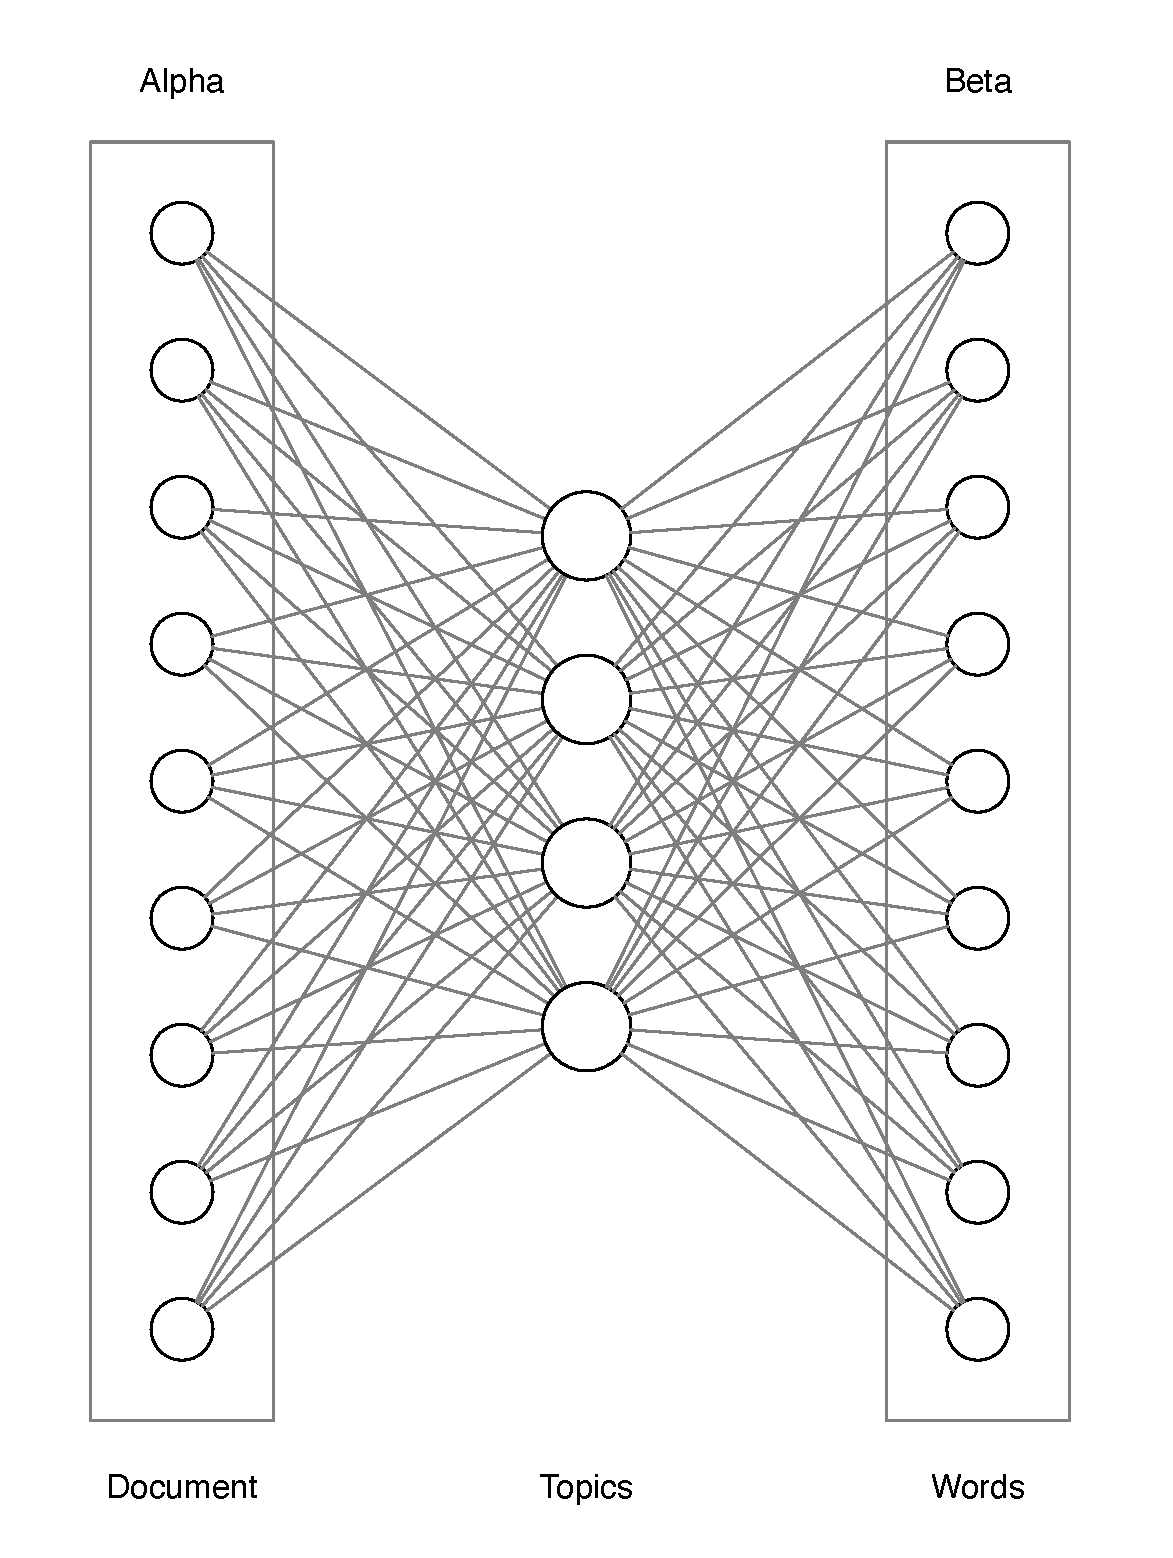
\includegraphics[width=12cm]{./figures/alpha1.eps}
\caption{Alpha and beta representation}
\label{fig:alphaandbeta}
\end{figure}

In the rest of this section, the lessons learned for both of these hyperparameters will be discussed.

\subsection{Dirichlet hyperparameter alpha}

Choosing a value of alpha or beta (eta) can be a tricky task, since these two hyperparameters have an direct impact on the topic modeling results. A high alpha means the documents contain more topics.

The researcher experimented with various alpha values. These values were 0.01, 0.1, and 0.5. It was discovered that using the above-mentioned values, the actual prototype was displaying run time divided by zero errors. The cause of the errors was linked to the alpha and beta values. The model was producing explicit zero results. 

As \citeA{wallach2009rethinking} mention, an alpha asymmetric is good, but an asymmetric beta is not. It was because of the run time errors that it was decided to set the parameters to auto. This means that the model learns an asymmetric statistical inference, or prior for short.
The hyperparameter beta will be discussed in the next sub-section.

\subsection{Dirichlet hyperparameter beta}

It was also found that experimenting with various beta (eta) values rendered the same run time errors observed with the alpha testing. The researcher also decided to set the hyperparameter to auto, which learns asymmetric prior from the data.

This approach of setting the hyperparameters to auto, as stated, was found to benefit the topics generated by the LDA model. Giving the ability to the data to learn their own prior meant that it should deliver similar results each time the model ran. Capping or limiting the hyperparameters would result in run time errors and skewed results.

As mentioned by \citeA{griffiths2004finding}, when working with scientific documents, it is best to use a larger beta (eta) value. The reason is that it could lead to the model containing a smaller number of topics and could cover more scientific concepts. This is in contrast to using a smaller beta (eta) value, which would produce more topics that would address specific concepts.

In the next section, similarities will be discussed between the probability distributions.

\section{Similarity between probability distributions}

In this section, lessons learned will be shared on the process of finding the similarities between the documents.

In Section \ref{JSD}, Jensen-Shannon Divergence (JSD) was mentioned to be the improved method used to measure similarity between two probability distributions. The researcher used the Jensen-Shannon Divergence method to calculate the distance between the two probability distributions. In recent years, research has indicated that JSD still has relevance today \cite{tong2016text,giles2019subject,he2015topic,chu2010topic}.

As there are no parameters with Jensen-Shannon Divergence, this made it easy to implement it into the prototype and ultimately, to look at the end results. Since the goal of this research was not to compare other similarity measurement methods, the researcher only considered JSD.

In the next section, evaluating the output of the similarity of the probability distributions will be discussed.

\section{Evaluation} \label{ssec:eval}

In this section the observations will be discussed between the test document and training documents. Observations will be shared to understand whether and what made the similarity list good or bad. In the next subsection a single test document with its corresponding list of similar documents will be discussed. 

The layout of the subsection will include observations on what made a topic like digital forensics and similar documents good, what LDA parameters could contribute to the change of similar documents, and how many documents matched. This structure will continue with what was considered a good match and what a bad match.

In addition to the layout of the subsections, two topics were selected to demonstrate the prototype and model. More topics were used in the experiment, however, these two topics were selected to illustrate the lessons which were learned during the study. Data related to the the other topics can be viewed in Appendix \ref{appendix: Appendix A}.

\subsection{Digital Forensics}

The title of the test document was ‘Towards a Framework for Enhancing Potential Digital Evidence Presentation’. The contents of the document covered working towards a framework to develop methodologies and specifications. The ultimate goal is to enhance the presentation and interpretation of any legal proceedings effectively.

The recommendation list of documents of the above topic consists of five documents. The list of recommendations are listed in Table \ref{tab:digitalforensics}. Observing the list, one could argue that the topic, digital forensics, was a good topic to test with.

\begin{table}[]
\centering
\resizebox{\textwidth}{!}{%
\begin{tabular}{|l|l|}
\hline
\textbf{JSD SCORE} & \textbf{TITLE} \\ \hline
0.5372 & Towards a digital forensic science \\ \hline
0.6170 & A model for secure value-added service subscriptions in cellular networks \\ \hline
0.6172 & \begin{tabular}[c]{@{}l@{}}POPI act - Opt-in and opt-out compliance from a data \\ Value chain perspective: A South African insurance industry experiment\end{tabular} \\ \hline
0.6179 & Team formation in digital forensics \\ \hline
0.6306 & The current state of digital forensic practitioners in South Africa \\ \hline
\end{tabular}%
}
\caption{Digital forensic similarity}
\label{tab:digitalforensics}
\end{table}

The researcher observed that one of the reasons that digital forensics was a good topic to test with was that there were multiple documents covering the same topic. This meant that the LDA model had more training data. Having multiple documents covering the same topic provided more words for the bag of words representation of the text.

Another observation was that since Jensen-Shannon Divergence had no real parameters to adjust, little difference could be made in the greater scheme of things. The majority of the tweaking and working must be done before getting to the Jensen-Shannon Divergence. The tweaking was done in the text pre-processing, text representation, and LDA model phases of the experiment.

\begin{lesson}[JSD no parameters]
Jensen-Shannon Divergence (JSD) does not have parameters to refine, thus putting more emphasis on the refinement of the pre-processing and topic modeling components.
\end{lesson}\label{L:JSD}

In terms of changing the LDA parameters, it was observed that increasing the chunksize of the LDA model to cover all the documents in the training set yielded good results for this specific topic. In addition, increasing the number of passes during training also yielded good results.

In the next subsection, the topic privacy, similarity list and observations will be discussed.

\subsection{Privacy}

The test document that was used had the title ‘Computer monitoring in the 21st century workplace’ which laid the foundation for a workplace privacy policy that protects employees.

The recommendation list has also provided the top five documents which it considers very similar to the document above. As viewed in Table \ref{tab:digitalforensicsBA}, the titles of the documents do not indicate any privacy topics.

\begin{table}[]
\centering
\resizebox{\textwidth}{!}{%
\begin{tabular}{|l|l|}
\hline
\textbf{JSD SCORE} & \textbf{TITLE} \\ \hline
0.5612 & A profile of the distance computing student softlifter \\ \hline
0.5820 & CDMA in signal encyption and information security \\ \hline
0.6670 & Context aware mobile application for mobile devices \\ \hline
0.6671 & Towards a framwork for a network warfare capability \\ \hline
0.6676 & Adaptable exploit detection through scalable netflow analysis \\ \hline
\end{tabular}%
}
\caption{Privacy similarity}
\label{tab:digitalforensicsBA}
\end{table}

The main observation for this subsection is that words that would be more easily identifiable in the LDA model became lost in the pre-processing and LDA pipeline.

The other observation was that once the number of topics increased, it created room for the other topics also to be included. Those topics were previously the second- or third-tier topics in the LDA model.

\begin{lesson}[More is not better]
Increasing the number of topics increases the risk that topics will be included that do not provide any significant value.
\end{lesson}\label{L:more}

As simple as it may sound, compared to digital forensics, there were not many documents which dealt with privacy and workforce topics.

\section{Summary}

In this chapter, we discussed several themes while developing the prototype. What changes were needed to be made for the prototype to perform at its maximum? The other theme was the lessons that were learned while administering the changes.

The lessons learned from each component, as indicated in Figure \ref{fig:prototype}, are summarised and shared in Table \ref{tab:lessons}. The conclusion that is drawn is that pre-processing is certainly one of the most important legs in the pipeline and needs to have most of the time dedicated to it. Each component of the pre-processing process needs to be closely considered. Removing too many words can cause documents not to any similarity to others and leaving too many words can make the LDA model too sensitive.

The experimentation, analysis, and discussion enabled the creation of the model used in Chapter \ref{chap: Chapter 6}. The model outlines the steps that were needed to achieve a recommendation list. It also opened discussions so that researchers can further the research by using additional techniques and algorithms, which will be discussed in the next chapter.

\begin{table}[htb]
\begin{tabularx}{\textwidth}{|l|X|}
\hline
\textbf{Lesson name} & \textbf{Lesson} \\ \hline
1. Goldilock's dilemma & The identification and removal of stopwords is a very important part of the pre-processing pipeline. Removing too many domain-specific words negatively influences the quality of the topics and ultimately, influences the similarity scores. \\ \hline
2. Problematic ligature characters & Researchers using different tools for typesetting can make the pre-processing pipeline exclude words containing ligature characters. \\ \hline
3. Manual intervention & When evaluating the quality of the topics generated by the model, even though evaluation techniques like coherence scores or perplexity indicate good topics, manual intervention is still needed to validate them. \\ \hline
4. Quality over quantity & Increasing the number of passes does not automatically increase the quality of the topics. \\ \hline
5. Chunksize has little influence & Increasing the chunksize does not have a significant influence on the quality of the topics. \\ \hline
6. Probability Dilemma & If the minimum probability is set too high, the topic model runs the risk of not including certain topics. Smaller documents often only have a few sentences, which influences the probability of a word occurring. Therefore, the minimum probability cannot be too high. \\ \hline
7. Flatten the curve & The perplexity score will flatten out as the number of topics gradually increase. \\ \hline
8. JSD no parameters & Jensen-Shannon Divergence (JSD) does not have parameters to refine, putting more emphasis on the refinement of the pre-processing and topic modeling components. \\ \hline
9. More is not better & Increasing the number of topics increases the risk that topics will be included that do not provide any significant value. \\ \hline
\end{tabularx}
\caption{Summary of the lessons learned}
\label{tab:lessons}
\end{table}
 

\chapter{Conclusion}
\label{chap: Chapter 8}

Based on the discussion in the previous chapter, it is clear that using various Natural Language Processing and text mining techniques outlined in chapter \ref{chap: Chapter 6} would indeed be possible.
It was apparent that adjusting the parameters of the prototype also played a major part in the quality of the topics. Later such topics directly influenced the recommendation list.

This chapter provides a summary of the study to conclude the study findings. The next section will discuss how the research objectives were reached. After the section of how the research objectives were accomplished, suggestions for future research will be made.

\section{Revisiting the research objectives}

This section facilitates a discussion on how the research objectives were met. As mentioned in chapter 1, the primary research objective was to \textbf{\textit{Develop a model to recommend related research papers.}}

Achieving the primary objective depended on meeting the secondary objectives listed in Chapter \ref{chap: Chapter 1}.

\textbf{SO 1}: \textit{To identify recommender systems techniques and how they are used.}

This secondary objective was met by surveying the literature of Recommender Systems. As this secondary objective's goal was to map and understand what techniques are used in recommender systems and how researchers utilise it. I looked at the various approaches that not only fits the use case of the study but also which is relevant. It was decided that the Content Based Filtering approach would the best to use since no assumptions are made of users activity. In addition to this, CBF does not care about user ratings, it looks at the content of the documents. It was critical to look for approaches that does not rely on user activity and user ratings. Chapter \ref{chap: Chapter 2} was dedicated to introduce the concepts of how modern Information Systems (Recommender Systems) work and how they evolved from the past to recent years. A continuation on the introduction to the fields was found in Chapter \ref{chap: Chapter 3}.

\textbf{SO 2}: \textit{To identify machine learning techniques that assist with the recommender task.}

This secondary objective was met by surveying several machine learning techniques. The goal of this objective was to identify and better understand what machine learning techniques there are, and how they tie into recommender type systems.
Machine Learning in section \ref{ssec:MLoverview}, Natural Language Processing in section \ref{secc:LDAover} and Topic Modeling in section \ref{ssec:tmodel} paved the way to understand the technology that would be used in this study.

The selection of the topic model algorithm that would be most suitable was also stemmed from literature. More specifically in section \ref{ssec:tmodel} it was discussed that Latent Dirichlet Allocation (LDA) was a very popular choice for building such topic models. Furthermore, section \ref{ssec:LDAA} explains how LDA works, by computing hidden topic structures from documents.

Before developing the conceptual model, the research methodology was discussed in Chapter \ref{chap: Chapter 4}. More specifically the research process that will be followed to conceptualise the model based on the previous chapters

Formulating the concepts into a plan of action, Chapter \ref{chap: Chapter 5} was introduced. The conceptual model was developed by looking at content covered in Chapters \ref{chap: Chapter 2} and \ref{chap: Chapter 3}. The Data Analytics lifecycle was adopted as seen in Figure \ref{fig:lifecycle} to help conceptualise the model.

Chapter \ref{chap: Chapter 6} was crucial to better understand the concepts introduced by Chapters Chapter \ref{chap: Chapter 2} and Chapter \ref{chap: Chapter 3}. The prototype served as dual purpose. The prototype highlighted parameters that has an influence on the prototype but also the overarching model. In addition to this, building a prototype using concepts in the other chapters helped the model proved that the model is feasible. Using information security research papers with security specific wording also proved the model to be applicable to domains like information security.

Throughout the prototype and model development, practical lessons were learned. Those reflections 
were shared in Chapter \ref{chap: Chapter 7}. Especially, looking at Figure \ref{fig:processing1}, we can see which lessons were learned for each phase of the conceptual model.

In the next section, we discussed the proposed model.

\section{The Proposed Model}

\begin{figure}[htbp]
\centering
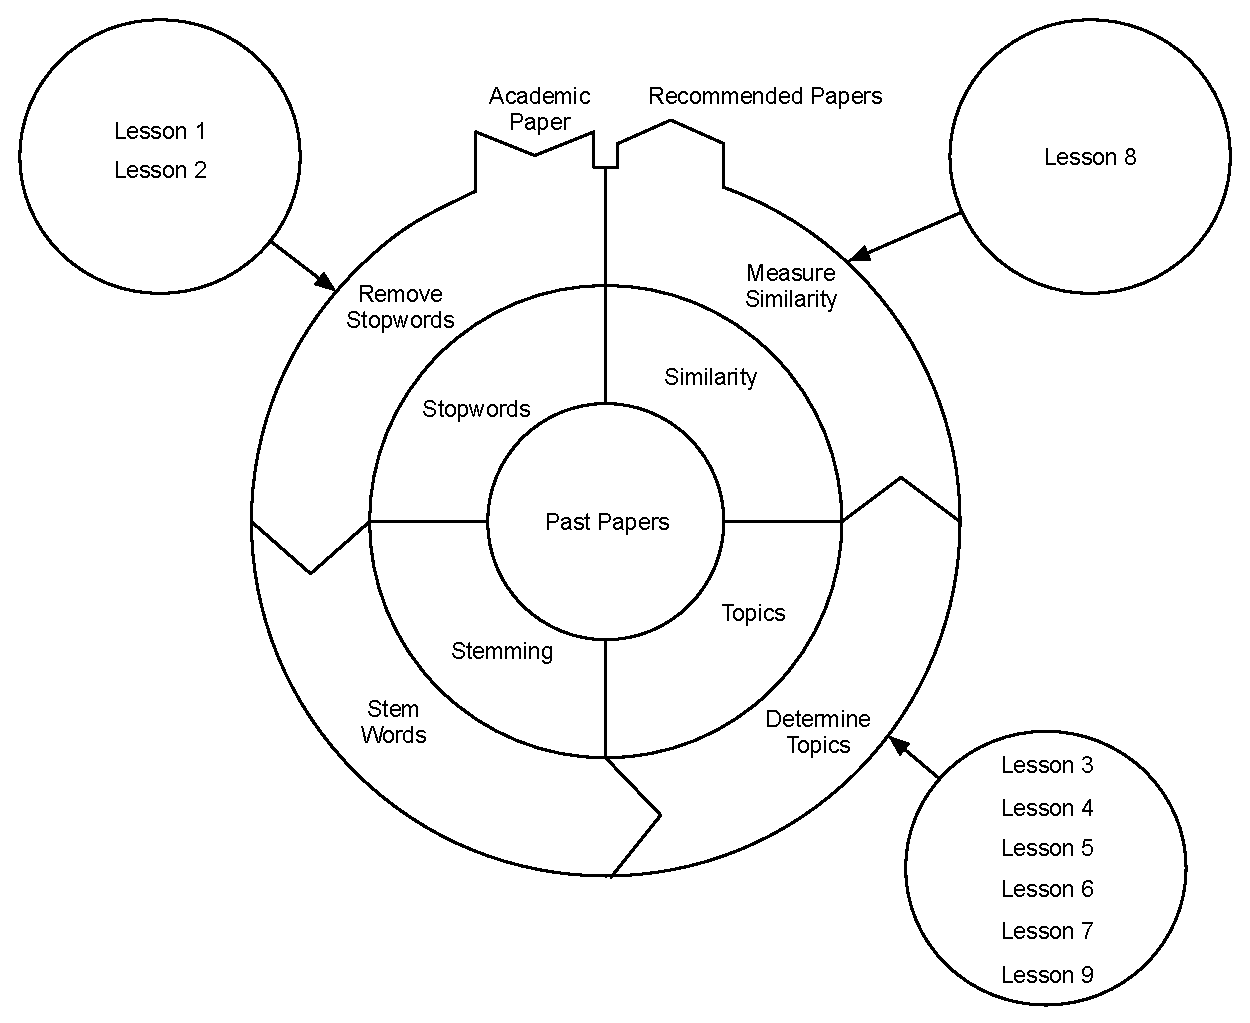
\includegraphics[width=15cm]{./figures/Lesson.eps}
\caption{Mapping lessons learned to the model}
\label{fig:processing1}
\end{figure}

This section discusses the proposed model of this study, which met the primary research objective \textbf{\textit{To develop an Recommender system which will automatically recommend similar research papers.}}

The content in chapters \ref{chap: Chapter 2} and \ref{chap: Chapter 3} set the foundation for the rest of the study. Moreover, Chapter \ref{chap: Chapter 2} focused on recommender systems, what the recommendation task entails and what the different types of recommender systems exist. 

Chapter \ref{chap: Chapter 3} explored the different machine learning technologies which are linked to recommender systems. Looking at the data that was used, the data was not labeled. As guided by literature, the suggested approach was to use unsupervised learning, to look for underlying themes. Furthermore, to help identify underlying themes document clustering which is a subset of machine learning was used in the prototype. Having two or more probability distributions, the similarity between the distributions was identified.

The suggested algorithms and processes in the previous chapters greatly influenced the research design chapter. As this study finds itself in the exploratory sphere, it was important to understand the research paradigm. Understanding the paradigm led to choosing a set of research methods and therefore, a plan of action on how to achieve the research goals.

The conceptual model was created using literature from Chapters \ref{chap: Chapter 2} and \ref{chap: Chapter 3} and guided by Chapter \ref{chap: Chapter 4}. The conceptual model, in Chapter \ref{chap: Chapter 4}, used the Data Analytics Lifecycle and adapted to the use case of this study. A prototype was developed to help the researcher understand how all these concepts fit together.

The prototype was developed with dual purpose and was documented in Chapter \ref{chap: Chapter 6}. The prototype provided the ability to observe the influence parameters has on recommendations. The experiments were conducted and documented in Chapter \ref{chap: Chapter 7}. The other purpose was to check if the model and prototype is feasible and applicable. The researcher used technologies which are still relevant today. Using these technologies and real conference data to test the prototype deems this study feasible and applicable.

Lastly, Chapter \ref{chap: Chapter 7} hosted the discussion to what practical lessons were learned during the development of the prototype, as seen in Figure \ref{fig:processing1}. 

In summary, Figure \ref{fig:processing1} represents the collection of work done in Chapters \ref{chap: Chapter 5}, \ref{chap: Chapter 6} and \ref{chap: Chapter 7}. After constructing the conceptual model in Chapter \ref{chap: Chapter 5} based on literature, chapter \ref{chap: Chapter 6} focused on validating the conceptual model. The validation was done by developing a prototype which was outlined in \ref{chap: Chapter 6}. Lastly, chapter \ref{chap: Chapter 7} included all the lessons that was learned throughout the process constructing the model and developing the prototype.

In the next section, research limitations will be discussed.

\section{Research Limitations}
This study has some limitations that must be recognized. The first limitation is that of the sample size. At the time of data collection, the information security South Africa conference only had 254 research papers to use in the dataset. Of that 254 research papers certain topics are discussed in a small number. If the topics are scarce during training, the recommendation task will be very difficult to complete. The goal was to train and test the prototype using one specific library of one conference.

The second limitation is that only one topic modeling technique (Latent Dirichlet Allocation) was used. There were several reasons behind it namely, recent research suggested that when using Content-based approaches, Latent Dirichlet Allocation would be preferred. 
Considering time constraints as this is a Masters study, we felt to go ahead with the one topic modeling technique.

The third limitation, this study only uses Jensen-Shannon Divergence to calculate the similarity between the two data spaces (Test set and training set). Similar to the second limitation, time did not allow us to venture deeper into different similarity measures.

Lastly, the forth limitation includes not having a human factor to evaluate each phase individually. The phases which are referred to is the outputs of the Topic Modeling technique and, also the end result of the similarity measurement. 

\section{Suggestions for further research}
This section is dedicated to outline further research to be done on the limitations which was raised in the previous section. Future research could possibly be conducted using a conference that has more research papers to their disposal. It will provide more data to be clustered and ultimately better the similarity measures. This relates to the first limitation.

Reflecting on the second limitation, the study could include multiple Topics Modeling algorithms and compare the outputs. Algorithms like Non Negative Matrix Factorization (NMF) \cite{Purpura2018}, Latent Semantic Analysis (LSA) \cite{Qomariyah2019}, Parallel Latent Dirichlet Allocation (PLDA) \cite{Mukherjee2019} and Pachinko Allocation Model (PAM) \cite{Koltcov2021}. 

Similarly, the third limitation, using different similarity measures could lead to different recommendations. Furthermore, mixing different Topic Models with similarity measures could yield better results.

The forth limitation which includes human intervention to evaluate each phase could sped up the model implementation, since getting feedback every step of the way.

The four limitations can also be seen as practical lessons that the researcher has learned. Along with the Table \ref{tab:lessons}, suggestions for further research and lesson learned can be seen as the same.

\section{Epilogue}
This study identified that it's time consuming for researchers to look for related research papers. This problem was addressed by developing a model to recommend related research papers. During the development of the model and prototype, it was evident that machine learning bridges the gap of spotting latent themes. However, the lessons learned Chapter \ref{chap: Chapter 7}, shows that when other researchers endeavour onto similar topics a great learning curve awaits. The researcher hopes that this study motivates other researchers to advance the natural language processing and machine learning research angle traditional topics.




%---------------------------------------------------------------------------------------------
%  The Bibliography part is fairly standard in any document
%---------------------------------------------------------------------------------------------
% plain = [1], [2] etc
% alpha = [Bot01], [BE01]
% With APA citing (apacite) you can in text use
%      \cite{XXX} to produce (SName1, SName2, & SName3, 2001) style references, or
%                            (SName1 et al., 2001) depending on position in doc; also
%      \citeA{XXX} to produce SName1, SName2, & SName3 {2001) lookalikes, or
%                              SName1, et al. (2001) depending on position in doc.
%---------------------------------------------------------------------------------------------
% Although these below looks like comments the WinEdt editor will use it to build a project tree
% and the gather interface will pop up when you reference sources (provided a proj tree has been built


    %% This line ensures that you can see the
%GATHER{library.bib}
    %% bibliography in the project tree
                                 %% and that subsequently type \cite{} will pop up
                                 %% your references - Note the UNIX style / directories!
\bibliographystyle{apacite}      %% Specifies that apa citation style should be used
\bibliography{library}
                                 %% To let BibTeX collect the references from a central place
                                 %% is a good idea.  You will be writing multiple documents
                                 %% while doing your project, but want to use one bib file
                                 %% for consistency
                                 
\appendix  % Sorts out the different page numbering, heading numbering etc.

%\part{Appendices}

%\chapter{Academic Publications}
\begin{tcolorbox}
Appendix A includes the academic papers that were written throughout the duration of the study. These papers include blah blah blah:
\begin{enumerate}
	\item 1  
	\item 2
	\item 3
\end{enumerate}
\end{tcolorbox}

\section{1}
\label{apen:1}
\begin{tcolorbox}
	\emph{Description of Paper 1}
\end{tcolorbox}

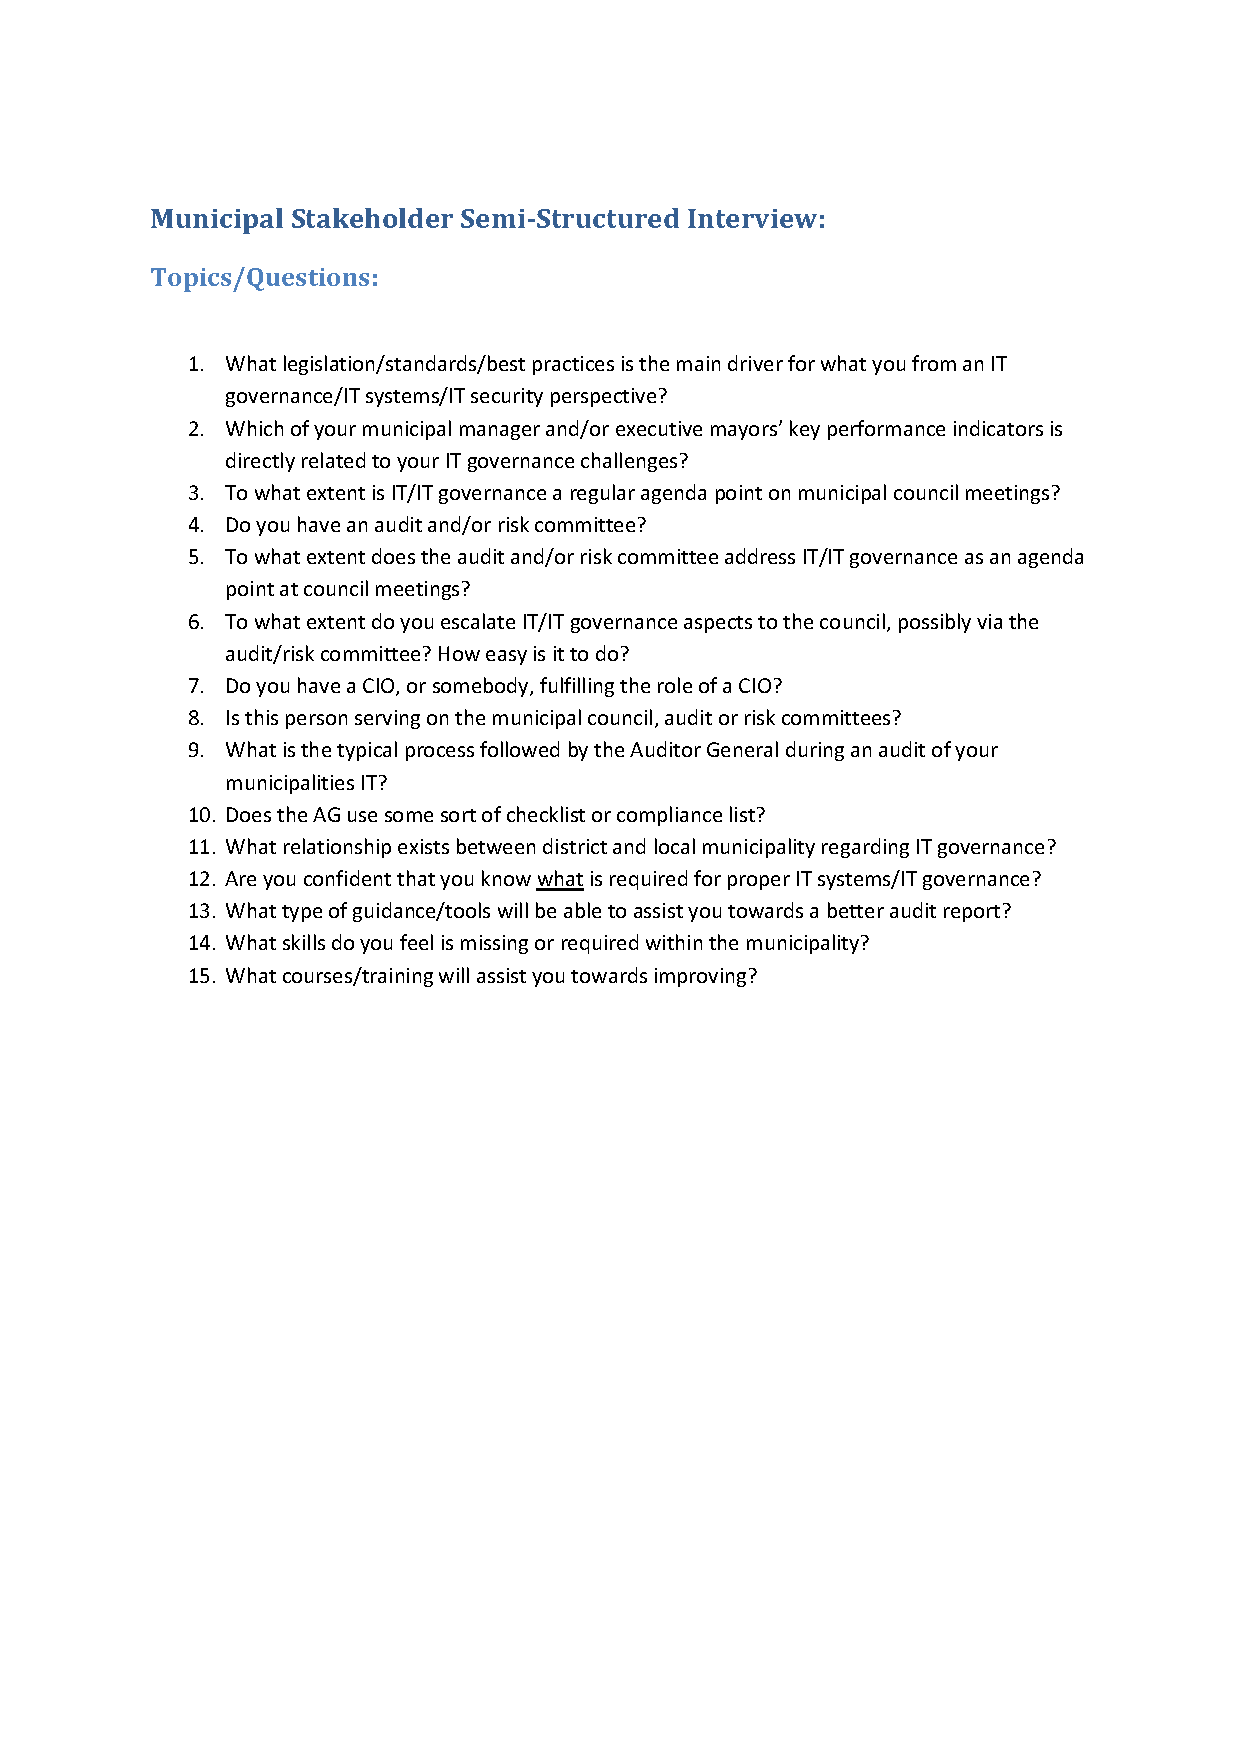
\includepdf[scale=0.9, pages=-, pagecommand={}]{./appendix/SemiStructured.pdf}

\section{2}
\label{apen:2}
\begin{tcolorbox}
	\emph{Description of Paper 2}
\end{tcolorbox}

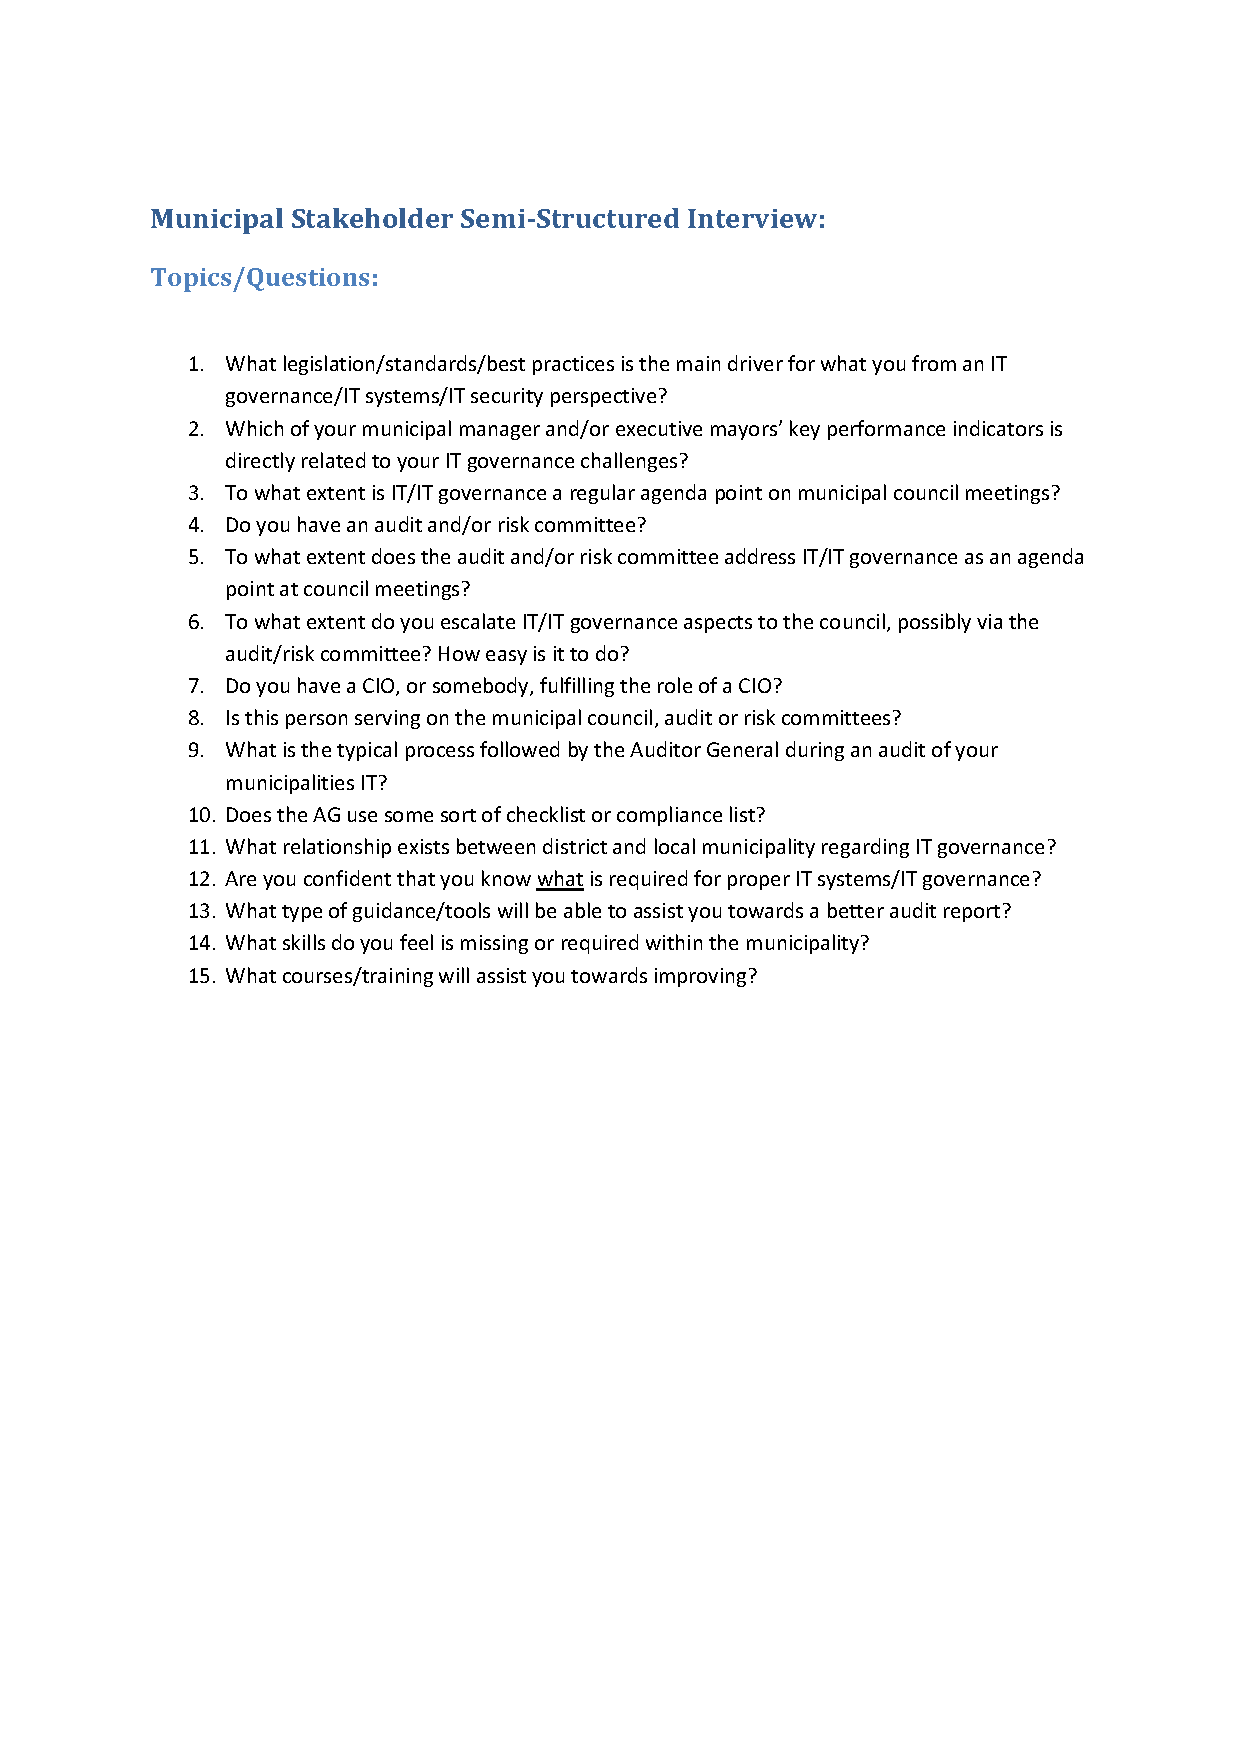
\includepdf[scale=0.9, pages=-, pagecommand={}]{./appendix/SemiStructured.pdf}

\section{3}
\label{apen:3}
\begin{tcolorbox}
	\emph{Description of Paper 3}
\end{tcolorbox}

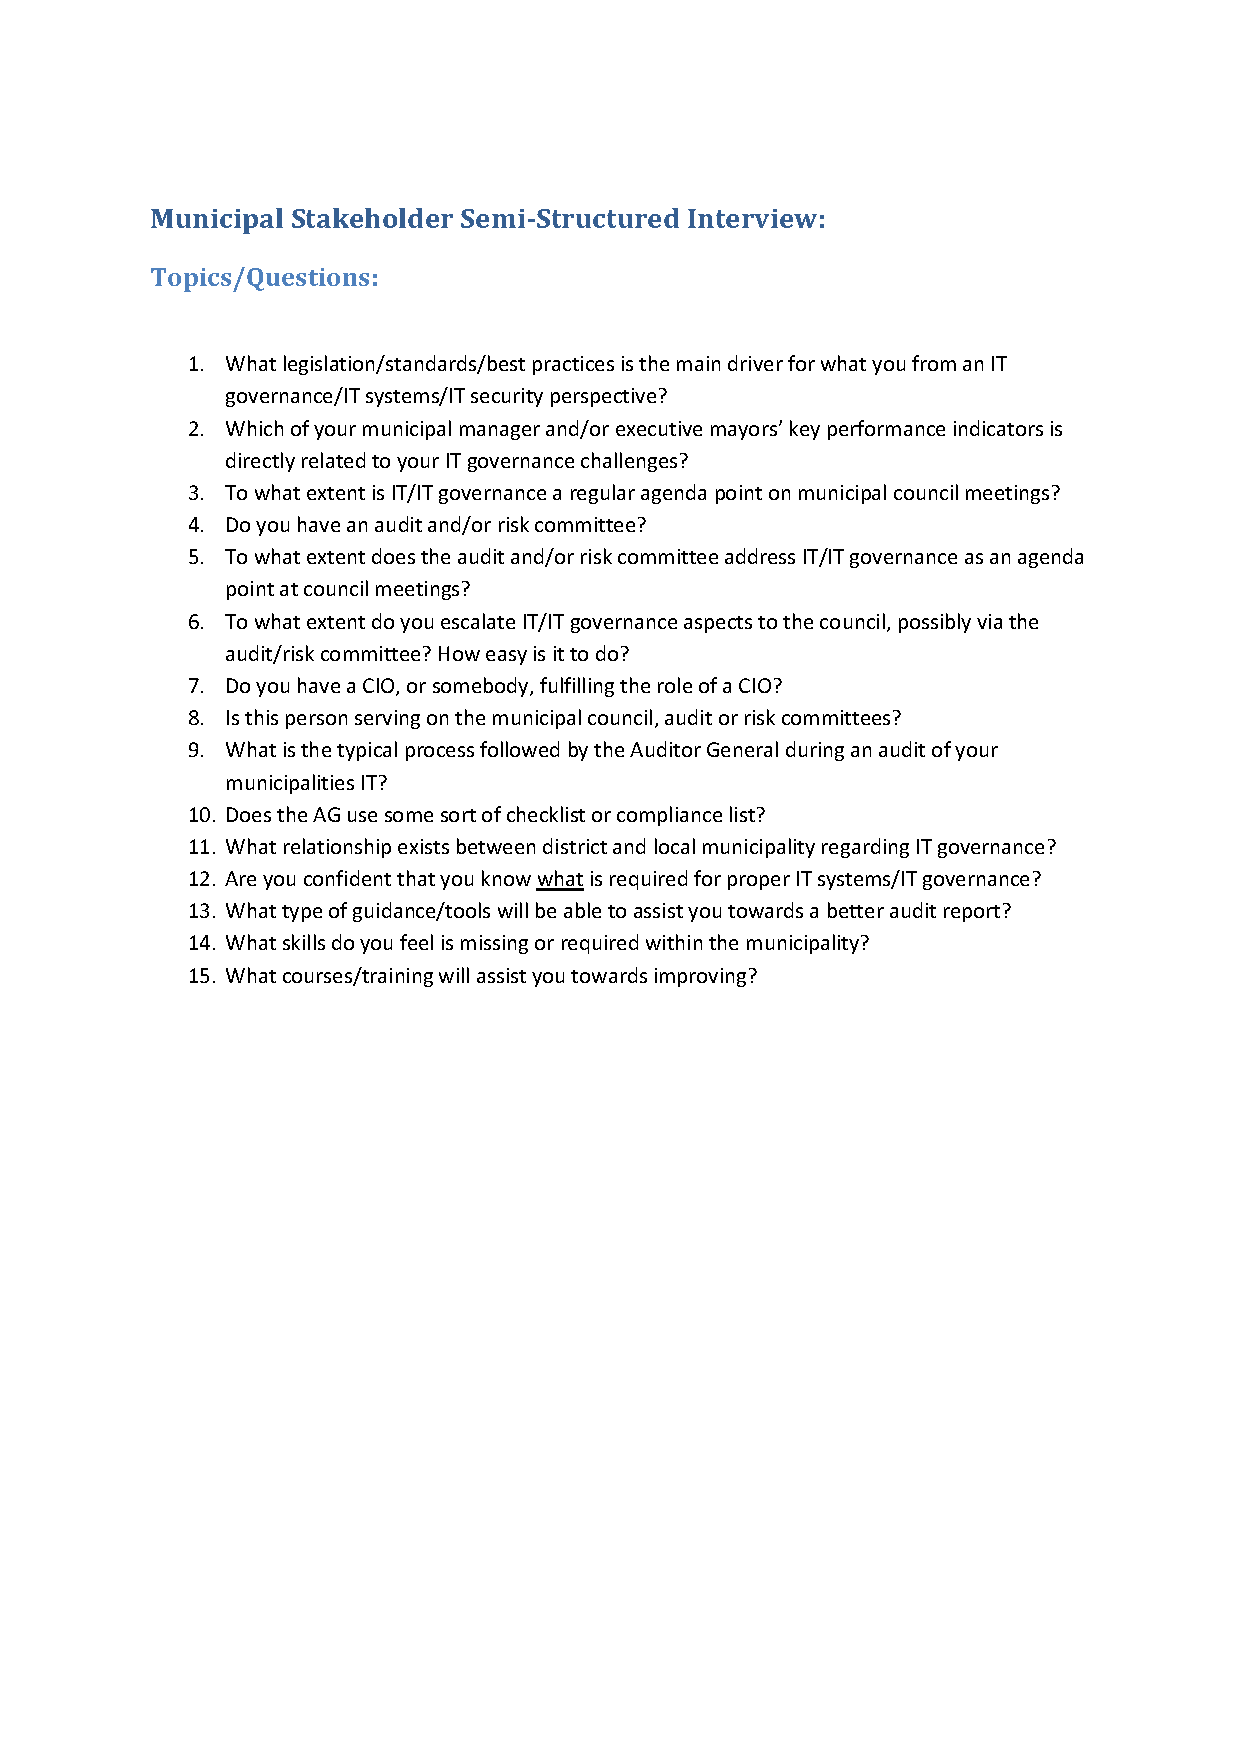
\includepdf[scale=0.9, pages=-, pagecommand={}]{./appendix/SemiStructured.pdf}
\chapter{Expansion of validation process}
\label{appendix: Appendix A}

The validation process described in Section \ref{ssec:eval}, focused on providing observations based on the demonstration of the prototype and model of two topics.
Even though Section \ref{ssec:eval} only showcased two topics, more tests were conducted which will be displayed here.

The layout of the sections will include one topic at which the top 10 recommendations were presented.

\section{Topic: Cloud Computing}
The title of the test document: ‘The Management of Security in Cloud Computing’. 

\begin{table}[htb]
\centering
\resizebox{\textwidth}{!}{%
\begin{tabular}{|l|l|}
\hline
\textbf{TITLE} & \textbf{JSD SCORE} \\ \hline
 Secure e-Government Services: Towards A Framework &  0.208068 \\ \hline
 Android Botnets on the Rise: Trends and Characteristics &  0.236715 \\ \hline
 Protection of personal information in the South-African &  0.296202 \\ \hline
 Security Foundation for a Distributed Cabin Core &  0.300801 \\ \hline
 Considering web services security policy compatibility &  0.315992 \\ \hline
 Cloud Supply Chain Resilience- A Coordination &  0.316091 \\ \hline
 Security Objectives, Controls and Metrics Development &  0.322413 \\ \hline
 Evaluating Information Security Controls Applied &  0.335019 \\ \hline
 Considering the influence of human trust in practical &   0.33537 \\ \hline
 A Software Gateway to Affordable and Effective &  0.342548 \\ \hline
\end{tabular}%
}
\caption{Security in Cloud Computing similarity}
\label{tab:cloud}
\end{table}

\section{Topic: Neural Network}

The title of the test document: ‘Filtering Spam E-Mail with Generalized Additive Neural Networks’. 

\begin{table}[htb]
\centering
\resizebox{\textwidth}{!}{%
\begin{tabular}{|l|l|}
\hline
\textbf{TITLE} & \textbf{JSD SCORE} \\ \hline
 Investigating the effect of genetic algorithms &  0.288162 \\ \hline
 Spam over Internet Telephony and how to deal with it &  0.309555 \\ \hline
 E-mail security awareness at Nelson Mandela &  0.320261 \\ \hline
 An Analysis of authentication for passive RFID &   0.32099 \\ \hline
 The use of computer vision technologies &  0.340537 \\ \hline
 The IP Protection of Electrical Databases &  0.343205 \\ \hline
 Remote Fingerprinting and Multisensor Data Fusion &  0.343431 \\ \hline
 AFA-RFID-Physical Layer Authentication for &  0.350931 \\ \hline
 Mobile Security from an Information Warfare &  0.351308 \\ \hline
 Bimodal Biometrics for Financial Infrastructure &  0.352621 \\ \hline
\end{tabular}%
}
\caption{Neural Network similarity}
\label{tab:neural}
\end{table}

\section{Topic: Smartphone Security Awareness}
The title of the test document: ‘Exploring End-User Smartphone Security Awareness within a South African context’.

\begin{table}[htb]
\centering
\resizebox{\textwidth}{!}{%
\begin{tabular}{|l|l|}
\hline
\textbf{TITLE} & \textbf{JSD SCORE} \\ \hline
 An adaptation of the awareness boundary model &  0.213688 \\ \hline
 Identity Management for e-Government Libya &  0.242323 \\ \hline
 Considering the influence of human trust &  0.247079 \\ \hline
 Factors Affecting User Experience with Security &  0.252316 \\ \hline
 Online Social Networks: Enhancing user trust &  0.272419 \\ \hline
                          Gamifying Authentication &   0.30036 \\ \hline
 Secure Cloud Computing Benefits, Risks &  0.300522 \\ \hline
 Towards achieving scalability and interoperability  &  0.300544 \\ \hline
 A formal qualitative risk management approach &  0.301527 \\ \hline
 Design of cyber security awareness game &  0.309103 \\ \hline
\end{tabular}%
}
\caption{Awareness similarity}
\label{tab:awareness}
\end{table}

\section{Topic: Bring Your Own Device}
The title of the test document: ‘A framework towards governing Bring Your Own Device in SMMEs’.

\begin{table}[htb]
\centering
\resizebox{\textwidth}{!}{%
\begin{tabular}{|l|l|}
\hline
\textbf{TITLE} & \textbf{JSD SCORE} \\ \hline
 Considering the influence of human trust &  0.207733 \\ \hline
 Protection of personal information in the South African  &  0.250983 \\ \hline
 Information Security Assurance Model (ISAM) &  0.256613 \\ \hline
 Bloom’S Taxonomy for Information Security Education &  0.257684 \\ \hline
 A survey of computer crime and security in South Africa &  0.258457 \\ \hline
 The impact of Information security awareness training &  0.259873 \\ \hline
 The Identification of Information Sources to &  0.265763 \\ \hline
 BC3I – Towards requirements specification  &  0.267988 \\ \hline
 A formal qualitative risk management approach &  0.271136 \\ \hline
 An Interactive Visual Library Model to Improve &  0.271961 \\ \hline
\end{tabular}%
}
\caption{BYOD similarity}
\label{tab:byod}
\end{table}

\section{Topic: Intrusion Detection}
The title of the test document: ‘Intrusion Detection in Bluetooth Enabled Mobile Phones’.

\begin{table}[htb]
\centering
\resizebox{\textwidth}{!}{%
\begin{tabular}{|l|l|}
\hline
\textbf{TITLE} & \textbf{JSD SCORE} \\ \hline
 A Framework of Opportunity-Reducing Techniques &  0.166268 \\ \hline
 A Conceptual Opportunity-based Framework &  0.198728 \\ \hline
                The Murky Waters of IT Governance  &  0.269619 \\ \hline
 Towards a framework for a network warfare capability &  0.282355 \\ \hline
    Combatting Phishing: A Holistic Human Approach &  0.299802 \\ \hline
 Towards a PHP Webshell Taxonomy using Deobfuscation &   0.30253 \\ \hline
 Mobile Security from an Information Warfare Perspective &  0.309996 \\ \hline
 Secure e-Government Services: Towards A Framework &  0.317646 \\ \hline
 Unsolicited Short Message Service Marketing &  0.318187 \\ \hline
 Towards a Sandbox for the Deobfuscation &   0.32363 \\ \hline
\end{tabular}%
}
\caption{Intrusion detection similarity}
\label{tab:IDS}
\end{table}
%\chapter{Questionnaires}




ncie
%\chapter{Framework for CGICT in Local Government}


\backmatter                                 

%\chapter{Expansion of validation process}
\label{appendix: Appendix A}

The validation process described in Section \ref{ssec:eval}, focused on providing observations based on the demonstration of the prototype and model of two topics.
Even though Section \ref{ssec:eval} only showcased two topics, more tests were conducted which will be displayed here.

The layout of the sections will include one topic at which the top 10 recommendations were presented.

\section{Topic: Cloud Computing}
The title of the test document: ‘The Management of Security in Cloud Computing’. 

\begin{table}[htb]
\centering
\resizebox{\textwidth}{!}{%
\begin{tabular}{|l|l|}
\hline
\textbf{TITLE} & \textbf{JSD SCORE} \\ \hline
 Secure e-Government Services: Towards A Framework &  0.208068 \\ \hline
 Android Botnets on the Rise: Trends and Characteristics &  0.236715 \\ \hline
 Protection of personal information in the South-African &  0.296202 \\ \hline
 Security Foundation for a Distributed Cabin Core &  0.300801 \\ \hline
 Considering web services security policy compatibility &  0.315992 \\ \hline
 Cloud Supply Chain Resilience- A Coordination &  0.316091 \\ \hline
 Security Objectives, Controls and Metrics Development &  0.322413 \\ \hline
 Evaluating Information Security Controls Applied &  0.335019 \\ \hline
 Considering the influence of human trust in practical &   0.33537 \\ \hline
 A Software Gateway to Affordable and Effective &  0.342548 \\ \hline
\end{tabular}%
}
\caption{Security in Cloud Computing similarity}
\label{tab:cloud}
\end{table}

\section{Topic: Neural Network}

The title of the test document: ‘Filtering Spam E-Mail with Generalized Additive Neural Networks’. 

\begin{table}[htb]
\centering
\resizebox{\textwidth}{!}{%
\begin{tabular}{|l|l|}
\hline
\textbf{TITLE} & \textbf{JSD SCORE} \\ \hline
 Investigating the effect of genetic algorithms &  0.288162 \\ \hline
 Spam over Internet Telephony and how to deal with it &  0.309555 \\ \hline
 E-mail security awareness at Nelson Mandela &  0.320261 \\ \hline
 An Analysis of authentication for passive RFID &   0.32099 \\ \hline
 The use of computer vision technologies &  0.340537 \\ \hline
 The IP Protection of Electrical Databases &  0.343205 \\ \hline
 Remote Fingerprinting and Multisensor Data Fusion &  0.343431 \\ \hline
 AFA-RFID-Physical Layer Authentication for &  0.350931 \\ \hline
 Mobile Security from an Information Warfare &  0.351308 \\ \hline
 Bimodal Biometrics for Financial Infrastructure &  0.352621 \\ \hline
\end{tabular}%
}
\caption{Neural Network similarity}
\label{tab:neural}
\end{table}

\section{Topic: Smartphone Security Awareness}
The title of the test document: ‘Exploring End-User Smartphone Security Awareness within a South African context’.

\begin{table}[htb]
\centering
\resizebox{\textwidth}{!}{%
\begin{tabular}{|l|l|}
\hline
\textbf{TITLE} & \textbf{JSD SCORE} \\ \hline
 An adaptation of the awareness boundary model &  0.213688 \\ \hline
 Identity Management for e-Government Libya &  0.242323 \\ \hline
 Considering the influence of human trust &  0.247079 \\ \hline
 Factors Affecting User Experience with Security &  0.252316 \\ \hline
 Online Social Networks: Enhancing user trust &  0.272419 \\ \hline
                          Gamifying Authentication &   0.30036 \\ \hline
 Secure Cloud Computing Benefits, Risks &  0.300522 \\ \hline
 Towards achieving scalability and interoperability  &  0.300544 \\ \hline
 A formal qualitative risk management approach &  0.301527 \\ \hline
 Design of cyber security awareness game &  0.309103 \\ \hline
\end{tabular}%
}
\caption{Awareness similarity}
\label{tab:awareness}
\end{table}

\section{Topic: Bring Your Own Device}
The title of the test document: ‘A framework towards governing Bring Your Own Device in SMMEs’.

\begin{table}[htb]
\centering
\resizebox{\textwidth}{!}{%
\begin{tabular}{|l|l|}
\hline
\textbf{TITLE} & \textbf{JSD SCORE} \\ \hline
 Considering the influence of human trust &  0.207733 \\ \hline
 Protection of personal information in the South African  &  0.250983 \\ \hline
 Information Security Assurance Model (ISAM) &  0.256613 \\ \hline
 Bloom’S Taxonomy for Information Security Education &  0.257684 \\ \hline
 A survey of computer crime and security in South Africa &  0.258457 \\ \hline
 The impact of Information security awareness training &  0.259873 \\ \hline
 The Identification of Information Sources to &  0.265763 \\ \hline
 BC3I – Towards requirements specification  &  0.267988 \\ \hline
 A formal qualitative risk management approach &  0.271136 \\ \hline
 An Interactive Visual Library Model to Improve &  0.271961 \\ \hline
\end{tabular}%
}
\caption{BYOD similarity}
\label{tab:byod}
\end{table}

\section{Topic: Intrusion Detection}
The title of the test document: ‘Intrusion Detection in Bluetooth Enabled Mobile Phones’.

\begin{table}[htb]
\centering
\resizebox{\textwidth}{!}{%
\begin{tabular}{|l|l|}
\hline
\textbf{TITLE} & \textbf{JSD SCORE} \\ \hline
 A Framework of Opportunity-Reducing Techniques &  0.166268 \\ \hline
 A Conceptual Opportunity-based Framework &  0.198728 \\ \hline
                The Murky Waters of IT Governance  &  0.269619 \\ \hline
 Towards a framework for a network warfare capability &  0.282355 \\ \hline
    Combatting Phishing: A Holistic Human Approach &  0.299802 \\ \hline
 Towards a PHP Webshell Taxonomy using Deobfuscation &   0.30253 \\ \hline
 Mobile Security from an Information Warfare Perspective &  0.309996 \\ \hline
 Secure e-Government Services: Towards A Framework &  0.317646 \\ \hline
 Unsolicited Short Message Service Marketing &  0.318187 \\ \hline
 Towards a Sandbox for the Deobfuscation &   0.32363 \\ \hline
\end{tabular}%
}
\caption{Intrusion detection similarity}
\label{tab:IDS}
\end{table}
%\chapter{Questionnaires}




ncie
\end{document}

% ----------------------------------------------------------------
